%%%%%%%%%%%%%%%%%%%%%%%%%%%%%%%%%%%%%%%%%%%%%%%%%%%%%%%%%%%%%%%%%%%%%%%%%%%%%%%
% Technical Notebook — Honda CALPHAD Cu Removal Project
% A comprehensive synthesis of methods, findings, and insights
% Anthony DiMascio — MSE 4381 Capstone, Spring 2026
%%%%%%%%%%%%%%%%%%%%%%%%%%%%%%%%%%%%%%%%%%%%%%%%%%%%%%%%%%%%%%%%%%%%%%%%%%%%%%%

\documentclass[11pt]{article}

% Packages
\usepackage[utf8]{inputenc}
\usepackage[T1]{fontenc}
\usepackage{lmodern}
\usepackage{geometry}
\usepackage{graphicx}
\usepackage{caption}
\usepackage{amsmath, amssymb}
\usepackage[hidelinks]{hyperref}
\usepackage{float}
\usepackage{enumitem}
\usepackage{fancyhdr}
\usepackage[table]{xcolor}
\usepackage{setspace}
\usepackage[compact]{titlesec}
\usepackage{microtype}
\tolerance=1000
\emergencystretch=2em
\usepackage{booktabs}
\usepackage{array}
\usepackage{tabularx}
\usepackage{colortbl}
\usepackage{multicol}
\usepackage{siunitx}
\usepackage{listings}
\usepackage{url}

% OSU colors
\definecolor{scarlett}{RGB}{187,0,0}
\definecolor{darkgray}{RGB}{77,77,77}
\definecolor{headercolor}{HTML}{595959}
\definecolor{altrow}{HTML}{E0E0E0}
\definecolor{codeblue}{HTML}{0077BB}
\definecolor{codeorange}{HTML}{EE7733}
\definecolor{codegray}{HTML}{F5F5F5}

% Code listing style
\lstset{
    basicstyle=\ttfamily\small,
    backgroundcolor=\color{codegray},
    frame=single,
    framerule=0pt,
    breaklines=true,
    keywordstyle=\color{codeblue},
    commentstyle=\color{darkgray},
    stringstyle=\color{codeorange},
    showstringspaces=false,
    tabsize=4,
    language=Python
}

% Page geometry
\geometry{letterpaper, margin=0.85in}

% Header/footer
\setlength{\headheight}{28pt}
\setlength{\headsep}{15pt}
\renewcommand{\headrulewidth}{0pt}

\pagestyle{fancy}
\fancyhf{}
\fancyhead[L]{\raisebox{-0.3cm}{\includegraphics[height=0.75cm]{../../assignments/OSU Logo.jpg}}}
\fancyhead[R]{%
  \begin{minipage}[c]{3.8in}
    \raggedleft
    {\footnotesize \textbf{\textcolor{darkgray}{COLLEGE OF ENGINEERING}}}\\
    {\footnotesize \textbf{\textcolor{scarlett}{DEPT.\ OF MATERIALS SCIENCE \& ENGINEERING}}}
  \end{minipage}%
}
\fancyfoot[L]{\small A.\ DiMascio}
\fancyfoot[C]{\small Technical Notebook --- Cu Removal}
\fancyfoot[R]{\small \thepage}

% Section formatting
\titleformat{\section}{\Large\bfseries}{\thesection}{1em}{\MakeUppercase}
\titleformat{\subsection}{\large\bfseries}{\thesubsection}{1em}{}
\titleformat{\subsubsection}{\normalsize\bfseries}{\thesubsubsection}{1em}{}
\titlespacing*{\section}{0pt}{2ex plus 1ex minus .2ex}{1.5ex plus .2ex}
\titlespacing*{\subsection}{0pt}{1.5ex plus 1ex minus .2ex}{1ex plus .2ex}

% Hyperlink colors
\hypersetup{
    colorlinks=true,
    linkcolor=scarlett,
    urlcolor=codeblue,
    citecolor=scarlett
}

% Graphics path
\graphicspath{{../figures/}}

% Custom environment for key insights
\usepackage{tcolorbox}
\newtcolorbox{insight}[1][]{
    colback=codegray,
    colframe=darkgray,
    fonttitle=\bfseries,
    title={#1},
    arc=2pt,
    left=8pt,
    right=8pt
}

\begin{document}

%%%%%%%%%%%%%%%%%%%%%%%%%%%%%%%%%%%%%%%%%%%%%%%%%%%%%%%%%%%%%%%%%%%%%%%%%%%%%%%
% TITLE PAGE
%%%%%%%%%%%%%%%%%%%%%%%%%%%%%%%%%%%%%%%%%%%%%%%%%%%%%%%%%%%%%%%%%%%%%%%%%%%%%%%
\thispagestyle{fancy}
\vspace*{\fill}

\begin{center}
{\LARGE\bfseries Technical Notebook\\[0.3em]
\large CALPHAD Modeling of Copper Removal\\from Recycled Steel via Oxide Slag\par}
\end{center}

\vspace{0.8in}

\begin{center}
{\large
Anthony DiMascio, Tim Kalmar, Aishwarya Muralidhar, Mohammed Oumer\\[1em]
MSE 4381 -- Design \& Professional Practice I\\
Advisor: Prof.\ Alan Luo | Post-Doc: Dr.\ Jianyue Zhang\\
Industry Partner: Honda R\&D Americas (Dr.\ Jim Hu)\\[0.5em]
Spring 2026\par}
\end{center}

\vspace{0.8in}

\begin{center}
\textit{Personal synthesis of methods, findings, and technical insights\\
from the Honda CALPHAD copper removal project.\\[0.5em]
Living document, updated as new results come in.}
\end{center}

\vspace*{\fill}
\newpage

%%%%%%%%%%%%%%%%%%%%%%%%%%%%%%%%%%%%%%%%%%%%%%%%%%%%%%%%%%%%%%%%%%%%%%%%%%%%%%%
% TABLE OF CONTENTS
%%%%%%%%%%%%%%%%%%%%%%%%%%%%%%%%%%%%%%%%%%%%%%%%%%%%%%%%%%%%%%%%%%%%%%%%%%%%%%%
\tableofcontents
\newpage

%%%%%%%%%%%%%%%%%%%%%%%%%%%%%%%%%%%%%%%%%%%%%%%%%%%%%%%%%%%%%%%%%%%%%%%%%%%%%%%
% 1. THE PROBLEM
%%%%%%%%%%%%%%%%%%%%%%%%%%%%%%%%%%%%%%%%%%%%%%%%%%%%%%%%%%%%%%%%%%%%%%%%%%%%%%%
\section{The Copper Problem in Steel Recycling}

\subsection{Why This Matters}

Recycled steel picks up copper from wiring, motors, and electronics in automotive scrap. Typical Cu levels run 0.25--0.3 wt\% and keep rising as vehicles get more electronic. The problem starts above about 0.1 wt\%: Cu segregates to grain boundaries during hot working and causes \textbf{``hot shortness''}, surface cracking that ruins the steel for body panels~\cite{Daehn2019}.

Nobody has a good industrial-scale fix. The standard workaround is diluting with virgin iron or DRI, which is expensive and defeats the purpose of recycling~\cite{Daehn2019}. Honda uses a lot of sheet steel, so they have a direct stake in solving this.

\subsection{Our Approach: CALPHAD Screening}

CALPHAD (Calculation of Phase Diagrams) uses thermodynamic databases to predict which phases are stable at a given temperature and composition~\cite{Lukas2007}. Our strategy:

\begin{enumerate}[leftmargin=*]
    \item Identify oxide materials that might \textit{capture} Cu from molten steel
    \item Compute the Gibbs free energy of Cu-capture reactions ($\Delta G < 0$ = favorable)
    \item Rank candidates by thermodynamic driving force
    \item Validate top candidates experimentally in Fontana Lab
\end{enumerate}

The key tool is TC-Python~\cite{Andersson2002, Sundman1985}, the Python API for Thermo-Calc, using the TCOX14 oxide database~\cite{TCOX14} and TCFE13 steel database.

\subsection{Project History}

This is \textbf{Year 3} of Honda's decopperization project at OSU:
\begin{itemize}[leftmargin=*]
    \item \textbf{Year 1} (Ken Kushner): Initial scoping
    \item \textbf{Year 2} (Andrew's group): Experimental tests with Al$_2$O$_3$. Some Cu reduction was observed, but Na$_2$S salt flux was more effective (95\% removal per Dr.\ Zhang, Feb 12 meeting). Na$_2$S produces toxic H$_2$S gas, motivating the oxide approach.
    \item \textbf{Year 3} (our team): Systematic CALPHAD screening of oxide candidates
\end{itemize}


%%%%%%%%%%%%%%%%%%%%%%%%%%%%%%%%%%%%%%%%%%%%%%%%%%%%%%%%%%%%%%%%%%%%%%%%%%%%%%%
% 2. THERMODYNAMIC FRAMEWORK
%%%%%%%%%%%%%%%%%%%%%%%%%%%%%%%%%%%%%%%%%%%%%%%%%%%%%%%%%%%%%%%%%%%%%%%%%%%%%%%
\section{Thermodynamic Framework}

\subsection{How CALPHAD Works}

CALPHAD models the Gibbs energy of every phase as a function of temperature and composition~\cite{Lukas2007, Hillert2007}. For a phase $\phi$:
\begin{equation}
    G_m^\phi(T, \mathbf{x}) = \sum_i x_i \,{}^0G_i^\phi(T) + RT \sum_i x_i \ln x_i + G^{\text{xs}}(T, \mathbf{x})
    \label{eq:calphad}
\end{equation}
Three terms: (1) reference energy from pure components, (2) ideal mixing entropy (the $RT\ln x$ term you see in every thermo textbook~\cite{Gaskell2024}), and (3) excess Gibbs energy for non-ideal interactions. The third term is where all the real work goes; it gets fitted to experimental data and DFT calculations~\cite{Lukas2007}.

At equilibrium, the system minimizes total $G$ by distributing components across phases. TC-Python~\cite{Andersson2002} does this numerically for systems with dozens of phases.

\subsection{Key Quantity: GM (Gibbs Energy per Mole of Atoms)}

TC-Python returns \texttt{GM}, the Gibbs energy per mole of \textit{atoms}, not per mole of formula units~\cite{Andersson2002}. This tripped us up early:

\begin{insight}[GM Normalization]
For a compound with $N$ atoms per formula unit (e.g., CuFe$_2$O$_4$ has $N = 7$):
\[
    G_{\text{per formula}} = N \times \texttt{GM}
\]
Getting this wrong gives energies off by factors of 5--7$\times$. We caught this bug early.
\end{insight}

Similarly, the O$_2$ reference requires:
\[
    G_{\text{O}_2} = 2 \times \texttt{GM}(\text{pure O at same }T)
\]
because \texttt{GM} is per O atom.

\subsection{Mole Fraction Conventions}

In TC-Python, you set $N-1$ mole fraction conditions for an $N$-component system. The last element fills the remainder. For a ternary Cu-Fe-O system modeling CuFe$_2$O$_4$ ($x_{\text{Cu}} = 1/7$, $x_{\text{Fe}} = 2/7$, $x_{\text{O}} = 4/7$):

\begin{lstlisting}
calc.set_condition("X(CU)", 1.0/7.0)
calc.set_condition("X(FE)", 2.0/7.0)
# O fills remainder: X(O) = 4/7
\end{lstlisting}


%%%%%%%%%%%%%%%%%%%%%%%%%%%%%%%%%%%%%%%%%%%%%%%%%%%%%%%%%%%%%%%%%%%%%%%%%%%%%%%
% 3. BINARY SCREENING: THE ELLINGHAM APPROACH
%%%%%%%%%%%%%%%%%%%%%%%%%%%%%%%%%%%%%%%%%%%%%%%%%%%%%%%%%%%%%%%%%%%%%%%%%%%%%%%
\section{Phase 1: Binary Screening (Ellingham Diagram)}

\subsection{The Question}

Can metallic Cu directly reduce a ceramic oxide? For example:
\[
    \text{Cu} + \text{MgO} \to \text{Cu}_2\text{O} + \text{Mg} \quad \text{(does this happen?)}
\]

You answer this by comparing standard Gibbs energies of oxide formation on an Ellingham diagram~\cite{Gaskell2024, Brown2026CALPHAD}. If Cu$_2$O is \textit{less stable} than the target oxide, Cu cannot reduce it.

\subsection{Results}

Cu$_2$O is the \textbf{least stable oxide} in our study, with a formation energy approximately \SI{800}{\kilo\joule\per\mole}\,O$_2$ less negative than Al$_2$O$_3$, MgO, or SiO$_2$. This means:

\begin{insight}[Binary Screening Conclusion]
Cu \textbf{cannot reduce any useful ceramic oxide}. All $\Delta G_{\text{rxn}} > 0$ for the binary exchange reaction. This rules out the simplest Cu removal mechanism.
\end{insight}

We extracted formation energies for 18 oxides (11 from TCOX14~\cite{TCOX14}, 2 from SSUB3~\cite{SSUB3}, 7 ``moonshot'' literature values) over 500--2000 K in 50 K steps. Every one confirms: Cu cannot reduce any of them at steelmaking temperatures.

\begin{figure}[H]
    \centering
    
\includegraphics[width=0.85\textwidth]{ellingham_diagram_tcox14.png}
    \caption{Ellingham diagram of oxide formation energies from TCOX14. Cu$_2$O (red) sits far above all candidate oxides, confirming Cu cannot reduce any of them. Script: \texttt{simulations/notebooks/ellingham\_diagram.py}.}
    \label{fig:ellingham}
\end{figure}

\subsection{Dr.\ Zhang's Pivot}

At our Feb 12 meeting, Dr.\ Zhang explained that the binary result was \textit{expected}. The real mechanism is not oxide reduction but \textbf{ternary compound formation}:
\begin{quote}
``We want to use the oxide to capture the copper. Last time, [Al$_2$O$_3$] worked because of the spinel reaction.''
\end{quote}

The reaction is not Cu $+$ Al$_2$O$_3 \to$ products, but rather:
\[
    \text{Cu} + \text{Al}_2\text{O}_3 + \tfrac{1}{2}\text{O}_2 \to \text{CuAl}_2\text{O}_4 \quad (\text{spinel})
\]
That is a completely different thermodynamic question.


%%%%%%%%%%%%%%%%%%%%%%%%%%%%%%%%%%%%%%%%%%%%%%%%%%%%%%%%%%%%%%%%%%%%%%%%%%%%%%%
% 4. TERNARY REACTION MODELING
%%%%%%%%%%%%%%%%%%%%%%%%%%%%%%%%%%%%%%%%%%%%%%%%%%%%%%%%%%%%%%%%%%%%%%%%%%%%%%%
\section{Phase 2: Ternary Reaction Modeling}

\subsection{The Ternary Reaction}

For each candidate oxide MO$_x$, we compute:
\begin{equation}
    n_{\text{Cu}} \cdot \text{Cu} + a \cdot \text{MO}_x + \tfrac{b}{2}\,\text{O}_2 \to \text{Cu}_{n}\text{M}_c\text{O}_d
    \label{eq:ternary}
\end{equation}
where the stoichiometry comes from the known ternary compound. The standard free energy of reaction~\cite{Gaskell2024}:
\begin{equation}
    \Delta G_{\text{rxn}} = G_{\text{product}} - \left[ n_{\text{Cu}} \cdot G_{\text{Cu}} + a \cdot G_{\text{MO}_x} + \tfrac{b}{2} \cdot G_{\text{O}_2} \right]
    \label{eq:dG_ternary}
\end{equation}

Each $G$ term is computed by TC-Python as a single-phase equilibrium at the compound's stoichiometric composition. \texttt{GM} $\times$ (atoms per formula unit) gives per-formula energies.

\subsection{Results: All 16 Reactions Are Favorable}

Every ternary reaction we modeled has $\Delta G < 0$ at \SI{1527}{\celsius} (\SI{1800}{\kelvin}):

\begin{table}[H]
\caption{Top Ternary Reaction Candidates, Ranked by $\Delta G$ at \SI{1800}{\kelvin}}
\label{tab:ternary_ranking}
\centering
\renewcommand{\arraystretch}{1.2}
\begin{tabular}{|c|l|r|l|c|}
\hline
\rowcolor{headercolor}
\textcolor{white}{\textbf{Rank}} & \textcolor{white}{\textbf{Product}} & \textcolor{white}{\textbf{$\Delta G$ (kJ)}} & \textcolor{white}{\textbf{Parent Oxide}} & \textcolor{white}{\textbf{$n_{\text{Cu}}$}} \\
\hline
1 & CuFe$_2$O$_4$ & $-111.9$ & FeO & 1 \\
\hline
\rowcolor{altrow}
2 & Cu$_3$V$_2$O$_8$ & $-109.2$ & V$_2$O$_5$ & 3 \\
\hline
3 & CuMn$_2$O$_4$ & $-64.4$ & MnO & 1 \\
\hline
\rowcolor{altrow}
4 & Cu$_2$SiO$_4$ & $-52.2$ & SiO$_2$ & 2 \\
\hline
5 & CuB$_2$O$_4$ & $-47.7$ & B$_2$O$_3$ & 1 \\
\hline
\rowcolor{altrow}
6 & CuV$_2$O$_6$ & $-45.0$ & V$_2$O$_5$ & 1 \\
\hline
7 & CuAl$_2$O$_4$ & $-32.3$ & Al$_2$O$_3$ & 1 \\
\hline
\end{tabular}
\end{table}

Note that the pure-$\Delta G$ ranking is misleading under real conditions. See Section~\ref{sec:activity_correction} for the activity correction.

\begin{figure}[H]
    \centering
    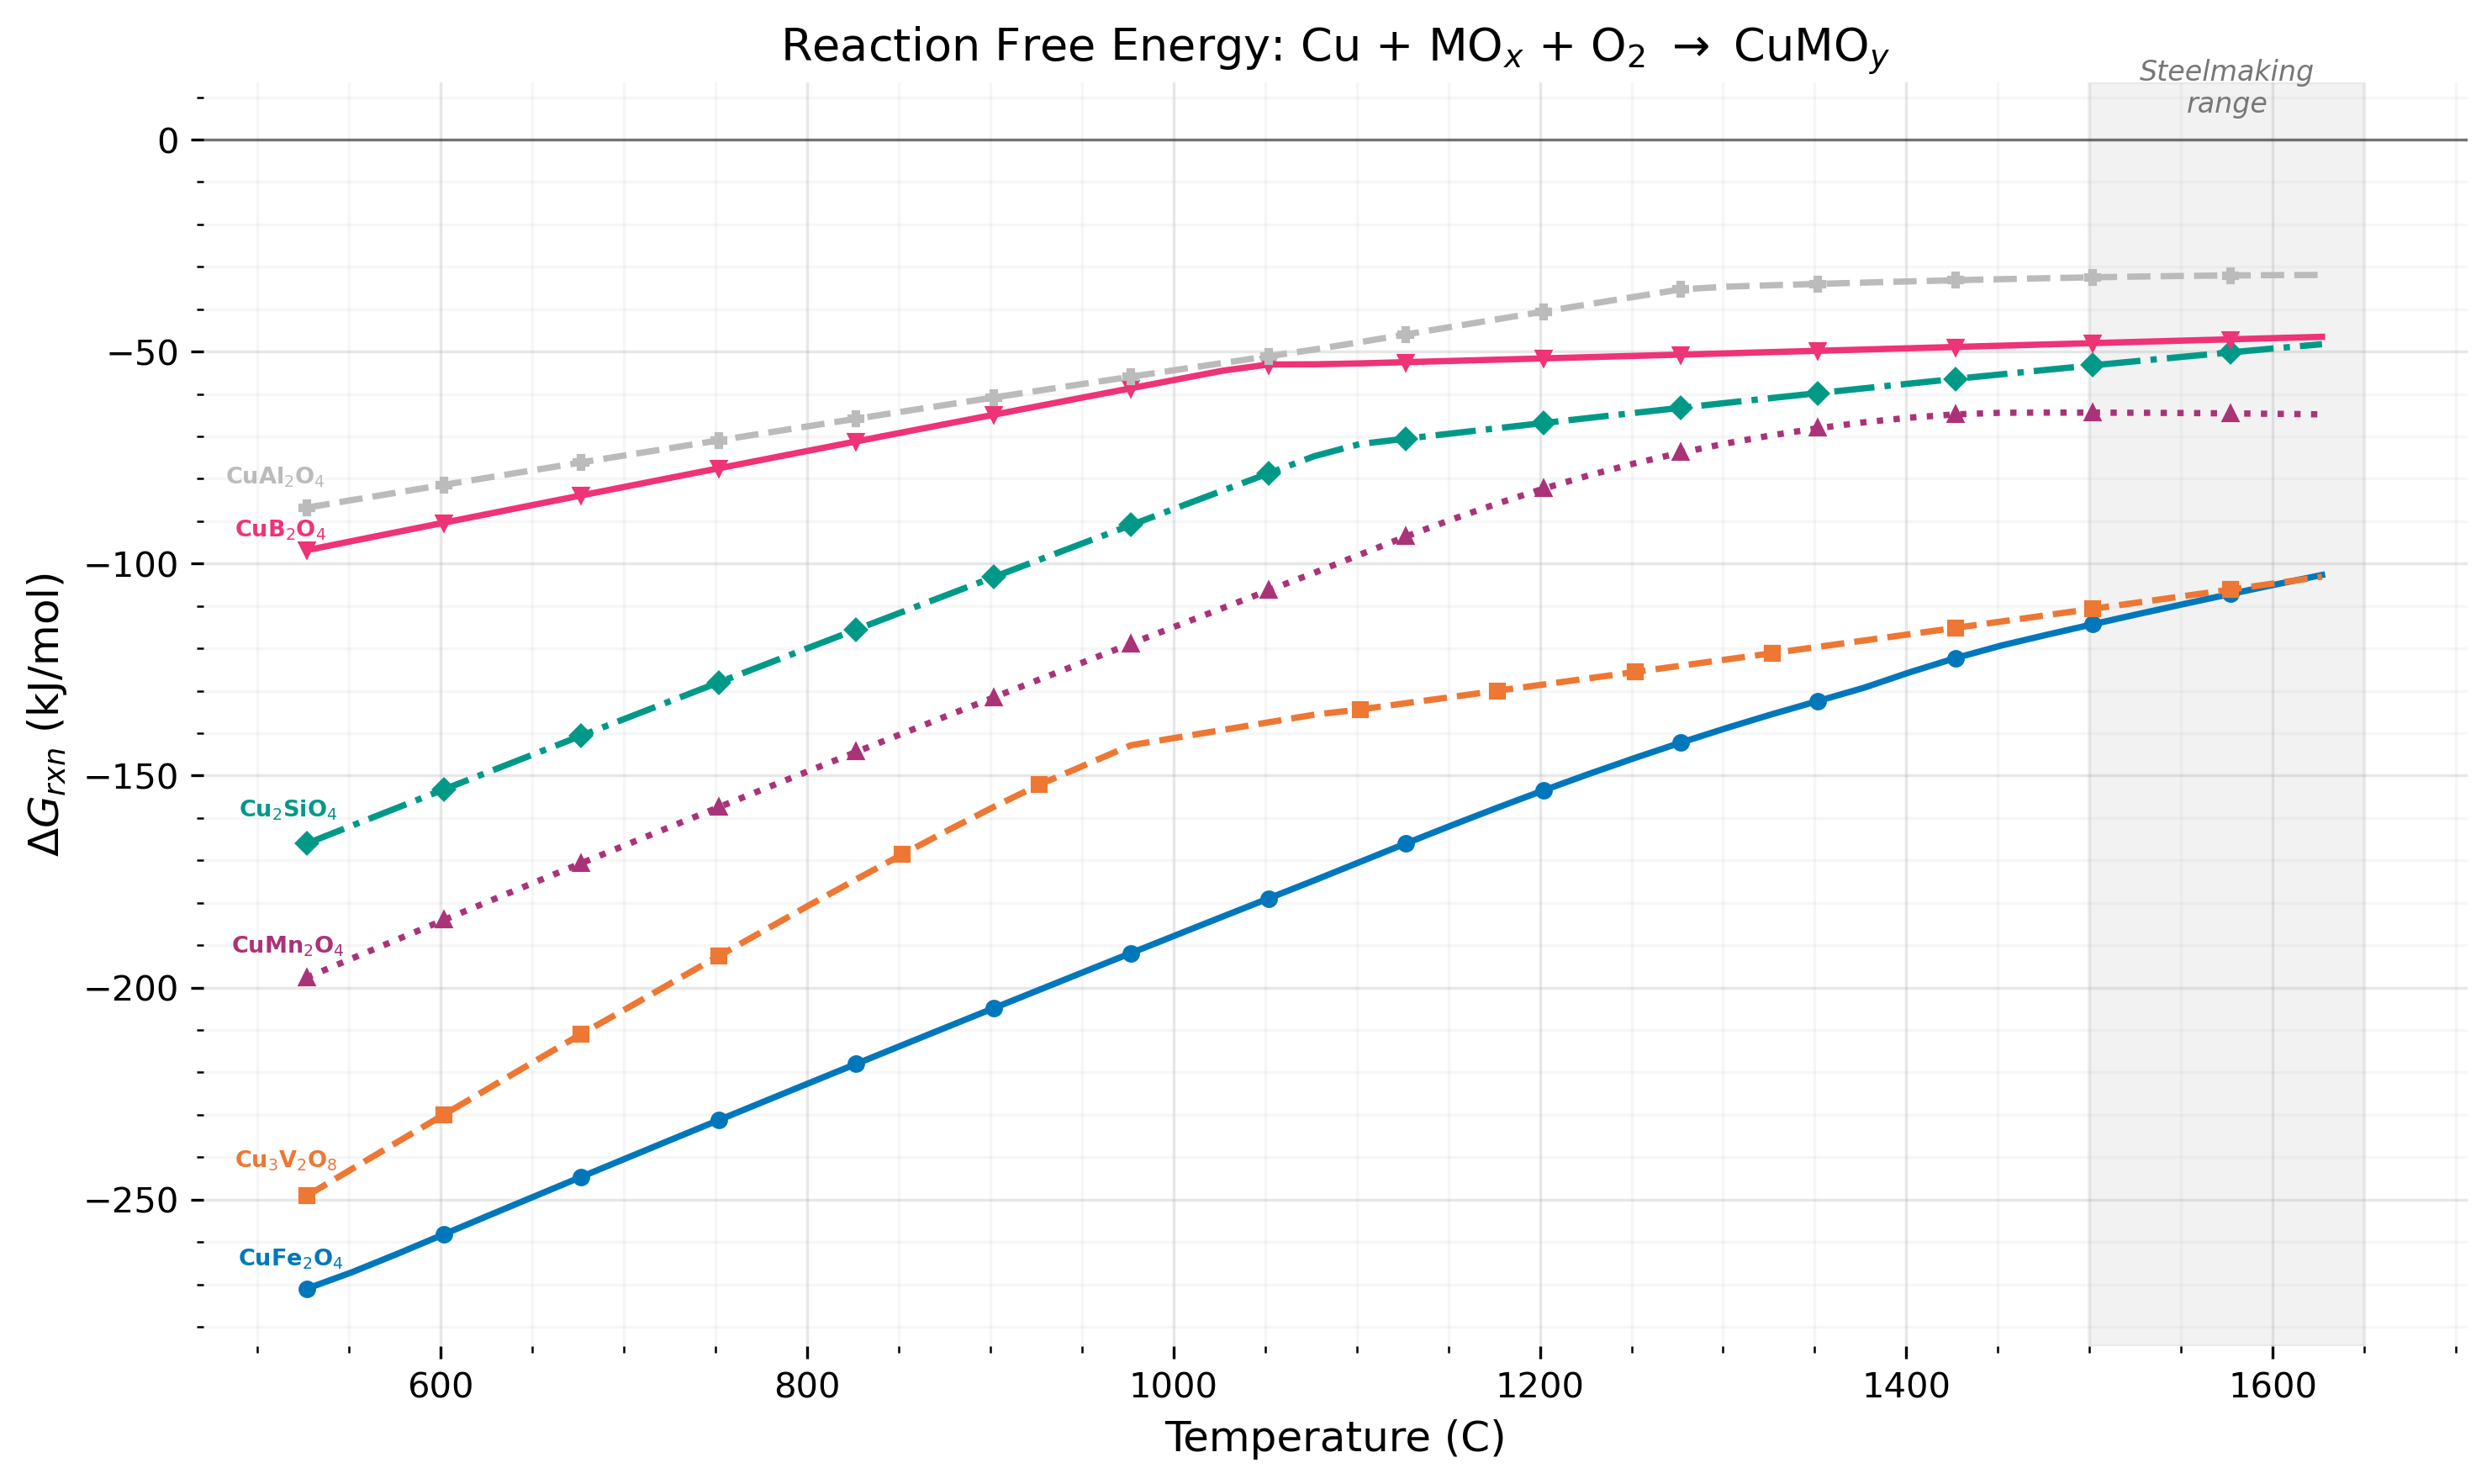
\includegraphics[width=0.85\textwidth]{dG_vs_T_top6.png}
    \caption{$\Delta G$ vs.\ temperature for the top 6 ternary reaction candidates. All reactions become less favorable at higher temperatures, as expected from entropy considerations. Kinks indicate phase transitions (e.g., spinel melting). Script: \texttt{screening/plot\_dG\_vs\_T.py}.}
    \label{fig:dG_vs_T}
\end{figure}

\subsection{Dr.\ Zhang and FeO: Binary vs.\ Ternary}

When asked about FeO, Dr.\ Zhang said:
\begin{quote}
``Iron oxide should not work. I'm pretty sure it doesn't, but I'm not certain.''
\end{quote}

He was talking about the \textbf{binary} reaction (Cu reducing FeO), which is correct; that does not work. Our calculations show a different reaction entirely: Cu $+$ 2FeO $+$ O$_2 \to$ CuFe$_2$O$_4$ (spinel formation). This \textbf{ternary} reaction has the strongest driving force of any candidate ($-112$ kJ). Dr.\ Zhang himself asked us to check it.


%%%%%%%%%%%%%%%%%%%%%%%%%%%%%%%%%%%%%%%%%%%%%%%%%%%%%%%%%%%%%%%%%%%%%%%%%%%%%%%
% 5. ACTIVITY CORRECTION
%%%%%%%%%%%%%%%%%%%%%%%%%%%%%%%%%%%%%%%%%%%%%%%%%%%%%%%%%%%%%%%%%%%%%%%%%%%%%%%
\section{Activity Correction for Dilute Copper}
\label{sec:activity_correction}

\subsection{The Problem with Pure $\Delta G$}

The $\Delta G$ values in Table~\ref{tab:ternary_ranking} assume \textbf{pure Cu} ($a_{\text{Cu}} = 1$). In recycled steel, Cu is dilute: $x_{\text{Cu}} \approx 0.003$ (0.3 wt\%). Dilute Cu has lower chemical potential~\cite{Gaskell2024}, so it is harder to capture.

\subsection{The Penalty Term}

For each Cu atom consumed, there is an activity correction:
\begin{equation}
    \Delta G_{\text{penalty}} = -RT \ln a_{\text{Cu}} = -RT \ln(\gamma_{\text{Cu}} \cdot x_{\text{Cu}})
    \label{eq:penalty}
\end{equation}

Using $\gamma_{\text{Cu}} = 8.5$ (Raoultian activity coefficient for Cu in liquid Fe at \SI{1800}{\kelvin}, from Hino \& Ito~\cite{Hino2010}; Sigworth \& Elliott~\cite{Sigworth1974} give $\sim$10) and $x_{\text{Cu}} = 0.003$:
\[
    a_{\text{Cu}} = 8.5 \times 0.003 = 0.0255
\]
\[
    \Delta G_{\text{penalty per Cu atom}} = -RT \ln(0.0255) = +\SI{54.9}{\kilo\joule\per\mole} \quad \text{at \SI{1800}{\kelvin}}
\]

The total correction scales with the number of Cu atoms in the product:
\begin{equation}
    \Delta G_{\text{eff}} = \Delta G_{\text{pure}} + n_{\text{Cu}} \times \Delta G_{\text{penalty}}
    \label{eq:dG_eff}
\end{equation}

\subsection{Impact on Candidate Ranking}

\begin{insight}[Activity Correction Reshuffles Everything]
Products with multiple Cu atoms per formula unit get penalized heavily:
\begin{itemize}
    \item CuFe$_2$O$_4$ ($n_{\text{Cu}} = 1$): $-111.9 + 54.9 = \mathbf{-57.0}$ kJ (still strongly favorable)
    \item CuMn$_2$O$_4$ ($n_{\text{Cu}} = 1$): $-64.4 + 54.9 = -9.5$ kJ (marginal)
    \item Cu$_3$V$_2$O$_8$ ($n_{\text{Cu}} = 3$): $-109.2 + 3 \times 54.9 = +55.6$ kJ (\textbf{unfavorable!})
\end{itemize}
The pure-$\Delta G$ \#2 candidate (Cu$_3$V$_2$O$_8$) becomes unfavorable once dilution is accounted for. But V$_2$O$_5$ can also form CuV$_2$O$_6$ ($n_{\text{Cu}} = 1$), which gives $-45.0 + 54.9 = +9.9$ kJ. Uncertain, but not clearly dead. At higher Cu concentrations ($\sim$1 wt\%), the activity penalty shrinks and both V$_2$O$_5$ products could become favorable.
\end{insight}

\begin{figure}[H]
    \centering
    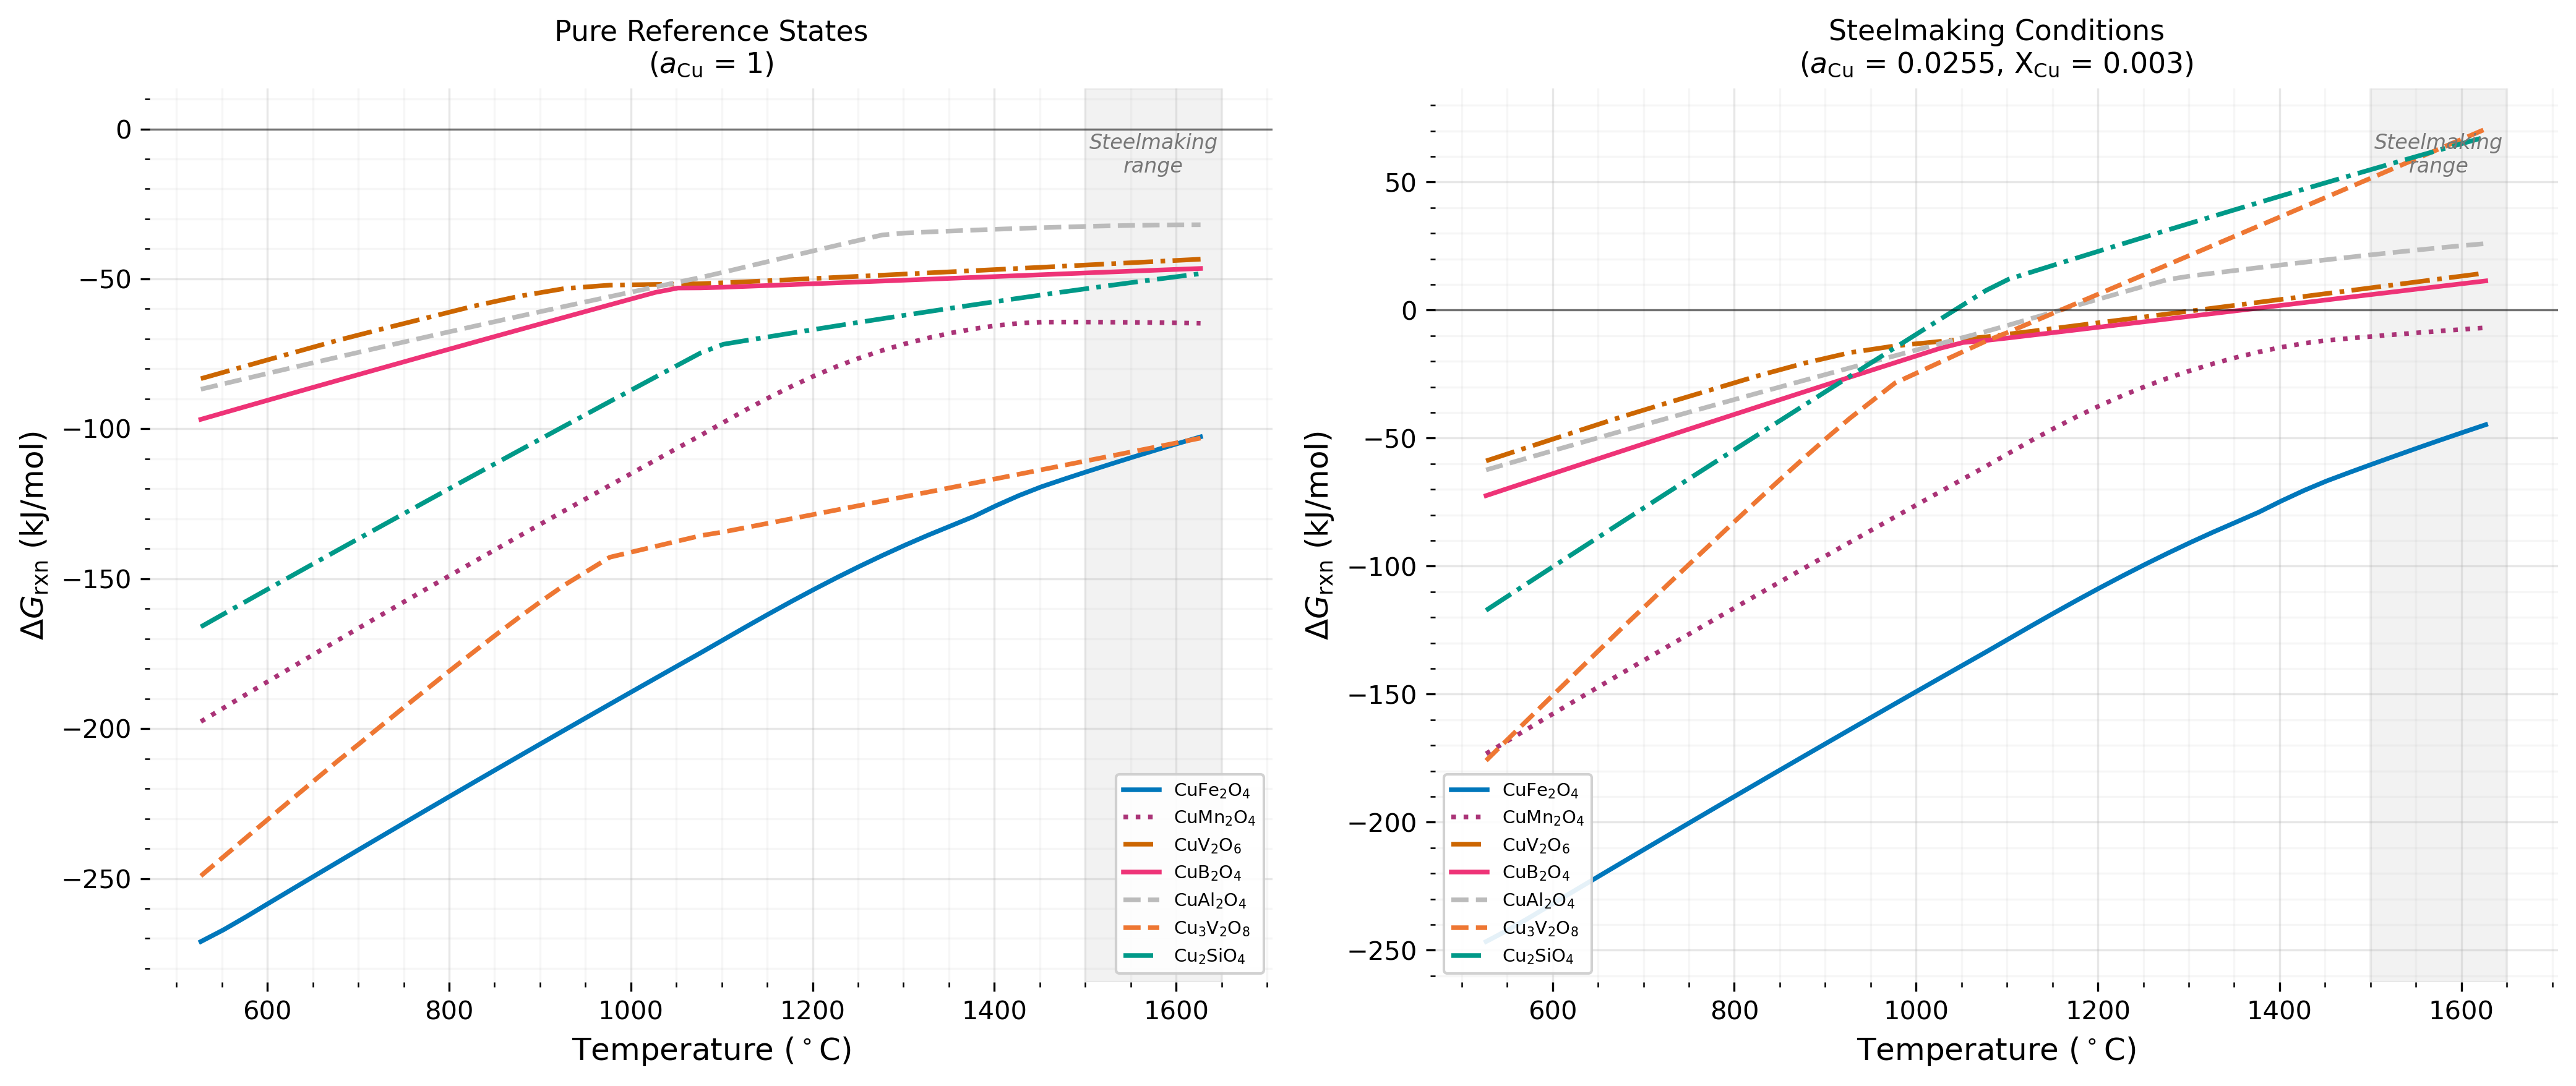
\includegraphics[width=0.85\textwidth]{dG_corrected_comparison.png}
    \caption{Activity-corrected $\Delta G_{\text{eff}}$ vs.\ pure $\Delta G$ for all candidates at \SI{1800}{\kelvin}. Products with $n_{\text{Cu}} \geq 2$ (Cu$_3$V$_2$O$_8$, Cu$_2$SiO$_4$) shift dramatically rightward. Only products to the left of the dashed line ($\Delta G_{\text{eff}} < 0$) are viable under dilute conditions. Script: \texttt{screening/compute\_activity\_corrected\_dG.py}.}
    \label{fig:dG_corrected}
\end{figure}

\subsection{$\gamma_{\text{Cu}}$ Sensitivity}

The literature range for $\gamma_{\text{Cu}}$ is roughly 5--13~\cite{Hino2010, Sigworth1974}. This shifts the penalty by about $\pm 10$ kJ:

\begin{itemize}[leftmargin=*]
    \item CuFe$_2$O$_4$ is \textbf{favorable} across all $\gamma_{\text{Cu}}$ values (always $< -40$ kJ)
    \item CuMn$_2$O$_4$ crosses zero at $\gamma_{\text{Cu}} \approx 5$ (marginal)
    \item CuB$_2$O$_4$ and CuV$_2$O$_6$ hover near zero (uncertain)
    \item Everything with $n_{\text{Cu}} \geq 2$ is unfavorable under steelmaking dilution
\end{itemize}

\begin{figure}[H]
    \centering
    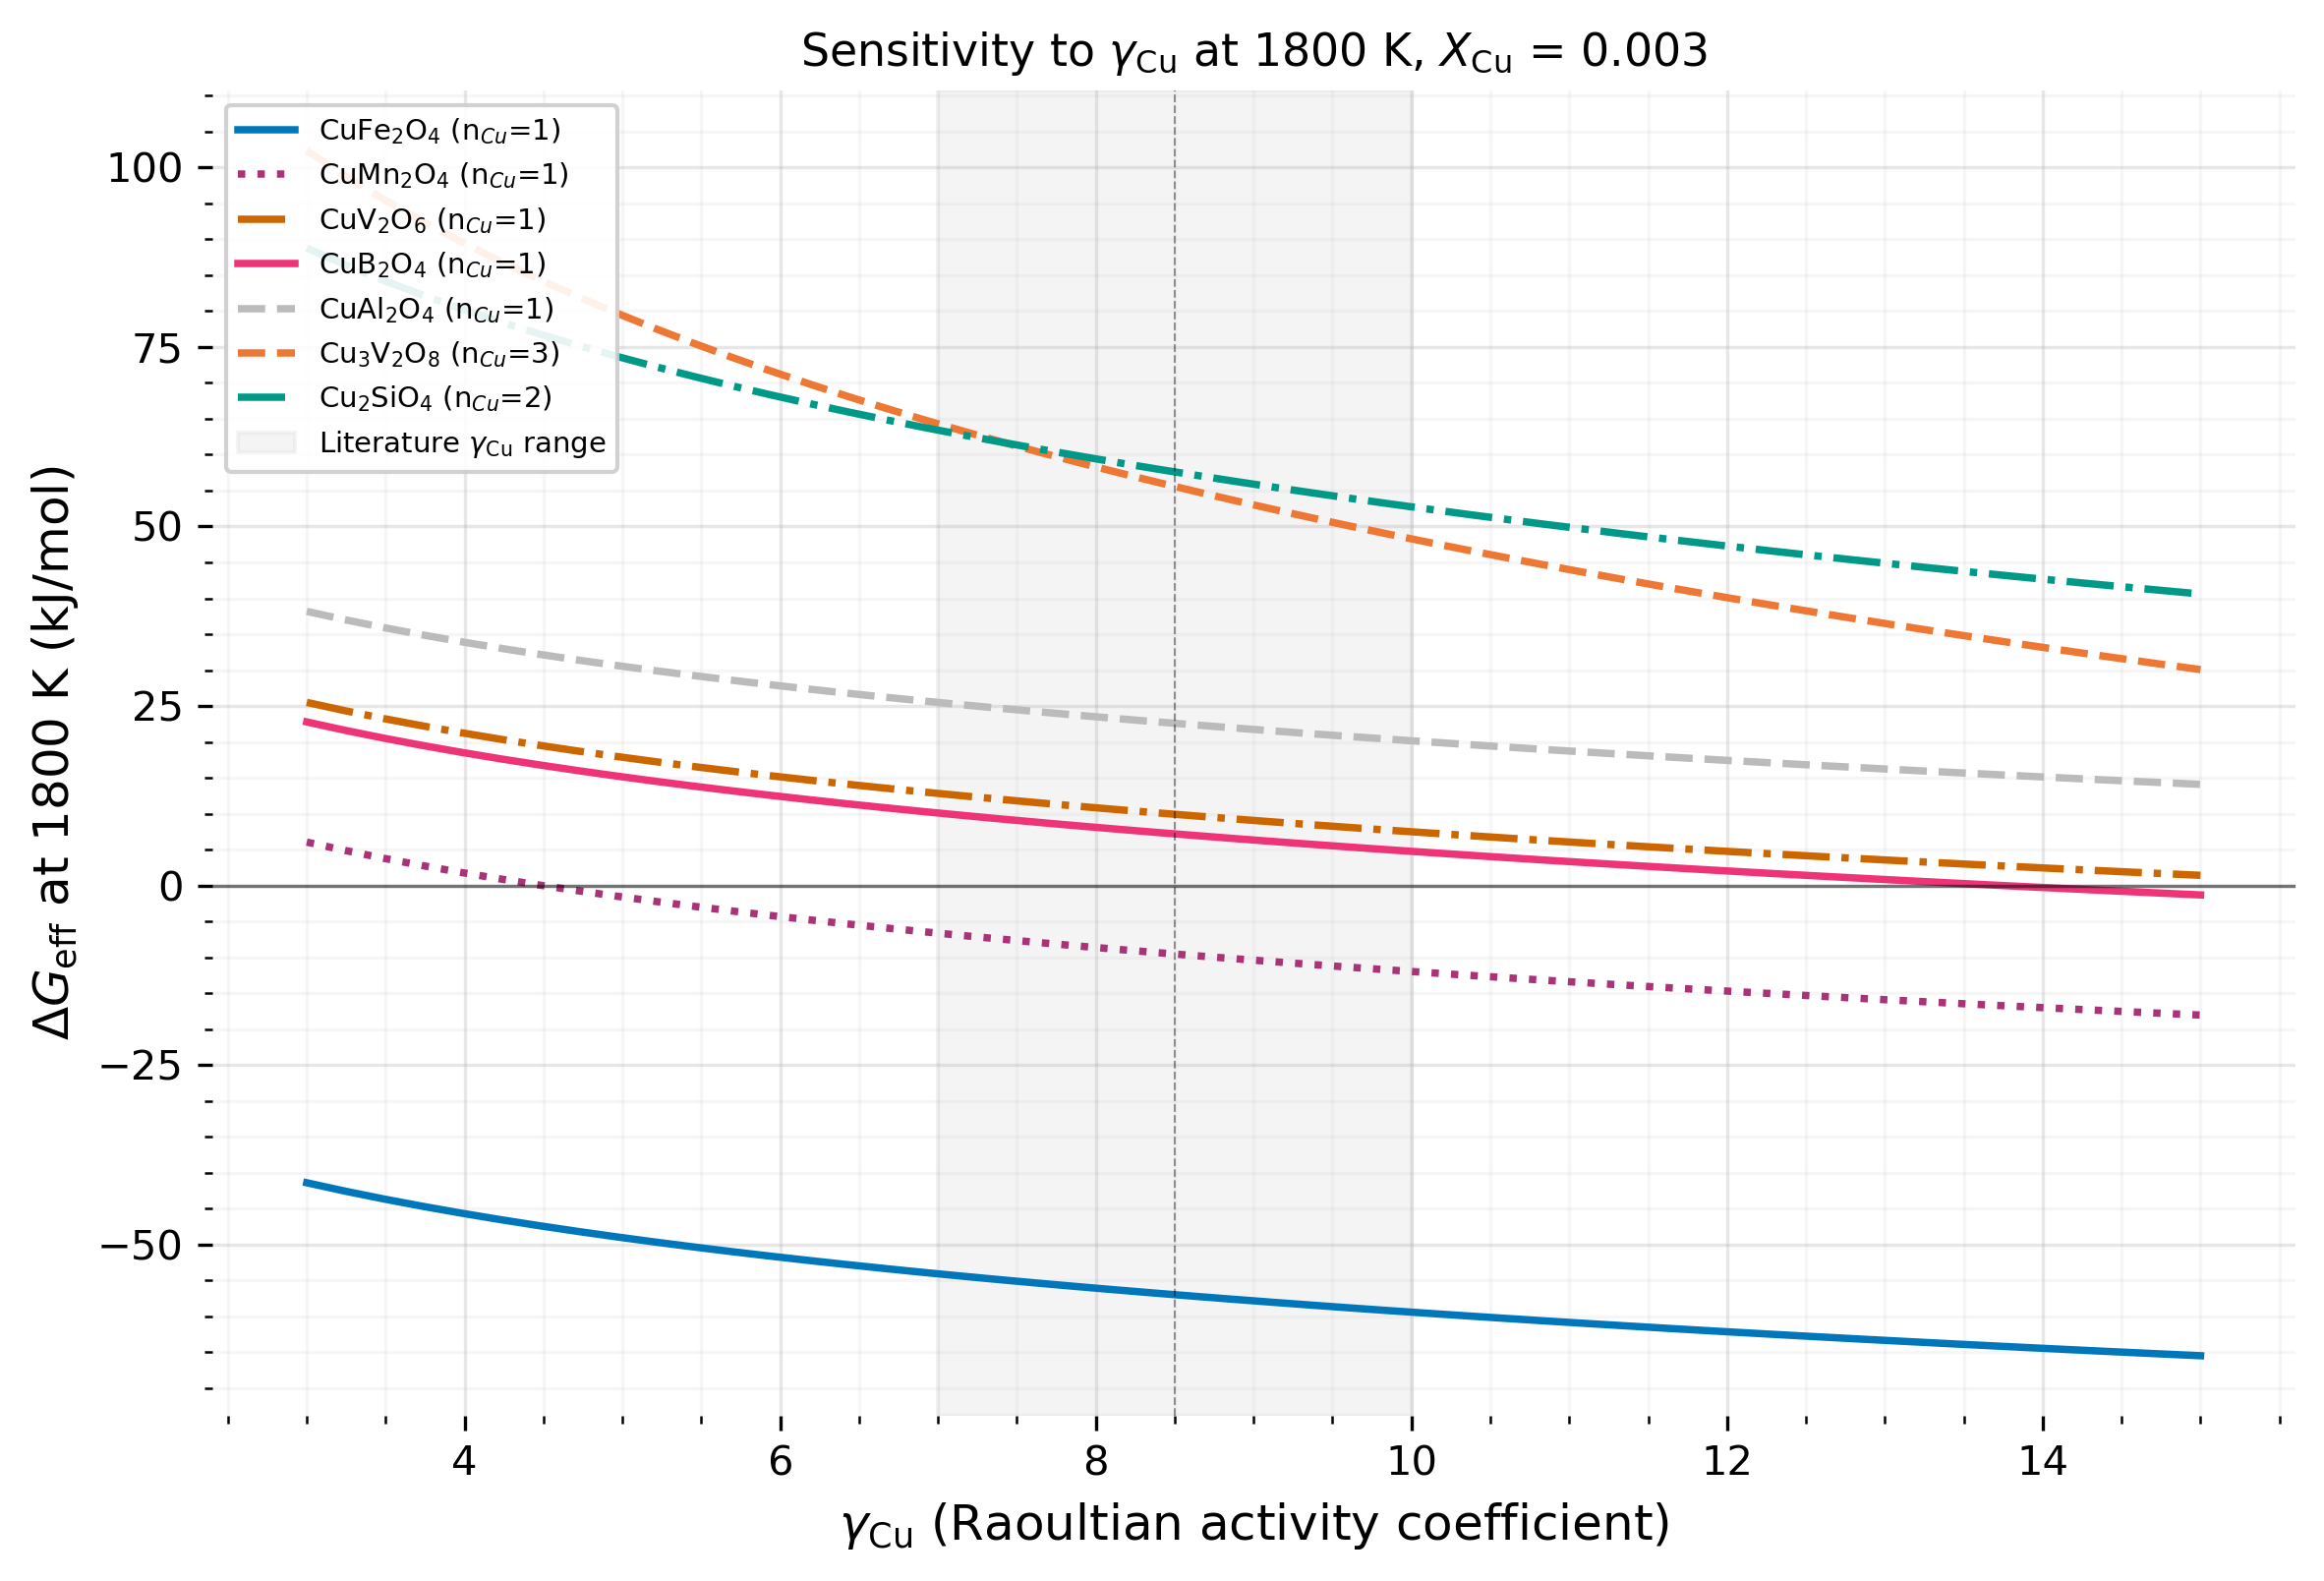
\includegraphics[width=0.85\textwidth]{dG_sensitivity_gamma_Cu.png}
    \caption{Sensitivity of $\Delta G_{\text{eff}}$ to the Cu activity coefficient $\gamma_{\text{Cu}}$ (range 5--13). CuFe$_2$O$_4$ stays favorable across the entire range. CuMn$_2$O$_4$ is marginal. Script: \texttt{screening/compute\_activity\_corrected\_dG.py}.}
    \label{fig:gamma_sensitivity}
\end{figure}


%%%%%%%%%%%%%%%%%%%%%%%%%%%%%%%%%%%%%%%%%%%%%%%%%%%%%%%%%%%%%%%%%%%%%%%%%%%%%%%
% 6. PHASE PERSISTENCE AND SLAG CHEMISTRY
%%%%%%%%%%%%%%%%%%%%%%%%%%%%%%%%%%%%%%%%%%%%%%%%%%%%%%%%%%%%%%%%%%%%%%%%%%%%%%%
\section{Phase Persistence and Slag Chemistry}

\subsection{No Ternary Phase Survives at \SI{1800}{\kelvin}}

A critical finding: while the ternary reactions are thermodynamically favorable, \textbf{no crystalline ternary compound exists at steelmaking temperature}. All named phases (spinels, delafossites, vanadates) melt below \SI{1800}{\kelvin}:

\begin{itemize}[leftmargin=*]
    \item CuFe$_2$O$_4$ spinel: stable to \SI{1700}{\kelvin} (\SI{1427}{\celsius}), closest to steelmaking
    \item CuMn$_2$O$_4$ spinel: stable to \SI{1700}{\kelvin}
    \item CuAl$_2$O$_4$ spinel: stable to \SI{1550}{\kelvin} (\SI{1277}{\celsius})
    \item CuCr$_2$O$_4$ spinel: stable to \SI{1450}{\kelvin}
    \item All other products: always liquid (IONIC\_LIQ in TC-Python)
\end{itemize}

\begin{insight}[Cu Capture = Slag Dissolution]
At steelmaking temperatures, copper is not captured into a crystalline compound~\cite{Porter2021}. Instead, it \textbf{dissolves into the oxide slag} (ionic liquid). The negative $\Delta G$ values still represent a real thermodynamic driving force; they describe the energy released when Cu enters the slag phase. The mechanism is dissolution, not precipitation.

This may actually be advantageous for experiments: a liquid slag has much better contact with molten steel than a solid particle would.
\end{insight}

\subsection{The Ionic Liquid Model in TCOX14}

TCOX14~\cite{TCOX14} models oxide melts using the \textbf{IONIC\_LIQ} phase, a two-sublattice model developed by Hillert et al.~\cite{Hillert2007}: one sublattice holds cations (Cu$^{1+}$, Cu$^{2+}$, Fe$^{2+}$, Fe$^{3+}$, Al$^{3+}$, etc.) and the other holds anions (O$^{2-}$, vacancies, neutral species like SiO$_2$). The excess Gibbs energy captures pairwise interactions between ions on each sublattice. This is how TC-Python knows that Cu prefers certain anion arrangements (like a spinel-like local environment) even when the bulk phase is liquid.

\subsection{Slag Basicity: The Oxide ``Ionic Atmosphere''}
\label{sec:ionic_atmosphere}

If you have done any aqueous solution chemistry, this will feel familiar.

\subsubsection{The Aqueous Analogy}

In aqueous solutions (e.g., OLI simulations with CaCl$_2$, NaCl, KCl), the ions around a dissolved species modify its effective activity~\cite{Gaskell2024}. Adding more salt increases ionic strength, which changes what dissolves and what precipitates. Debye-H\"uckel theory describes this. Order of addition can matter too, because local supersaturation at the mixing point can nucleate different solids before the system reaches equilibrium.

\subsubsection{The Slag Equivalent}

In molten oxide slags, the analogous variable is \textbf{slag basicity}: the ratio of basic oxides (CaO, MnO, FeO, Na$_2$O) to acidic oxides (SiO$_2$, Al$_2$O$_3$)~\cite{Seetharaman2005}. Basicity modifies the activity coefficients of everything in the melt, including Cu. Adding CaO (a strong base) to a silicate slag can shift $\gamma_{\text{CuO}_{0.5}}$ significantly, making Cu easier or harder to dissolve. The surrounding Ca$^{2+}$, Fe$^{2+}$, O$^{2-}$ ions modify the effective chemical potential of Cu in the slag, just like ionic strength modifies solute activity in water. Dr.\ Zhang's suggestion of adding Na$_2$S flux is exactly this idea: change the ``ionic atmosphere'' of the slag to improve Cu capture.

\subsubsection{Modeling Approaches Compared}

\begin{table}[H]
\caption{Activity Coefficient Models: Aqueous vs.\ Oxide Melts}
\label{tab:models_compared}
\centering
\renewcommand{\arraystretch}{1.3}
\begin{tabular}{|>{\raggedright\arraybackslash}p{1.6in}|>{\raggedright\arraybackslash}p{2.1in}|>{\raggedright\arraybackslash}p{2.1in}|}
\hline
\rowcolor{headercolor}
\textcolor{white}{\textbf{Feature}} & \textcolor{white}{\textbf{Aqueous (OLI)}} & \textcolor{white}{\textbf{Oxide Slag (TCOX14)}} \\
\hline
Model & MSE (Mixed Solvent Electrolyte) & Ionic Two-Sublattice \\
\hline
\rowcolor{altrow}
Core concept & Excess $G$ from pairwise ion interactions & Excess $G$ from pairwise ion interactions \\
\hline
Reference state & Infinite dilution in water & Pure oxide liquid \\
\hline
\rowcolor{altrow}
Temperature range & 25--\SI{300}{\celsius} & 1200--\SI{1800}{\celsius} \\
\hline
Key variable & Ionic strength & Slag basicity \\
\hline
\rowcolor{altrow}
Software & OLI Studio & Thermo-Calc (TCOX14) \\
\hline
Competing approach & Pitzer model & Modified Quasichemical Model (FactSage) \\
\hline
\end{tabular}
\end{table}

The physics is the same in both cases: excess Gibbs energy from pairwise ion interactions determines activity coefficients. The only differences are the solvent (water vs.\ oxide melt) and the temperature range.

FactSage uses the Modified Quasichemical Model (MQM) instead of the two-sublattice approach. Some slag chemists prefer MQM because it handles short-range ordering in silicate melts better~\cite{Seetharaman2005}. In practice, both are fitted to the same experimental data and give similar results for most systems.

\subsubsection{Thermodynamics vs.\ Kinetics of Mixing}

\textbf{Thermodynamically}, the final slag composition determines equilibrium regardless of mixing order. Gibbs energy reaches the same minimum either way~\cite{Gaskell2024}.

\textbf{Kinetically}, order matters. If you dump MnO into a silicate slag, local supersaturation at the addition point can nucleate MnSiO$_3$ crystals before the system mixes. Those metastable precipitates might trap or release Cu differently than the equilibrium slag would. Modeling these transient gradients is a \textbf{DICTRA problem}~\cite{Andersson2002}: you need diffusion simulation, not just equilibrium thermo.

\subsection{Slag Basicity Results}

Script~5 (\texttt{slag\_composition\_effects.py}) tested two quaternary systems at \SI{1800}{\kelvin}. In Cu-Mn-Si-O, increasing the MnO:SiO$_2$ ratio \textit{decreases} $a_{\text{Cu}}$ by 17\%, meaning a more basic slag captures Cu more effectively. That is a tunable parameter for experiments. In Cu-Al-Si-O, varying Al$_2$O$_3$:SiO$_2$ has almost no effect on $a_{\text{Cu}}$; the alumina is essentially inert as far as Cu activity goes.

A real steelmaking slag is CaO-SiO$_2$-Al$_2$O$_3$-FeO-MnO-MgO. Future work should explore quinary and higher-order systems (e.g., Cu-Fe-Mn-Ca-Si-O) to map how basicity affects Cu capture in realistic compositions.

\begin{figure}[H]
    \centering
    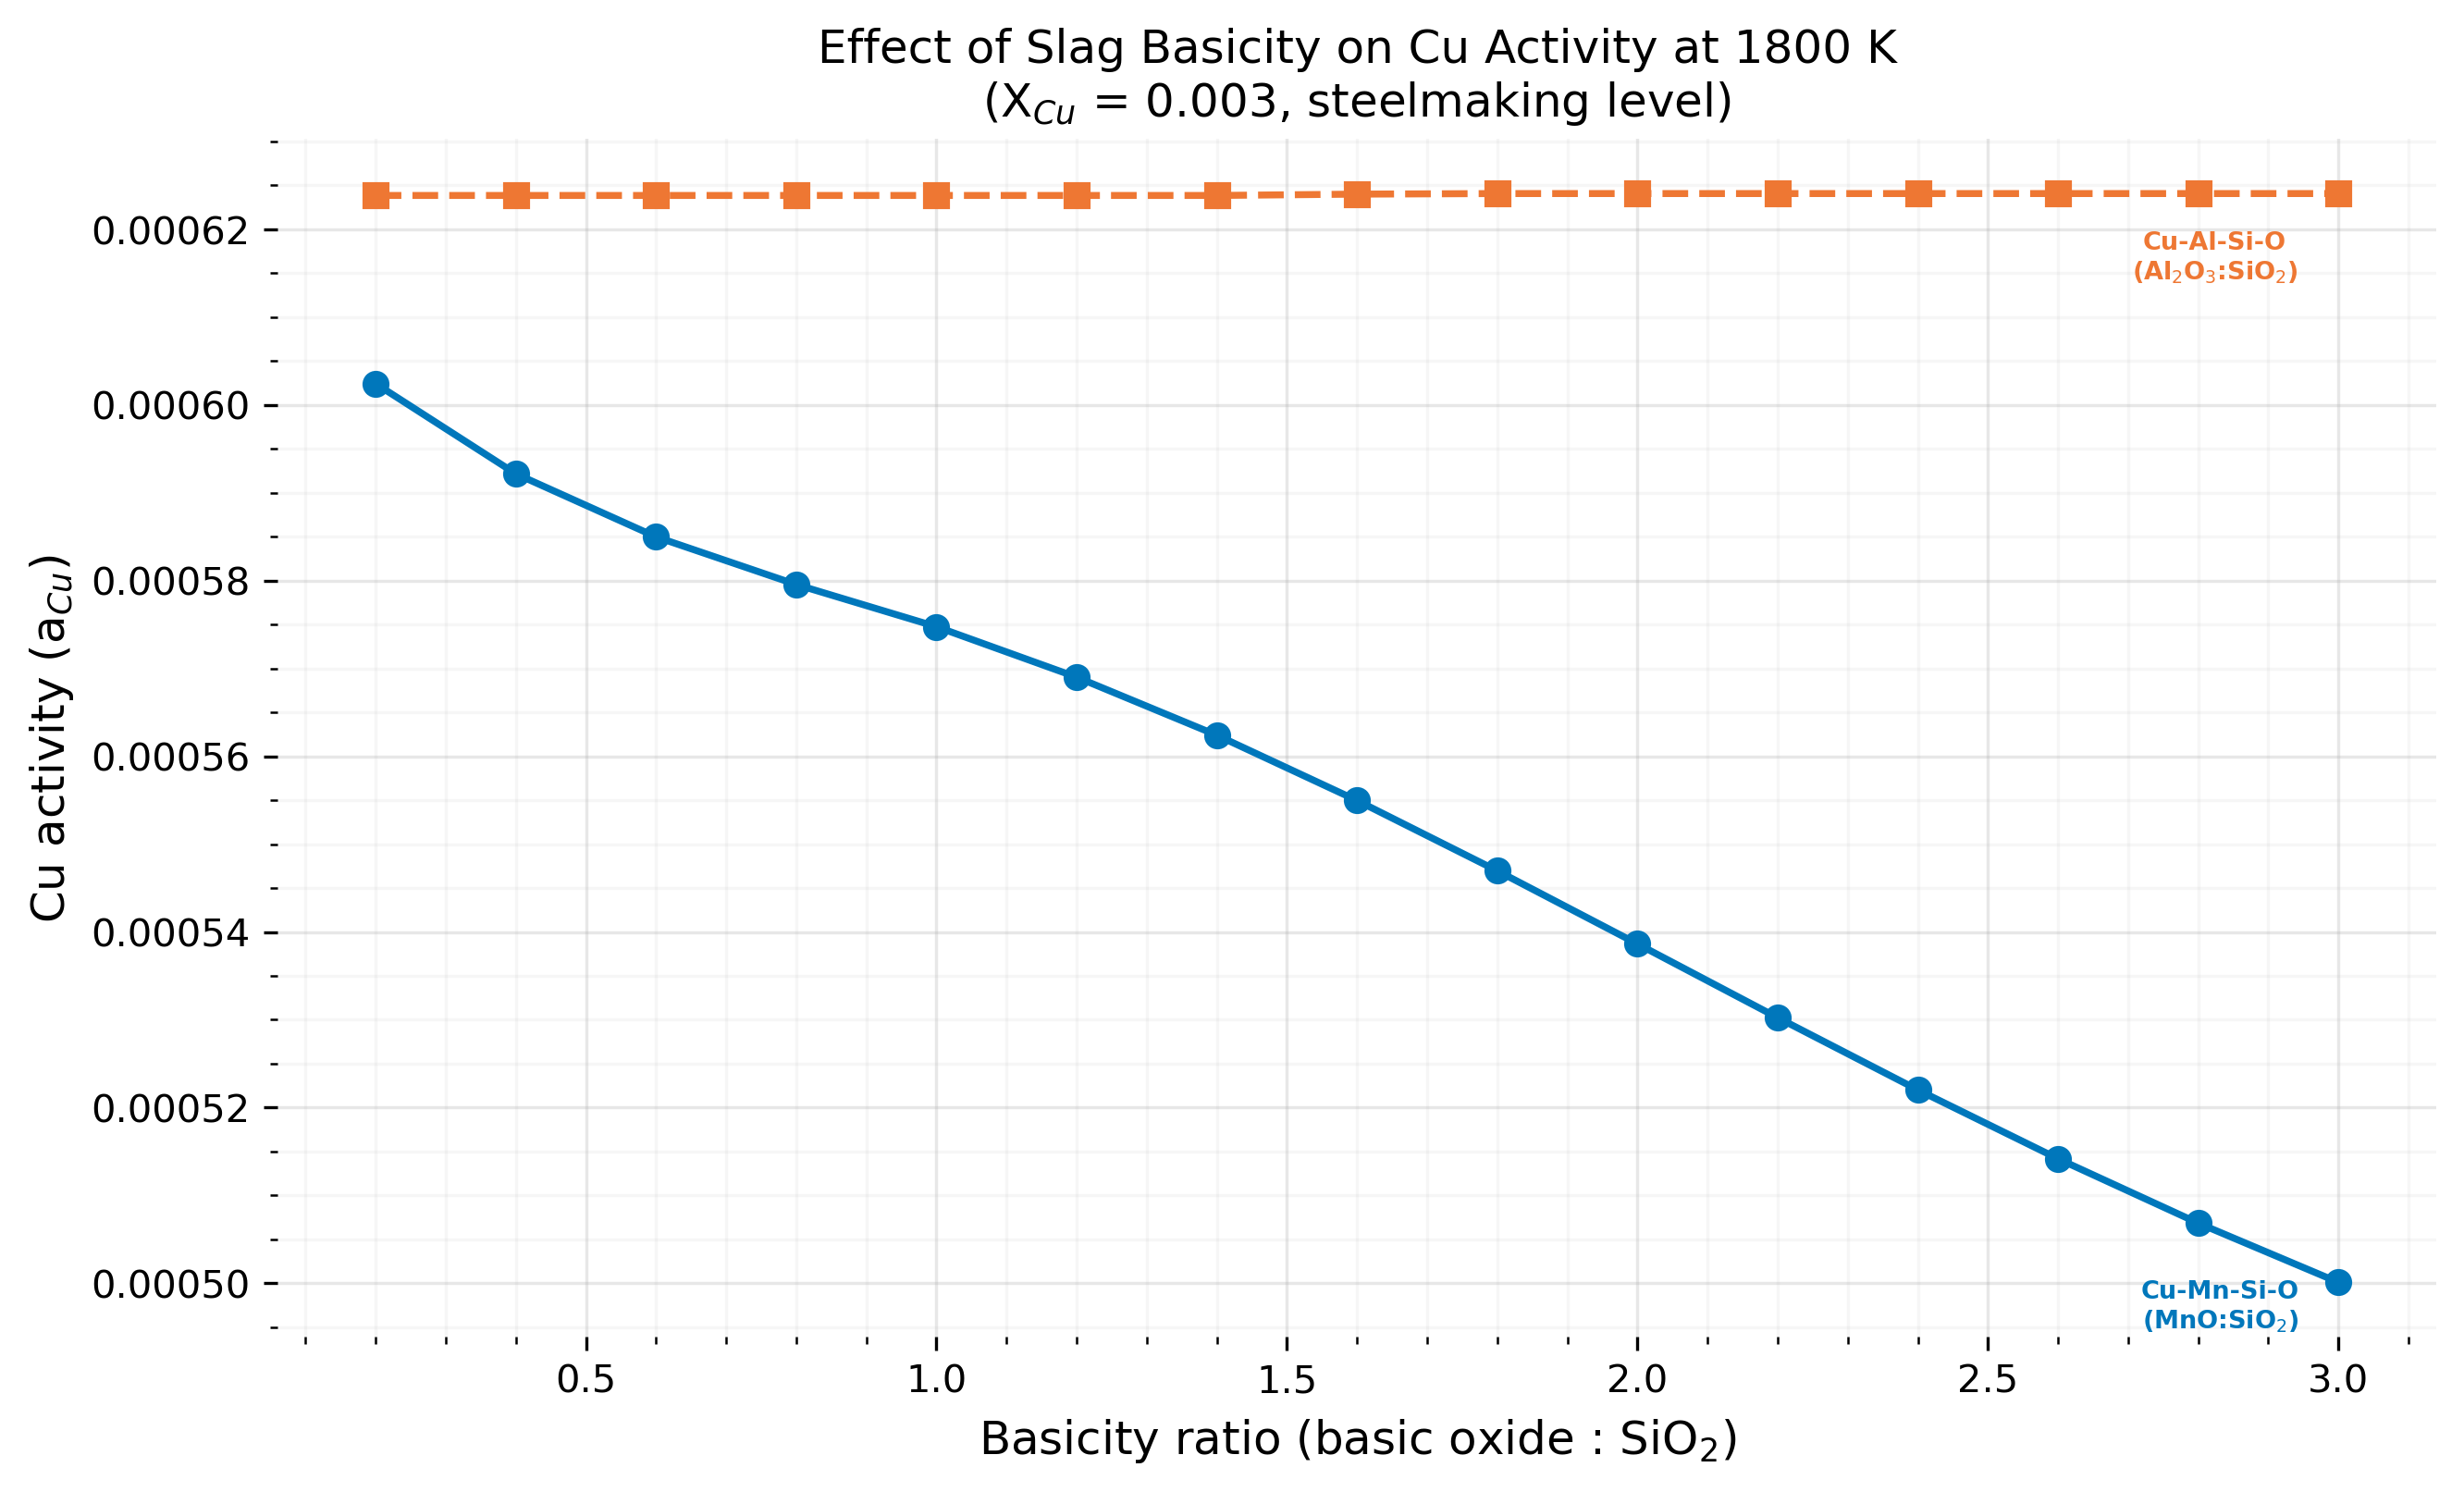
\includegraphics[width=0.85\textwidth]{slag_basicity_vs_aCu.png}
    \caption{Cu activity vs.\ slag basicity ratio for Cu-Mn-Si-O and Cu-Al-Si-O at \SI{1800}{\kelvin}. Increasing MnO:SiO$_2$ (more basic) reduces $a_{\text{Cu}}$ by 17\%, while Al$_2$O$_3$:SiO$_2$ has negligible effect. Script: \texttt{screening/plot\_slag\_effects.py}.}
    \label{fig:slag_basicity}
\end{figure}


%%%%%%%%%%%%%%%%%%%%%%%%%%%%%%%%%%%%%%%%%%%%%%%%%%%%%%%%%%%%%%%%%%%%%%%%%%%%%%%
% 7. Cu ACTIVITY AND GIBBS PHASE RULE
%%%%%%%%%%%%%%%%%%%%%%%%%%%%%%%%%%%%%%%%%%%%%%%%%%%%%%%%%%%%%%%%%%%%%%%%%%%%%%%
\section{Cu Activity and the Gibbs Phase Rule}

\subsection{The ``Flat Activity'' Puzzle}

Script~2 (\texttt{cu\_activity\_vs\_oxide.py}) swept Cu mole fraction from 0.90 to 0.05 in four ternary systems at \SI{1800}{\kelvin}, recording $a_{\text{Cu}}$ via \texttt{AC(CU)} in TC-Python. The result was puzzling: $a_{\text{Cu}}$ was essentially \textbf{constant} ($\sim 6 \times 10^{-4}$) across the entire composition range for Cu-Al-O, Cu-Mn-O, and Cu-Fe-O.

\subsection{Explanation: Gibbs Phase Rule}

This is not a code bug. It follows directly from the \textbf{Gibbs Phase Rule}~\cite{Gaskell2024, Brown2026TC1}:
\[
    F = C - P + 2
\]

At fixed $T$ and $P$ ($F$ reduced by 2), for a 3-component system ($C = 3$) in a 2-phase field ($P = 2$):
\[
    F = 3 - 2 + 2 - 2 = 1
\]

But we have already fixed $T$ and $P$, so $F = 1$. In a 2-phase field, the compositions of both phases are \textbf{fixed}; only the relative \textit{amounts} change as you move along a tie line (lever rule). Since phase compositions are fixed, activity is invariant.

\begin{insight}[Why $a_{\text{Cu}}$ Is Flat]
In TCOX14 at \SI{1800}{\kelvin}, most Cu-M-O systems sit in a 2-phase field (e.g., CORUNDUM + IONIC\_LIQ for Cu-Al-O). Sweeping overall composition just moves along the tie line between these two phases without changing either phase's composition. The Cu activity, which depends on the phase compositions (not the overall composition), stays constant.
\end{insight}

\subsection{The Missing Metal Phase}

TCOX14 has \textbf{no separate metallic Cu phase} (no FCC\_A1 or metallic LIQUID). All Cu dissolves into the IONIC\_LIQ (two-sublattice ionic liquid model). This means TCOX14 cannot model the steel/slag interface; it only sees the slag side.

To get $a_{\text{Cu}}$ in metallic Cu coexisting with oxide slag, you would need a database containing \textbf{both} metallic phases (from TCFE) and oxide phases (from TCOX). Whether TCFE13 + TCOX14 can be combined is an open question tied to the DICTRA testing (Section~\ref{sec:dictra}).

\subsection{The $a_{\text{Cu}} \approx 0.0006$ Value}

\begin{figure}[H]
    \centering
    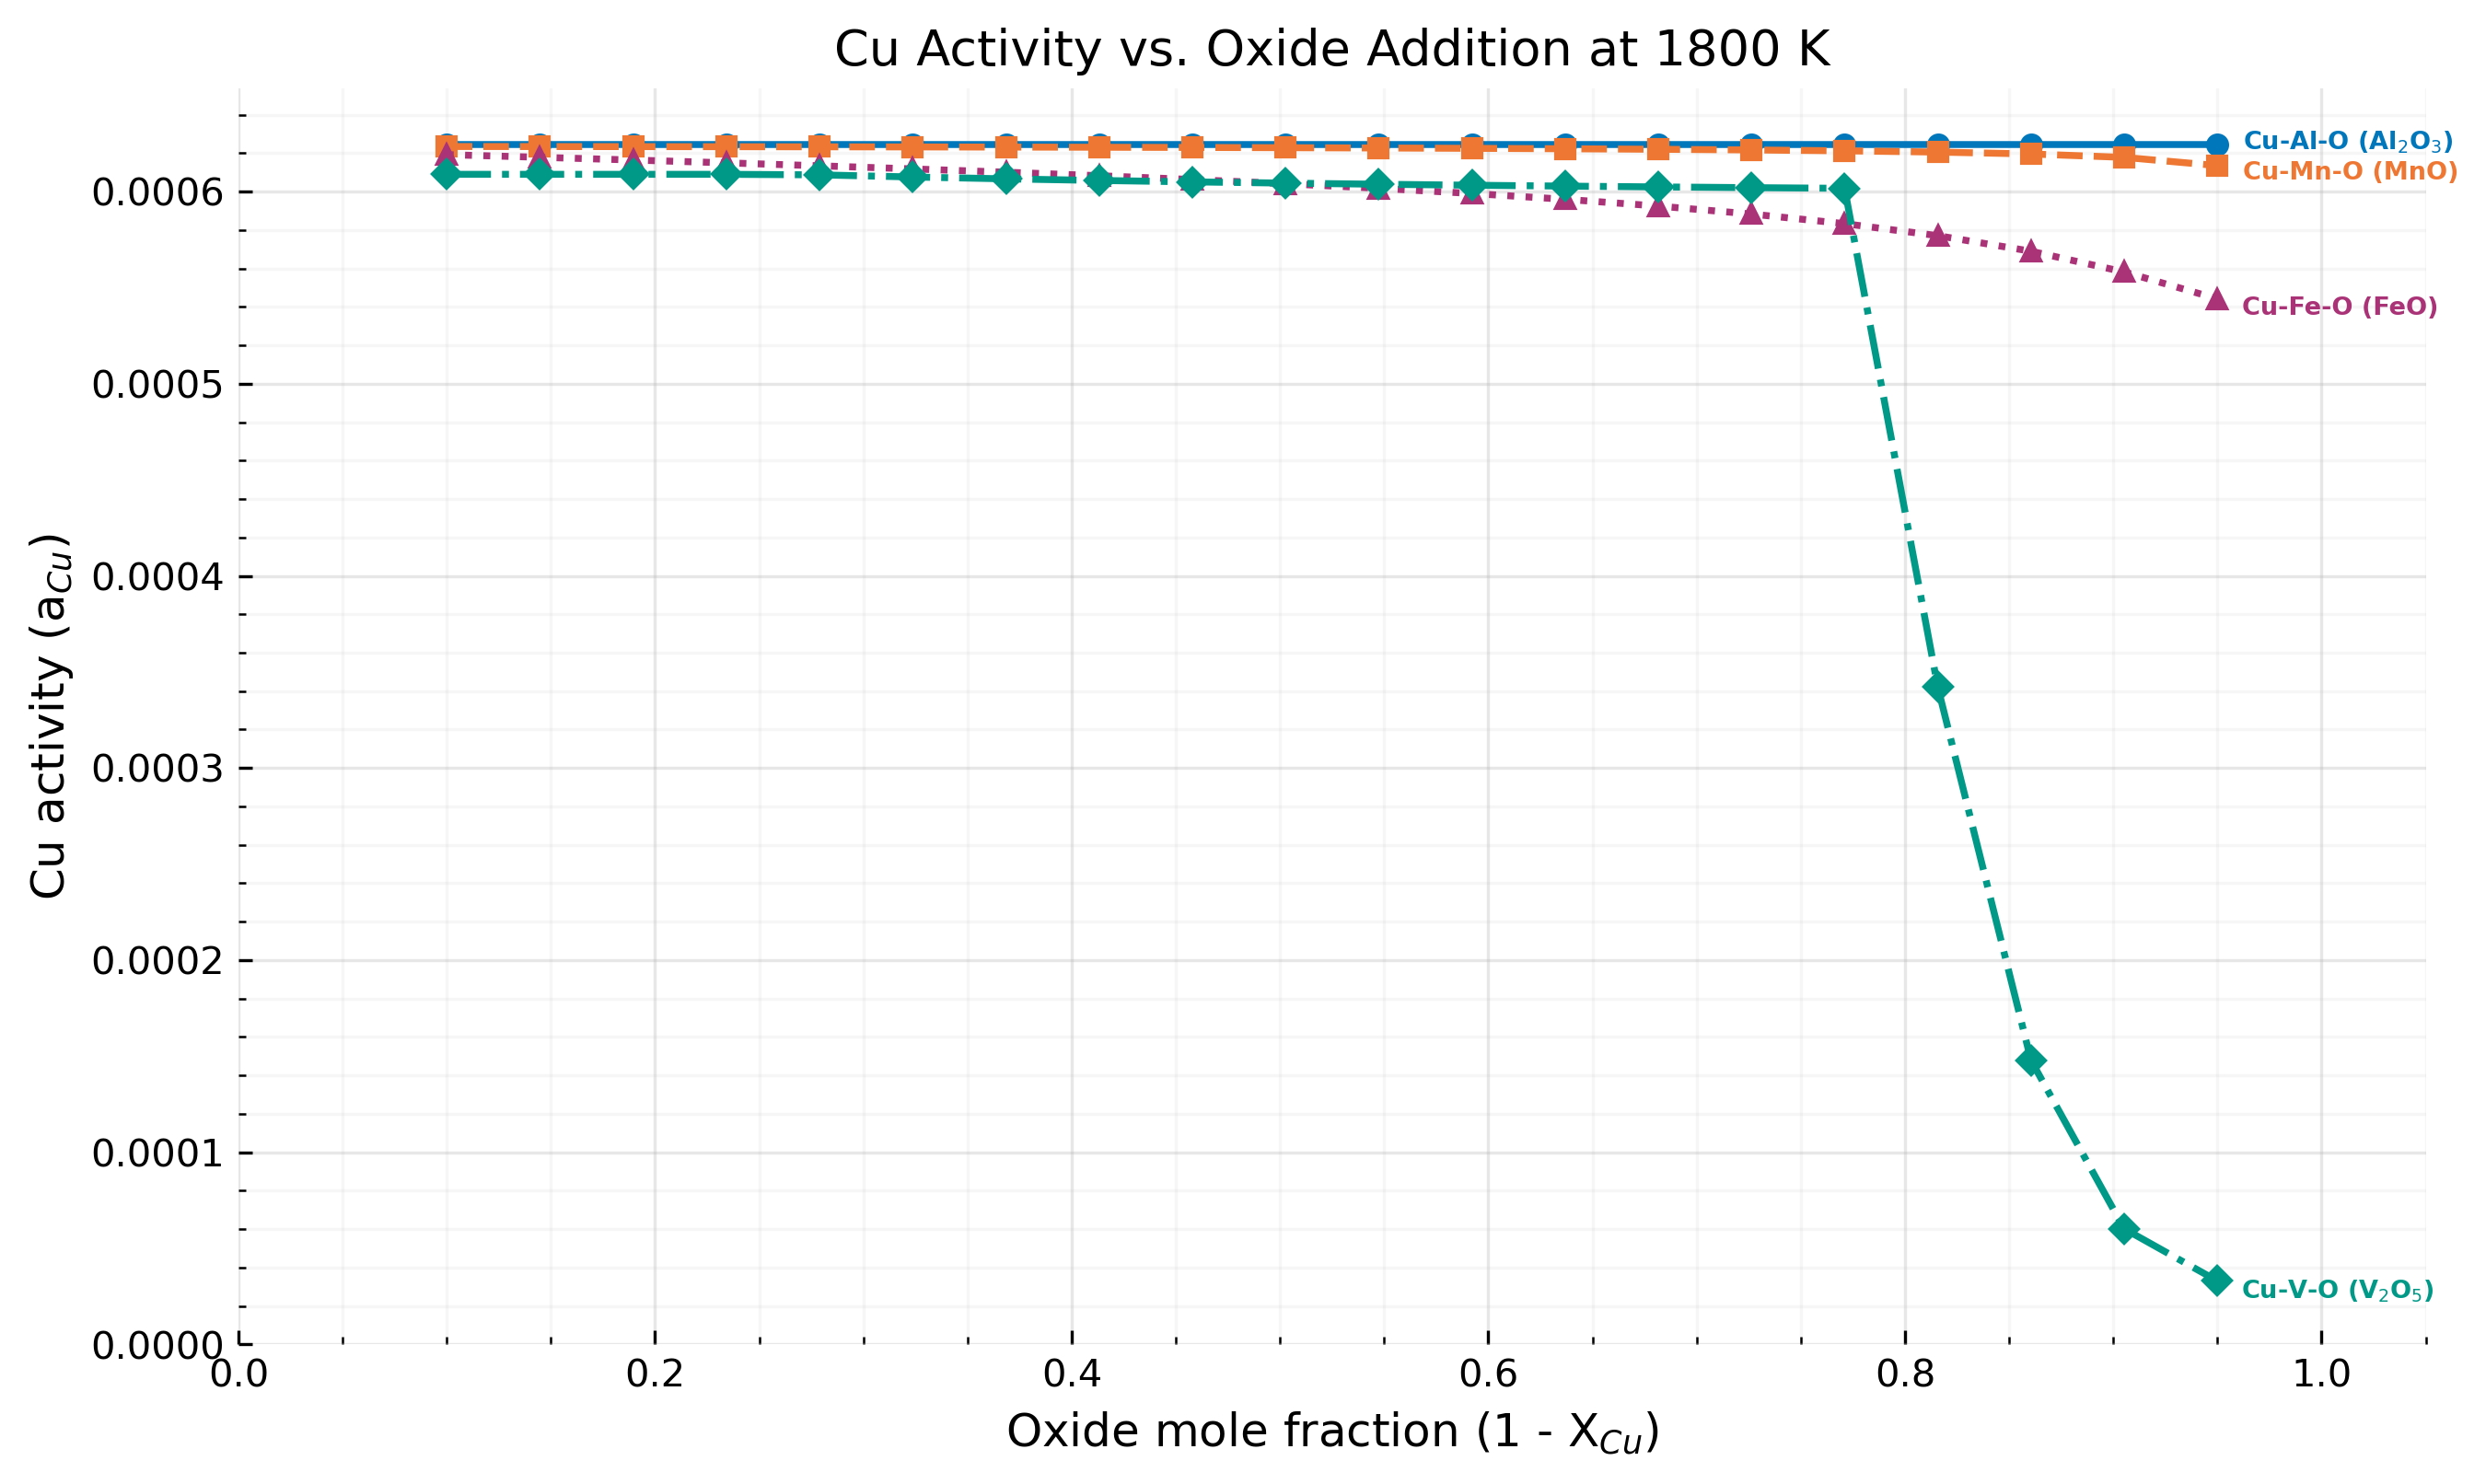
\includegraphics[width=0.85\textwidth]{cu_activity_vs_oxide.png}
    \caption{Cu activity ($a_{\text{Cu}}$) vs.\ mole fraction of Cu in four ternary systems at \SI{1800}{\kelvin}. Activity is flat across the entire sweep for Cu-Al-O, Cu-Mn-O, and Cu-Fe-O (Gibbs Phase Rule: 2-phase field constrains compositions). Cu-V-O shows a drop to $3 \times 10^{-5}$ at high oxide fraction. Script: \texttt{screening/plot\_cu\_activity.py}.}
    \label{fig:cu_activity}
\end{figure}

The flat value of $a_{\text{Cu}} \approx 6 \times 10^{-4}$ \textit{is} physically meaningful. It represents the equilibrium Cu activity set by the Cu-O redox couple in the ionic liquid at \SI{1800}{\kelvin}. In the Cu-V-O system, $a_{\text{Cu}}$ drops further to $\sim 3 \times 10^{-5}$ at high oxide fractions, indicating that V$_2$O$_5$ captures Cu most aggressively among the systems tested.


%%%%%%%%%%%%%%%%%%%%%%%%%%%%%%%%%%%%%%%%%%%%%%%%%%%%%%%%%%%%%%%%%%%%%%%%%%%%%%%
% 7b. TERNARY PHASE MAPS
%%%%%%%%%%%%%%%%%%%%%%%%%%%%%%%%%%%%%%%%%%%%%%%%%%%%%%%%%%%%%%%%%%%%%%%%%%%%%%%
\section{Ternary Phase Maps at \SI{1800}{\kelvin}}
\label{sec:phase_maps}

Script~5 (\texttt{ternary\_phase\_map\_1800K.py}) mapped phase stability across 20$\times$20 composition grids in three Cu-M-O systems at \SI{1800}{\kelvin}. These maps reveal which phases dominate at steelmaking temperature and confirm that most of the composition space is molten.

\begin{figure}[H]
    \centering
    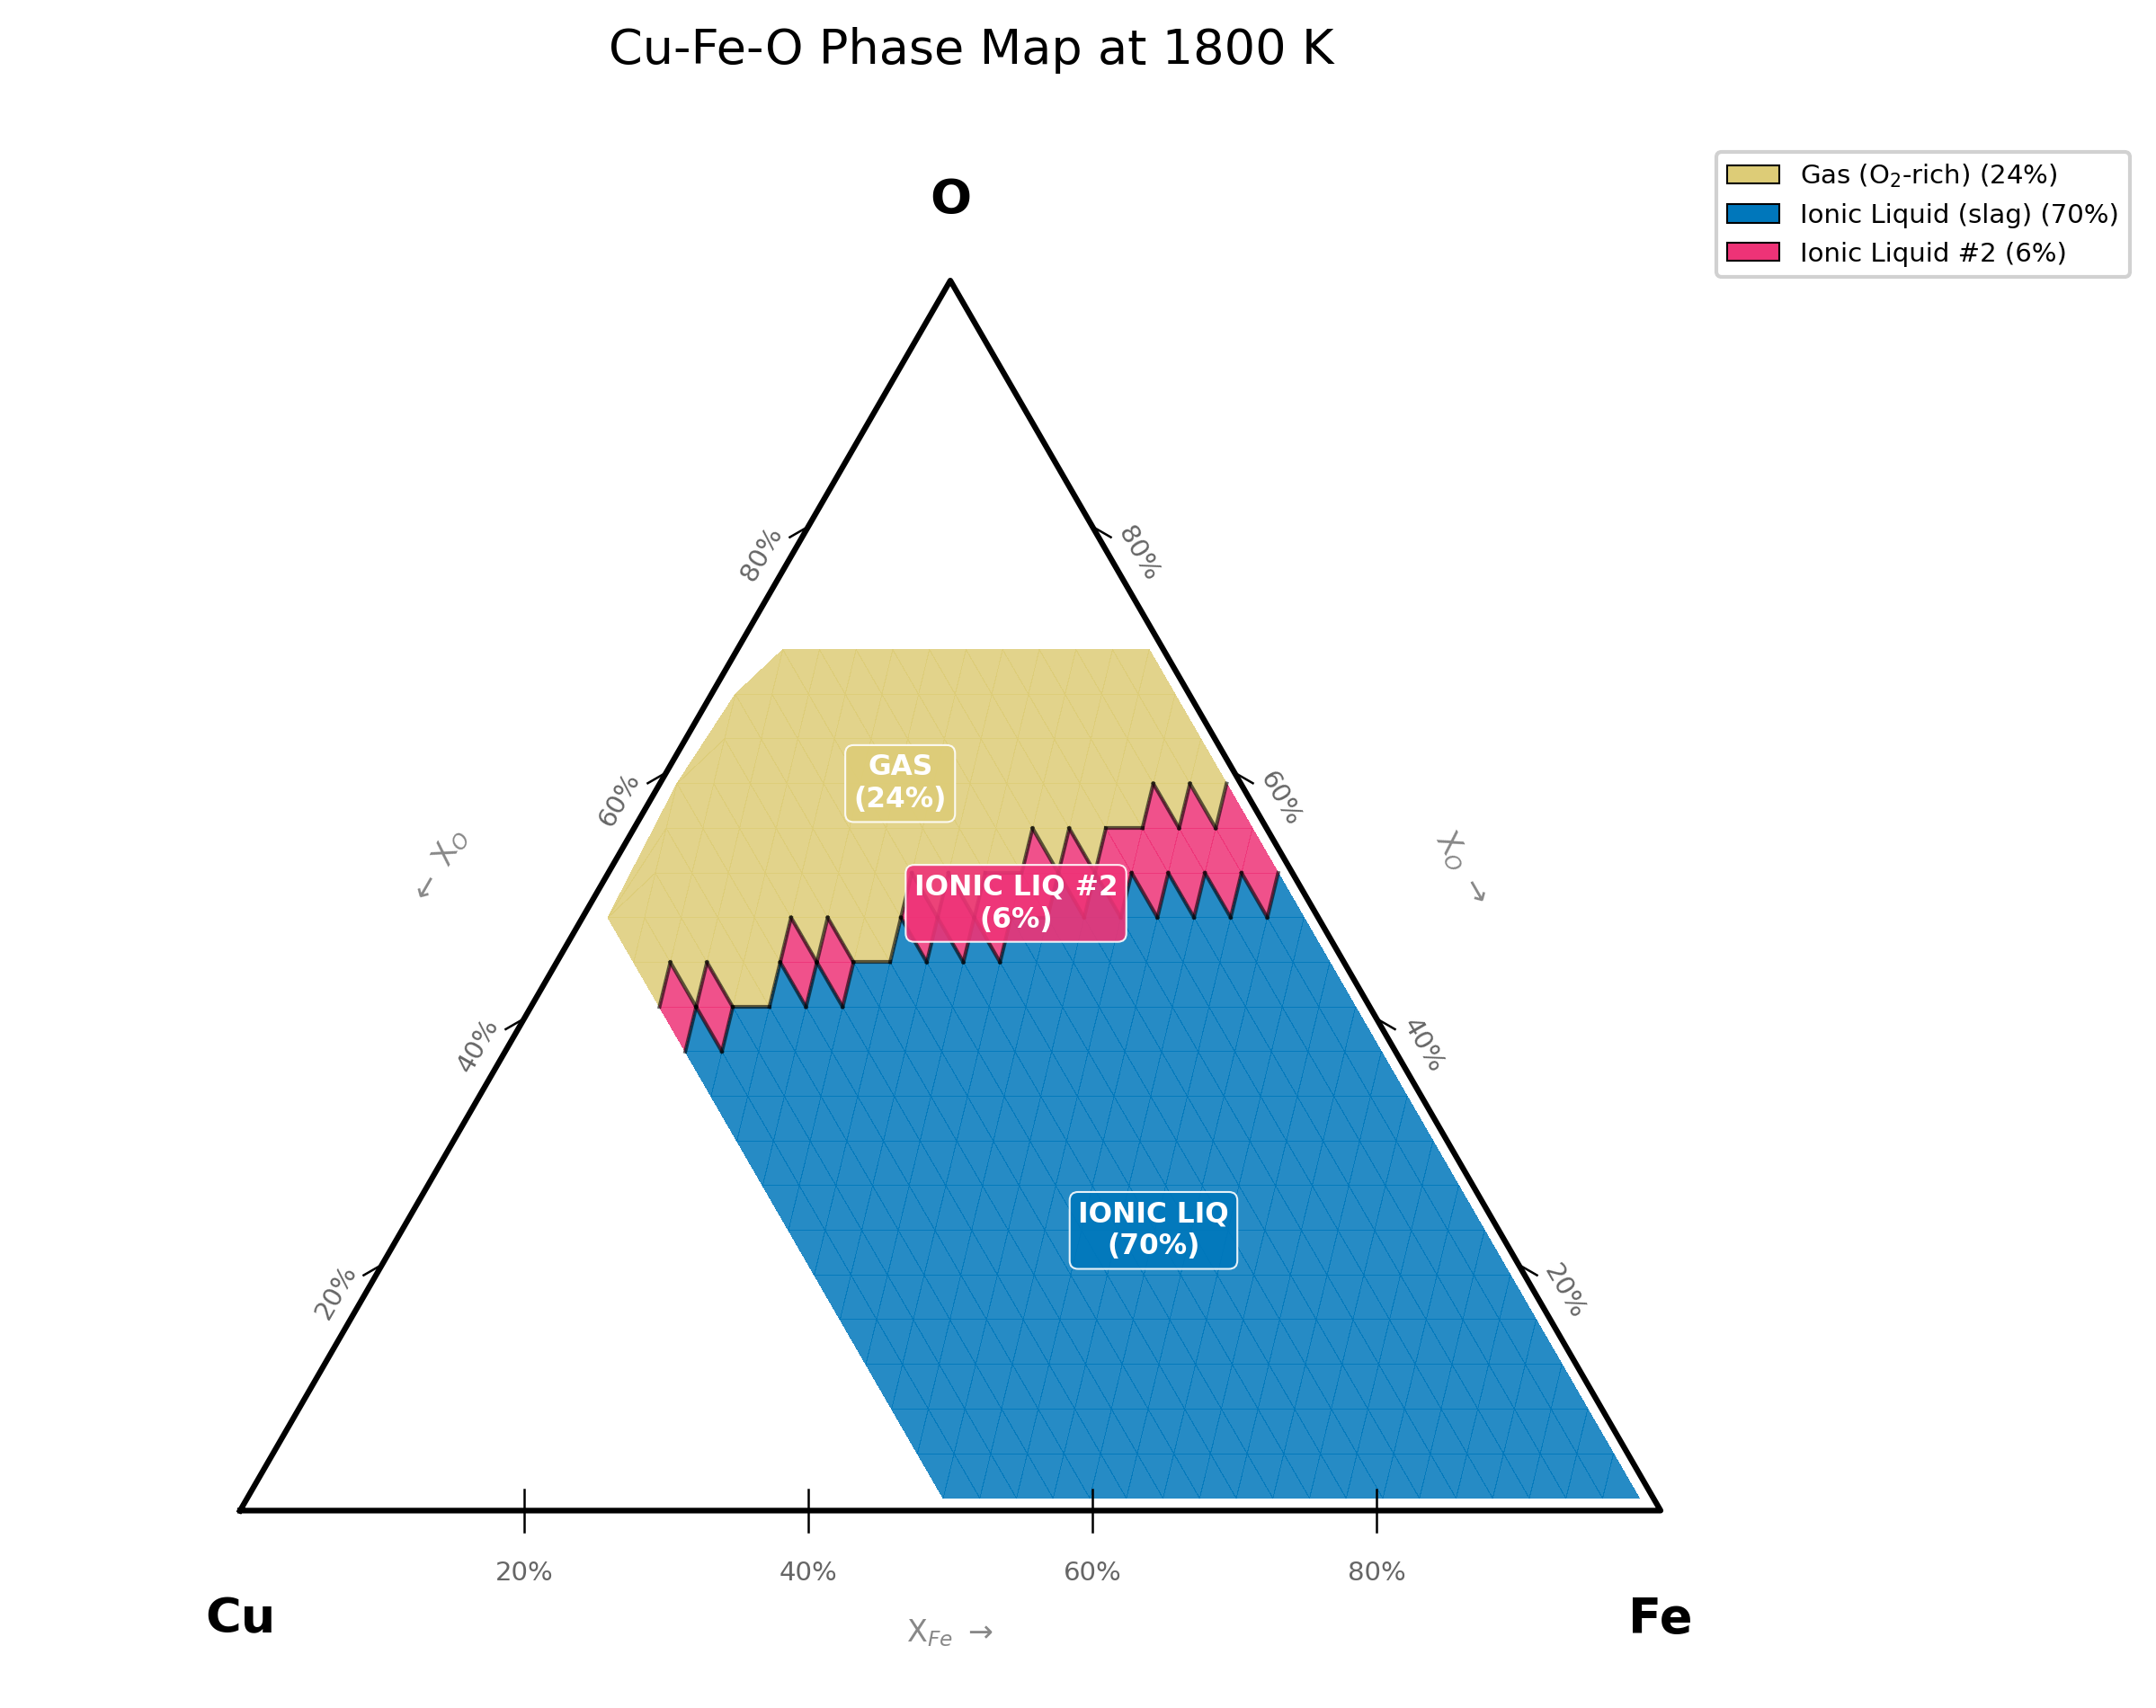
\includegraphics[width=0.75\textwidth]{phase_map_cu_fe_o_1800K.png}
    \caption{Phase map for Cu-Fe-O at \SI{1800}{\kelvin}. IONIC\_LIQ dominates ($\sim$70\% of points), confirming the system is fully liquid at steelmaking temperature. Script: \texttt{screening/plot\_ternary\_phase.py}.}
    \label{fig:phase_map_fe}
\end{figure}

\begin{figure}[H]
    \centering
    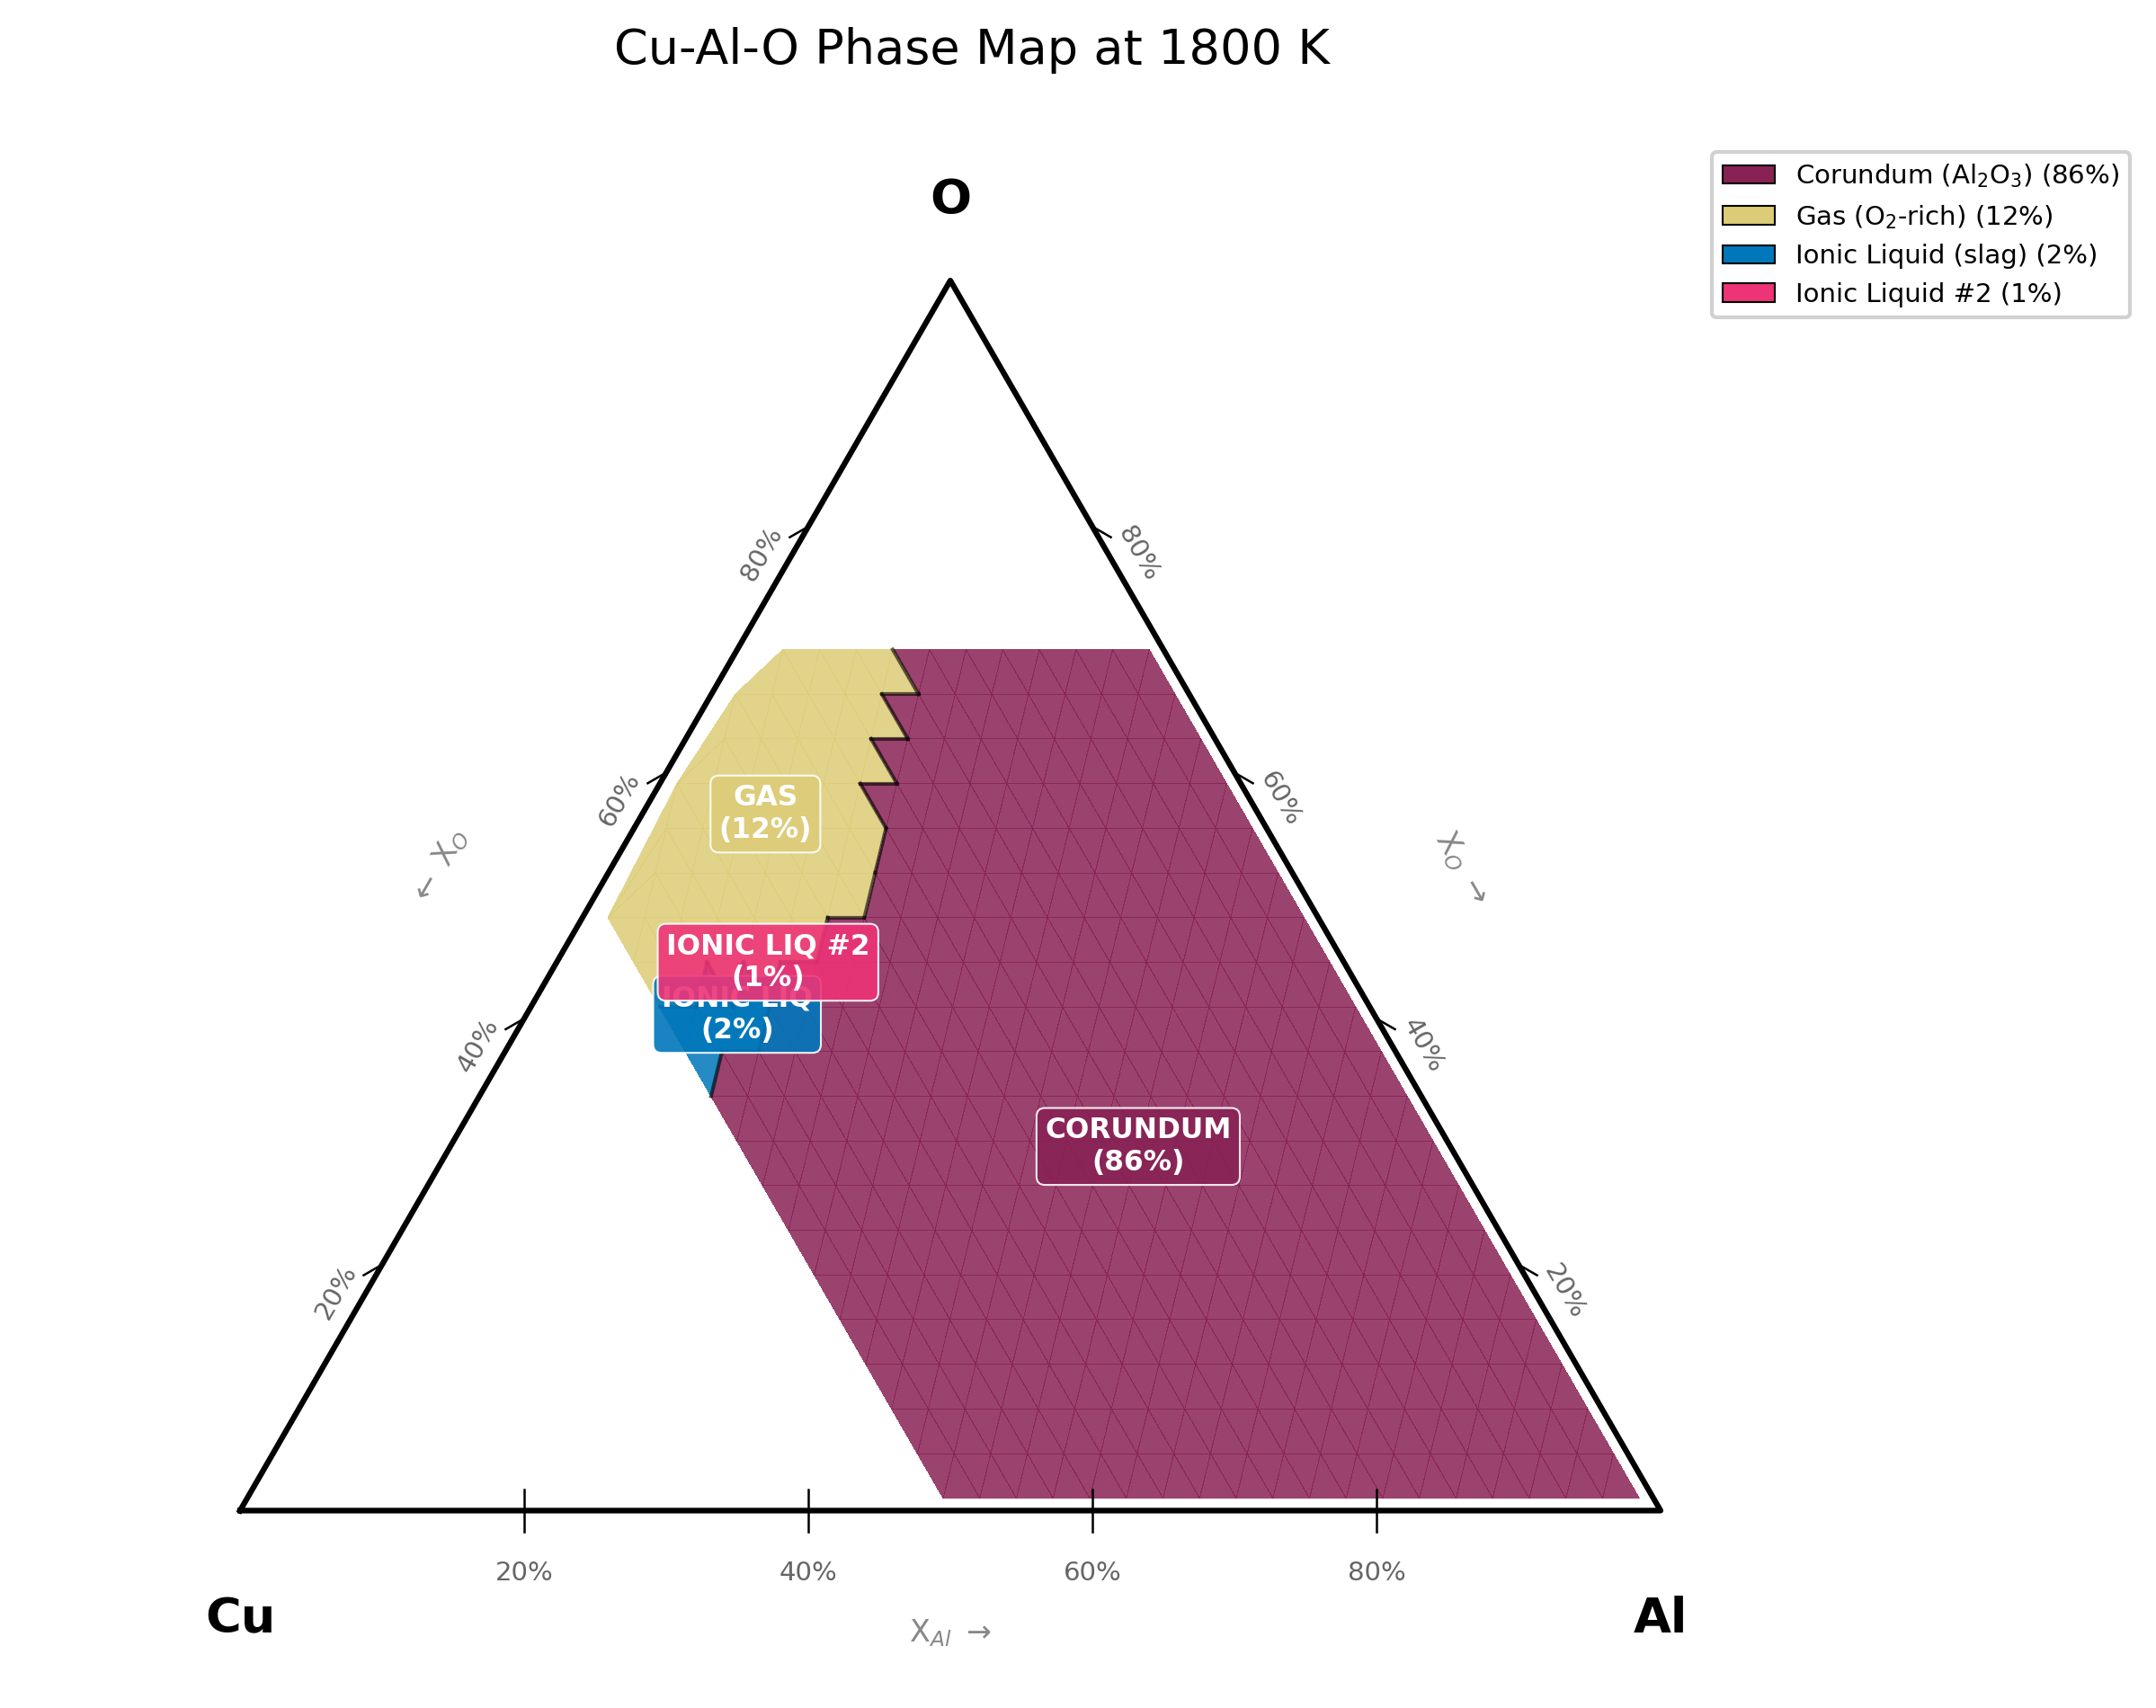
\includegraphics[width=0.75\textwidth]{phase_map_cu_al_o_1800K.png}
    \caption{Phase map for Cu-Al-O at \SI{1800}{\kelvin}. Large CORUNDUM (Al$_2$O$_3$) region persists ($\sim$86\% of points), reflecting Al$_2$O$_3$'s high melting point (\SI{2072}{\celsius}). Cu-rich corner is ionic liquid.}
    \label{fig:phase_map_al}
\end{figure}

\begin{figure}[H]
    \centering
    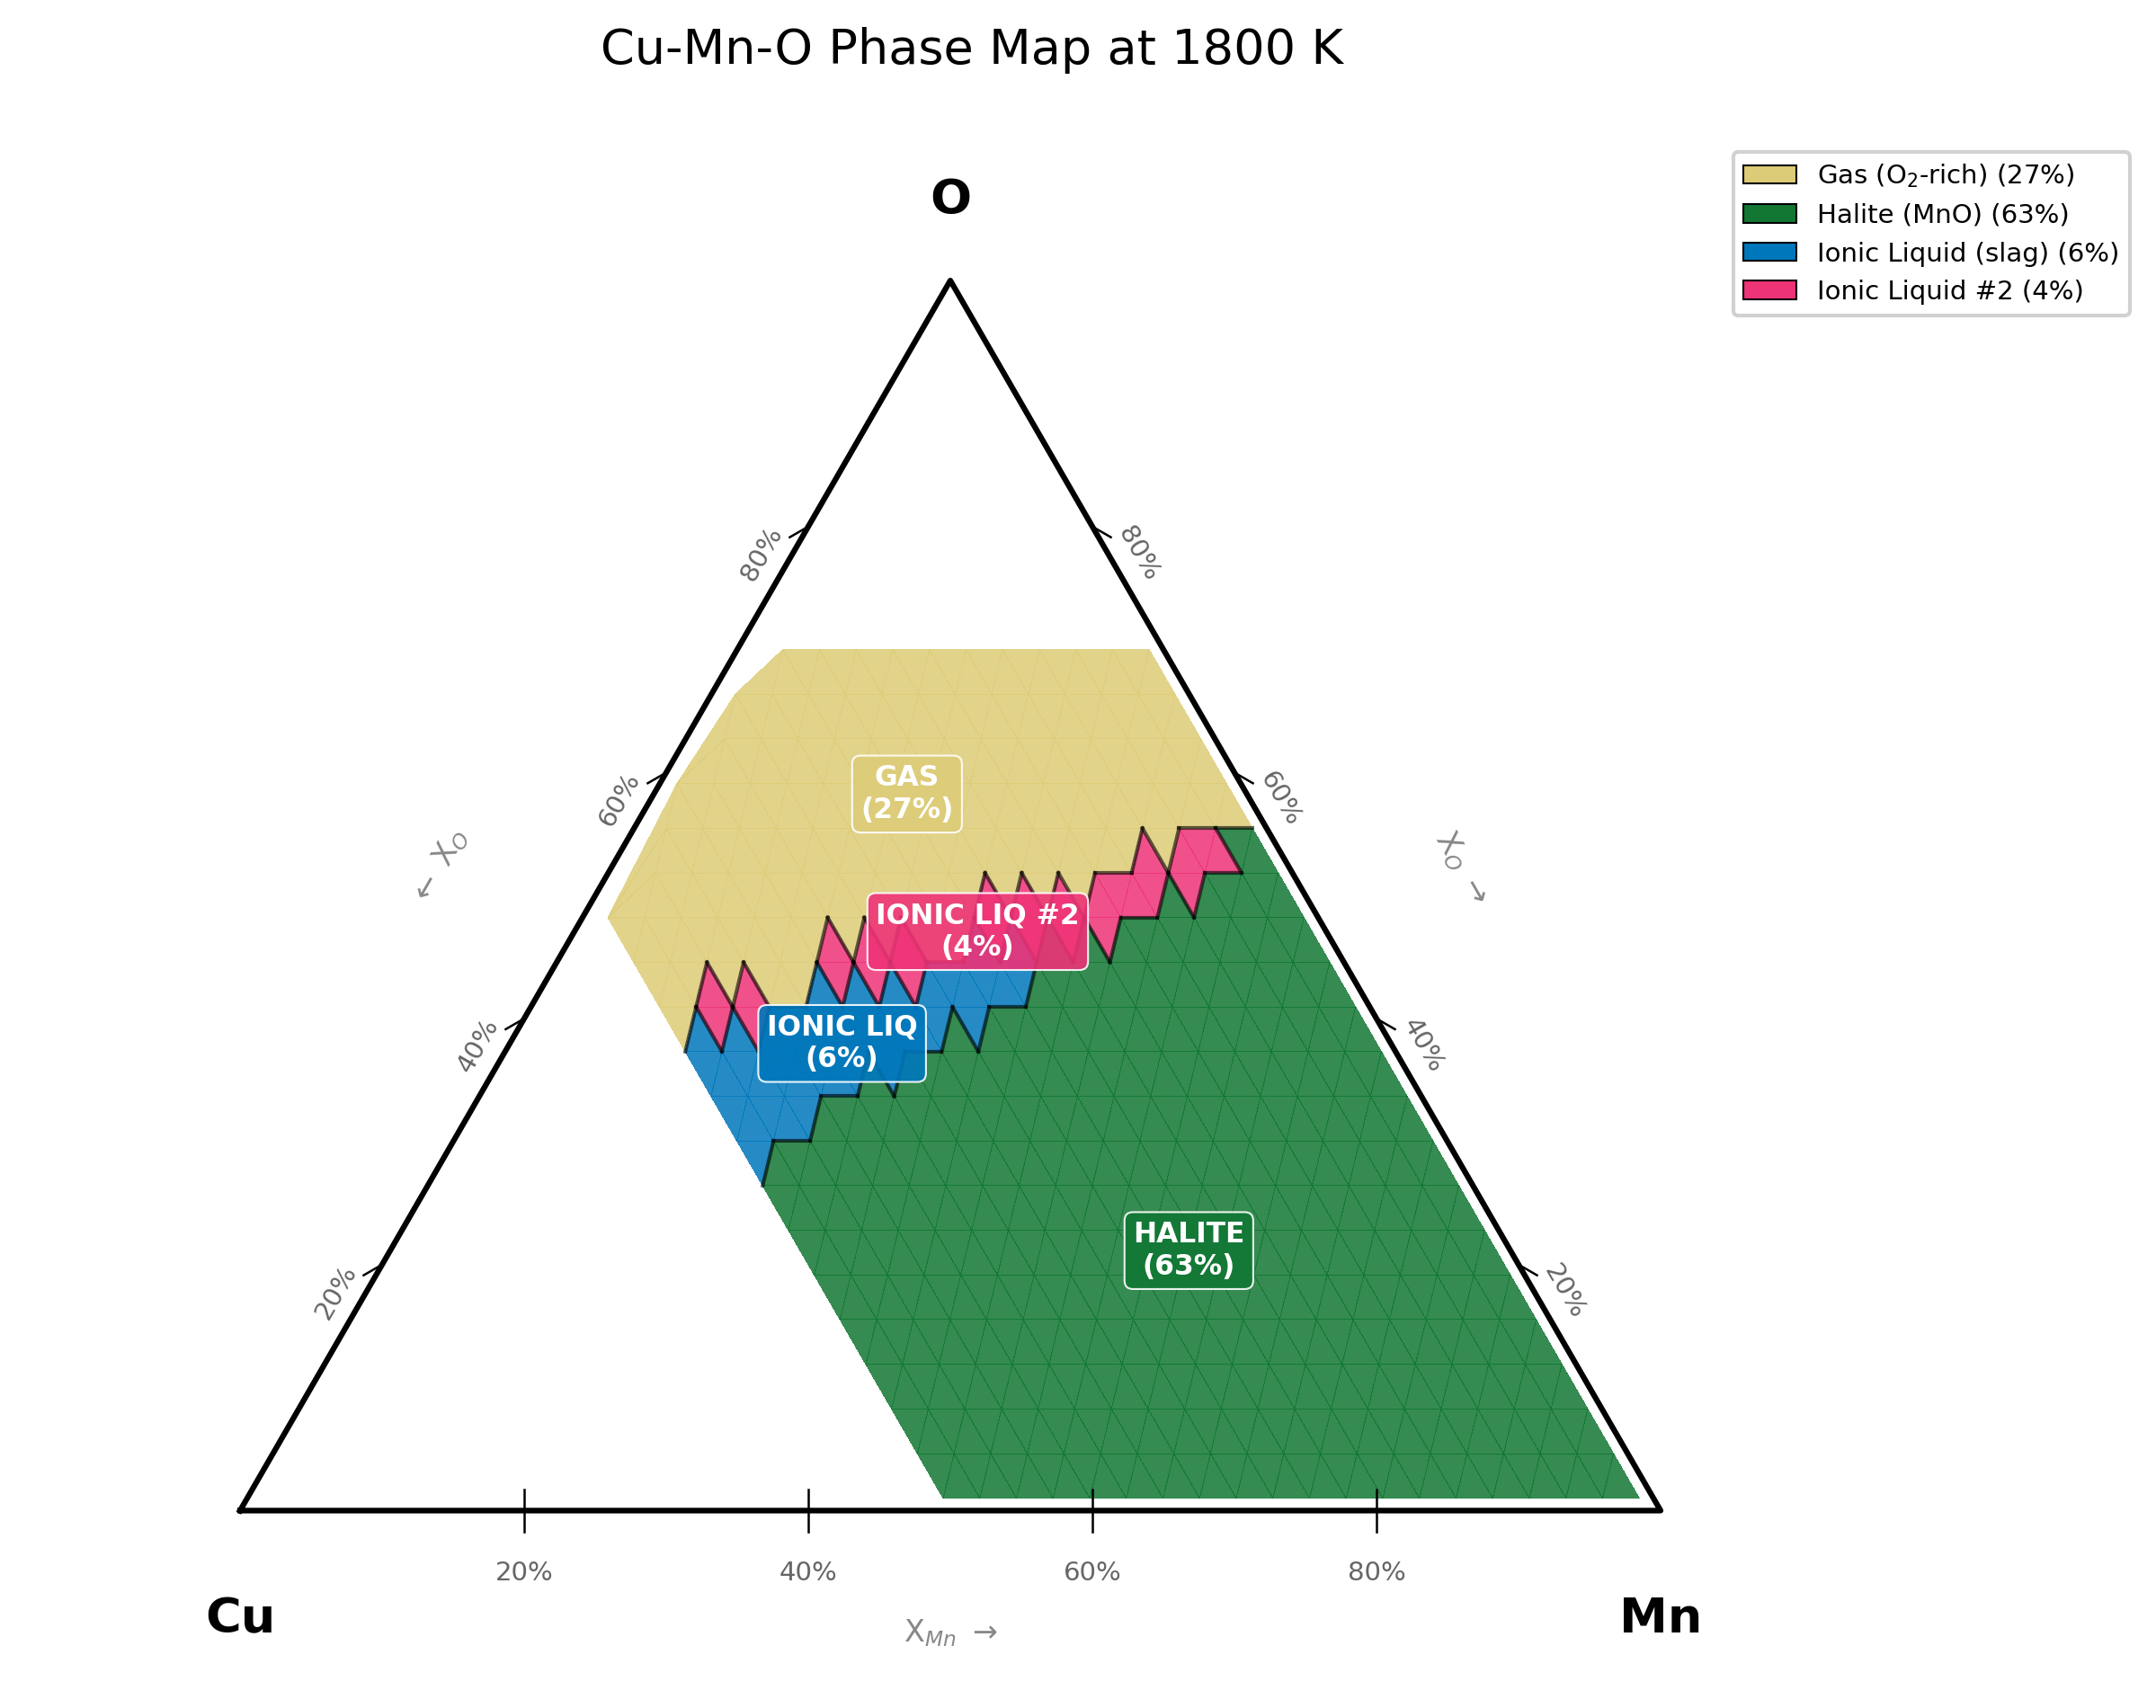
\includegraphics[width=0.75\textwidth]{phase_map_cu_mn_o_1800K.png}
    \caption{Phase map for Cu-Mn-O at \SI{1800}{\kelvin}. HALITE (MnO rock-salt) phase dominates ($\sim$63\%), with ionic liquid in the Cu-rich and O-rich corners.}
    \label{fig:phase_map_mn}
\end{figure}


%%%%%%%%%%%%%%%%%%%%%%%%%%%%%%%%%%%%%%%%%%%%%%%%%%%%%%%%%%%%%%%%%%%%%%%%%%%%%%%
% 8. DATABASE LANDSCAPE
%%%%%%%%%%%%%%%%%%%%%%%%%%%%%%%%%%%%%%%%%%%%%%%%%%%%%%%%%%%%%%%%%%%%%%%%%%%%%%%
\section{TC-Python Database Landscape}
\label{sec:databases}

\subsection{Thermodynamic Databases}

\begin{table}[H]
\caption{Thermodynamic Databases on the OSU VM}
\label{tab:thermo_dbs}
\centering
\renewcommand{\arraystretch}{1.2}
\begin{tabular}{|l|l|p{3in}|}
\hline
\rowcolor{headercolor}
\textcolor{white}{\textbf{Database}} & \textcolor{white}{\textbf{Status}} & \textcolor{white}{\textbf{Notes}} \\
\hline
TCOX14 & Available & Oxide systems. Our primary DB. Contains IONIC\_LIQ, SPINEL, CORUNDUM, etc. No metallic phases. \\
\hline
\rowcolor{altrow}
TCFE13 & Available & Steel systems. Contains FCC\_A1, BCC\_A2, LIQUID, CEMENTITE, etc. Limited oxide coverage. \\
\hline
TCFE12, TCFE11 & Available & Older steel databases. Same phase types as TCFE13. \\
\hline
\rowcolor{altrow}
SSUB3 & Available & Pure substance database. Fallback for elements not in TCOX14 (used for PbO, CeO$_2$). \\
\hline
\end{tabular}
\end{table}

\subsection{Mobility Databases (for DICTRA)}

\begin{table}[H]
\caption{Mobility Databases Tested on the OSU VM (March 14, 2026)}
\label{tab:mob_dbs}
\centering
\renewcommand{\arraystretch}{1.2}
\begin{tabular}{|l|c|p{3.2in}|}
\hline
\rowcolor{headercolor}
\textcolor{white}{\textbf{Database}} & \textcolor{white}{\textbf{Status}} & \textcolor{white}{\textbf{Notes}} \\
\hline
MOBFE8 & \textcolor{green!60!black}{Found} & Loads with TCFE13, TCFE12, TCFE11, \textbf{and TCOX14}. Primary steel mobility DB. \\
\hline
\rowcolor{altrow}
MOBFE7, 6, 5 & \textcolor{green!60!black}{Found} & Older versions. All load with all TCFE and TCOX14. \\
\hline
MOBFE9 & \textcolor{red}{Not found} & Not installed on this VM. \\
\hline
\rowcolor{altrow}
MOBOX1, MOBOX2 & \textcolor{red}{Not found} & Oxide mobility. Files may exist on disk but TC engine cannot load them (Error 1234). \\
\hline
MOBCU3, MOBCU2 & \textcolor{green!60!black}{Found} & Copper-specific mobility. SER reference state warning for O-containing systems. MOBCU2 fails with Cu-Fe-O on TCFE13. \\
\hline
\rowcolor{altrow}
MOBNI5, MOBNI4 & \textcolor{green!60!black}{Found} & Nickel mobility. Creates FCC\_L12 and BCC\_B2 ordered composition sets. \\
\hline
MOBAL3 & \textcolor{green!60!black}{Found} & Aluminum mobility. ``O INPUT IGNORED'' warning on O-containing systems but still loads. \\
\hline
\rowcolor{altrow}
MOBAL2 & Partial & Loads without O. Cu-Fe-O and Cu-Fe-Mn-O crash with calculation error. \\
\hline
\end{tabular}
\end{table}

\subsection{API Lessons}

\begin{enumerate}[leftmargin=*]
    \item \textbf{Empty element list is a false positive}: \texttt{select\_database\_and\_elements(db, [])} with an empty element list just checks if the database \textit{file} exists, not whether it can actually load. MOBOX1/MOBOX2 files exist on disk but the TC engine throws Error 1234 when trying to parse them. Always test with real elements.

    \item \textbf{Kinetic System API differs from thermodynamic}: The \texttt{System} object returned by \texttt{select\_thermodynamic\_and\_kinetic\_databases\_with\_elements()} does \textbf{not} have \texttt{get\_phase\_names()}. Instead, use \texttt{get\_phases\_in\_system()} and \texttt{get\_elements\_in\_system()}.

    \item \textbf{VM workflow}: Always download ZIP from GitHub, extract, and run. Never \texttt{git pull} on the VM (git may not be installed, and Citrix clipboard corrupts file transfers).
\end{enumerate}


%%%%%%%%%%%%%%%%%%%%%%%%%%%%%%%%%%%%%%%%%%%%%%%%%%%%%%%%%%%%%%%%%%%%%%%%%%%%%%%
% 9. DICTRA AND DIFFUSION KINETICS
%%%%%%%%%%%%%%%%%%%%%%%%%%%%%%%%%%%%%%%%%%%%%%%%%%%%%%%%%%%%%%%%%%%%%%%%%%%%%%%
\section{DICTRA and Diffusion Kinetics}
\label{sec:dictra}

\subsection{What DICTRA Does}

DICTRA (DIffusion Controlled TRAnsformations) solves the multicomponent diffusion equation:
\begin{equation}
    \frac{\partial c_i}{\partial t} = \nabla \cdot \left( \sum_j D_{ij} \nabla c_j \right)
    \label{eq:diffusion}
\end{equation}
where $D_{ij}$ is the interdiffusion coefficient matrix, computed from mobility data at each time step using local thermodynamic equilibrium (the ``DICTRA assumption'').

In TC-Python, DICTRA is accessed via:
\begin{lstlisting}
system = session.select_thermodynamic_and_kinetic_databases_with_elements(
    "TCFE13", "MOBFE8", ["CU", "FE"]).get_system()
diff_calc = system.with_isothermal_diffusion_calculation()
\end{lstlisting}

\subsection{Why It Matters for Cu Removal}

Thermodynamics tells us \textit{whether} Cu capture is favorable. DICTRA~\cite{Andersson2002} tells us \textit{how fast}:
\begin{itemize}[leftmargin=*]
    \item How quickly does Cu diffuse from bulk steel to the steel/slag interface?
    \item How long must the slag contact the melt to achieve meaningful Cu removal?
    \item Does the geometry matter (flat interface vs.\ spherical oxide particles)?
\end{itemize}

If Cu diffusion in liquid Fe is fast (D $\sim 10^{-9}$ m$^2$/s at \SI{1800}{\kelvin}~\cite{Hino2010}), then a 10-minute furnace hold might remove Cu from a 1-cm-thick steel layer. If it is slow, we might need stirring, smaller particles, or longer treatment times.

\subsection{TC-Python Diffusion API}

The API provides:
\begin{itemize}[leftmargin=*]
    \item \textbf{Region}: A 1D spatial domain with width, grid, and initial composition profile
    \item \textbf{CalculatedGrid}: Linear, geometric, or double-geometric point distributions
    \item \textbf{ElementProfile}: Constant, linear, or step initial composition within a region
    \item \textbf{BoundaryCondition}: Closed system, fixed composition, or activity-based flux
    \item \textbf{Geometry}: Planar, cylindrical, or spherical
    \item \textbf{Solver}: Automatic, Classic, or Homogenization
\end{itemize}

The activity-based boundary condition is particularly relevant: it allows us to impose $a_{\text{Cu}} = 0.0006$ (the equilibrium value from TCOX14) at the steel surface, simulating the chemical potential drop that an oxide slag imposes. This avoids needing to model the slag phase explicitly.

\subsection{DICTRA Capability Test Results (March 14, 2026)}

A 6-phase DICTRA test script ran on the OSU VM ($\sim$1 hour runtime). Results split into two categories: API discovery (Phases 1--2, succeeded) and actual diffusion calculations (Phases 3--6, failed due to fixable script bugs).

\subsubsection{Phase 1--2: Database Compatibility \& API Discovery}

Of 312 thermo $\times$ mobility combinations tested, \textbf{232 loaded successfully} and \textbf{40 unique pairs} support isothermal diffusion calculations. Key findings:

\begin{itemize}[leftmargin=*]
    \item MOBFE8/7/6/5 all load with TCFE13/12/11 and TCOX14
    \item MOBFE9, MOBOX1, MOBOX2: \textbf{not found} on this VM
    \item MOBCU3 loads for all element sets (copper-specific mobility)
    \item The kinetic System object has 20 public methods; the correct phase enumeration method is \texttt{get\_phases\_in\_system()} (not \texttt{get\_phase\_names()} or \texttt{get\_phases()})
    \item \texttt{PhaseComposition} class is \textbf{not available} in the \texttt{tc\_python} namespace
    \item All three DICTRA geometries confirmed: planar, cylindrical, spherical
    \item All required API classes confirmed: \texttt{Region}, \texttt{CalculatedGrid}, \texttt{CompositionProfile}, \texttt{ElementProfile}, \texttt{BoundaryCondition}, \texttt{Unit}, all 3 solvers, \texttt{SimulationTime}
\end{itemize}

\subsubsection{Phase 3--6: Initial Failures and Script Bug Fixes}

The initial run (March 14 AM) failed in Phases 3--6 due to three script bugs: wrong phase enumeration methods, empty phases list preventing pair selection, and an undefined \texttt{calc\_succeeded} variable. All three were fixed, and LIQUID phase support at \SI{1800}{\kelvin} was added.

\subsubsection{Re-Run Results (March 14 PM: Fixed Script)}

After fixing the script bugs, Phases 1--2 reproduced identically. Phase 3 reached the actual diffusion calculation but failed with a \textbf{new error}: the \texttt{Region} object does not specify which thermodynamic phase is the diffusion matrix.

Three API patterns were attempted:
\begin{enumerate}[leftmargin=*]
    \item \textbf{Pattern A} (CompositionProfile + ElementProfile): \texttt{IndexOutOfBoundsException: Index 0 out of bounds for length 0}. The DICTRA engine's internal phase list is empty because no phase was assigned to the Region.
    \item \textbf{Pattern B} (PhaseComposition API): \texttt{'Region' object has no attribute 'add\_phase\_composition'}. This method does not exist in the installed TC-Python version.
    \item \textbf{Pattern C} (minimal region): \texttt{All regions must have one or more phases}. TC-Python's own validation confirms the missing phase specification.
\end{enumerate}

Phases 4--6 were skipped because Phase 3 failed. A subsequent run probed \texttt{dir(Region(...))} and discovered 8 methods, including the solution: \texttt{Region.add\_phase(phase\_name)}. With this call added, Phase 3 succeeded: Cu diffusion in FCC\_A1 at 1200\,K for 3600\,s returned a 50-point composition profile (0.0000--0.5000\,wt\% Cu). The script was updated to add \texttt{.add\_phase()} to all Phases 4--6, with temperature-dependent phase selection (LIQUID above 1700\,K, FCC\_A1 below).

\subsubsection{Run 3 Results: Phases 4--6 (March 14, 6:42 PM)}

With the \texttt{.add\_phase()} fix applied to all phases, the full 6-phase test completed in $\sim$30 minutes. Phases 1--3 reproduced prior results. Phases 4--6 produced new data:

\paragraph{Phase 4: Cu Diffusion Coefficients vs Temperature.}
The script ran short (1\,s) diffusion simulations at 8 temperatures and estimated $D_{\text{Cu}}$ from profile displacement:

\begin{center}
\begin{tabular}{l c r}
\hline
\rowcolor{headercolor}
\textcolor{white}{\textbf{Temperature}} & \textcolor{white}{\textbf{Phase}} & \textcolor{white}{\textbf{$D_{\text{Cu}}$ (m$^2$/s)}} \\
\hline
1073--1673\,K & FCC\_A1 & $<10^{-15}$ (below grid resolution) \\
\rowcolor{altrow}
1773\,K & LIQUID & $9.63 \times 10^{-10}$ \\
1800\,K & LIQUID & $9.63 \times 10^{-10}$ \\
\rowcolor{altrow}
1873\,K & LIQUID & $9.63 \times 10^{-10}$ \\
\hline
\end{tabular}
\end{center}

The liquid-phase value $D_{\text{Cu}} \approx 10^{-9}$\,m$^2$/s independently confirms the literature value \cite{Hino2010}. The solid-state values appear as zero because 1\,s simulation time is too short to resolve FCC diffusion ($D \sim 10^{-15}$\,m$^2$/s at 1073\,K gives $\sqrt{2Dt} \approx 45$\,nm, well below the 100\,$\mu$m grid spacing).

\paragraph{Phase 5: Two-Region Steel/Slag Interface.}
Two tests modeled Cu transport across a metal/oxide boundary using TCOX14 + MOBFE8 (Cu-Fe-O):

\begin{itemize}[leftmargin=*]
    \item \textbf{Test A} (two LIQUID regions): \textbf{Failed.} The \texttt{CompositionProfile} only specified Cu; DICTRA requires all non-dependent elements (Cu, Fe with O as dependent). This is a script bug, not an API limitation.
    \item \textbf{Test B} (FCC\_A1 $|$ IONIC\_LIQ\#2 at 1800\,K): \textbf{Succeeded.} Steel (0.3\% Cu) and oxide slag ran as a diffusion couple for 3600\,s. Cu redistributed: 36.2\,wt\% in the steel-side phase, 57.0\,wt\% in the slag-side phase. These are phase-internal compositions (not bulk averages), confirming DICTRA handles Cu partitioning across a metal/slag interface.
\end{itemize}

\paragraph{Phase 6: Boundary Conditions and Geometries.}
All four tests succeeded using TCFE13 + MOBFE8 (Cu-Fe) with FCC\_A1 at 1200\,K:

\begin{itemize}[leftmargin=*]
    \item \textbf{Fixed composition BC}: Cu = 0.50\,wt\% at left wall, 0.10\,wt\% at right wall after 3600\,s. Gradient as expected.
    \item \textbf{Activity BC} ($a_{\text{Cu}} = 0.001$ at right wall): Cu remained at 0.30\,wt\% everywhere. The imposed activity already matches equilibrium at this composition, so no driving force exists; the simulation is self-consistent but not Cu-removing.
    \item \textbf{Cylindrical geometry}: 50\,$\mu$m radius, 600\,s. Cu diffused inward from the surface.
    \item \textbf{Spherical geometry}: 50\,$\mu$m radius sphere. Cu at center = 0.04\,wt\%, surface = 0.30\,wt\%, showing radial depletion toward the core.
\end{itemize}

\subsubsection{Implications}

Five of six DICTRA capability tests now succeed. The confirmed capabilities directly map to the Honda project needs:

\begin{itemize}[leftmargin=*]
    \item \textbf{Cu diffusion in liquid steel}: $D_{\text{Cu}} = 9.63 \times 10^{-10}$\,m$^2$/s at 1800\,K (matches literature)
    \item \textbf{Steel/slag interface}: two-region modeling with FCC\_A1 and IONIC\_LIQ works; Cu partitions across the boundary
    \item \textbf{Activity-based BC}: can impose $a_{\text{Cu}}$ from oxide equilibrium at the steel surface
    \item \textbf{Spherical geometry}: can model Cu diffusion into oxide particles (relevant to powder-injection experiments)
\end{itemize}

The one remaining failure (Phase 5 Test A) is a script bug: the composition profile must specify all non-dependent elements, not just Cu. The DICTRA API itself is fully functional for all planned calculations.


%%%%%%%%%%%%%%%%%%%%%%%%%%%%%%%%%%%%%%%%%%%%%%%%%%%%%%%%%%%%%%%%%%%%%%%%%%%%%%%
% 10. CuFe2O4 DECOMPOSITION
%%%%%%%%%%%%%%%%%%%%%%%%%%%%%%%%%%%%%%%%%%%%%%%%%%%%%%%%%%%%%%%%%%%%%%%%%%%%%%%
\section{CuFe$_2$O$_4$: Decomposing the Driving Force}

CuFe$_2$O$_4$ has the strongest $\Delta G$ ($-112$ kJ at \SI{1800}{\kelvin}), but its reaction involves both Cu capture \textit{and} Fe$^{2+} \to$ Fe$^{3+}$ oxidation. How much of the driving force comes from Cu affinity alone?

\subsection{Method}

We computed an alternative reaction using Fe$_2$O$_3$ instead of FeO:
\[
    \text{Cu} + \text{Fe}_2\text{O}_3 + \tfrac{1}{2}\text{O}_2 \to \text{CuFe}_2\text{O}_4
\]

In this reaction, Fe is \textit{already} at the $+3$ state, so any $\Delta G$ is purely from Cu incorporation into the spinel.

\subsection{Result}

\begin{itemize}[leftmargin=*]
    \item Cu-capture component: $-45.7$ kJ/mol (41\% of total)
    \item Fe-oxidation component: $-66.2$ kJ/mol (59\% of total)
    \item \textbf{Cu-capture alone is independently favorable}
\end{itemize}

Even without the Fe oxidation bonus, Cu incorporation into the spinel is thermodynamically driven. After activity correction ($n_{\text{Cu}} = 1$, penalty $= +54.9$ kJ), the Cu-capture component becomes $-45.7 + 54.9 = +9.2$ kJ, which is marginal. But the full reaction still sits at $-57.0$ kJ because the Fe oxidation energy is ``free'' (Fe is already being oxidized in the steelmaking slag).


%%%%%%%%%%%%%%%%%%%%%%%%%%%%%%%%%%%%%%%%%%%%%%%%%%%%%%%%%%%%%%%%%%%%%%%%%%%%%%%
% 11. V2O5: A COMPLICATED CASE
%%%%%%%%%%%%%%%%%%%%%%%%%%%%%%%%%%%%%%%%%%%%%%%%%%%%%%%%%%%%%%%%%%%%%%%%%%%%%%%
\section{V$_2$O$_5$: Two Products, Two Stories}

V$_2$O$_5$ can form two different Cu compounds:

\begin{enumerate}[leftmargin=*]
    \item \textbf{Cu$_3$V$_2$O$_8$} ($n_{\text{Cu}} = 3$): Pure $\Delta G = -109$ kJ, but activity-corrected $\Delta G_{\text{eff}} = +55.6$ kJ. \textbf{Unfavorable} under steelmaking dilution.

    \item \textbf{CuV$_2$O$_6$} ($n_{\text{Cu}} = 1$): Pure $\Delta G = -45$ kJ, activity-corrected $\Delta G_{\text{eff}} = +9.9$ kJ. \textbf{Uncertain}: near zero, within $\gamma_{\text{Cu}}$ sensitivity range.
\end{enumerate}

Our initial analysis only considered Cu$_3$V$_2$O$_8$ (ranked \#2 by pure $\Delta G$) and concluded V$_2$O$_5$ ``fails.'' This was premature; the single-Cu product CuV$_2$O$_6$ is much more favorable under dilute conditions.

\begin{insight}[Lesson: Check All Stoichiometries]
Under dilute-Cu conditions, multi-Cu products are heavily penalized. Always check whether the parent oxide can form a 1:1 Cu product. The ``top 6 by pure $\Delta G$'' filter misses CuV$_2$O$_6$ because the 3-Cu product ranked higher. Selection criteria must account for the conditions under which the reaction will actually occur.
\end{insight}

Bureau of Mines researchers tested V$_2$O$_5$ via oxide injection into molten steel and found it more effective than Al$_2$O$_3$ and MnO$_2$, but results remained far below commercially viable levels; slag Cu concentrations would need to increase 20--80$\times$ for economic feasibility \cite{911metallurgist}. At higher Cu concentrations and lower temperatures, both V$_2$O$_5$ products could become thermodynamically favorable.


%%%%%%%%%%%%%%%%%%%%%%%%%%%%%%%%%%%%%%%%%%%%%%%%%%%%%%%%%%%%%%%%%%%%%%%%%%%%%%%
% 12. EXPERIMENTAL OUTLOOK
%%%%%%%%%%%%%%%%%%%%%%%%%%%%%%%%%%%%%%%%%%%%%%%%%%%%%%%%%%%%%%%%%%%%%%%%%%%%%%%
\section{Toward Experimental Validation}

\subsection{Recommended Candidates}

Based on the activity-corrected analysis:

\begin{enumerate}[leftmargin=*]
    \item \textbf{FeO/Fe$_2$O$_3$} (forming CuFe$_2$O$_4$ spinel): $\Delta G_{\text{eff}} = -57$ kJ. Robust across all $\gamma_{\text{Cu}}$ values. Already present in steelmaking slag. \textbf{Top pick.}

    \item \textbf{MnO} (forming CuMn$_2$O$_4$ spinel): $\Delta G_{\text{eff}} = -9.5$ kJ. Marginal but favorable. Also present in steelmaking slag. Slag basicity (MnO:SiO$_2$ ratio) can be tuned.

    \item \textbf{V$_2$O$_5$} (forming CuV$_2$O$_6$): $\Delta G_{\text{eff}} = +10$ kJ (uncertain). Bureau of Mines tested V$_2$O$_5$ injection (more effective than Al$_2$O$_3$/MnO$_2$ but still far below viable~\cite{911metallurgist}). Worth testing at higher Cu levels where activity penalty is smaller.
\end{enumerate}

\subsection{Mass Balance Estimates}

A local calculator (\texttt{mass\_balance\_calculator.py}) computes stoichiometric oxide requirements for each candidate. For a \SI{0.5}{\kilogram} steel melt going from 0.30 to 0.10\,wt\% Cu (\SI{1.0}{\gram} Cu to remove):

\begin{table}[H]
\caption{Oxide Requirements for 0.5\,kg Steel, 0.3\% $\to$ 0.1\% Cu}
\label{tab:mass_balance}
\centering
\renewcommand{\arraystretch}{1.15}
\footnotesize
\begin{tabular}{|l|l|r|r|r|}
\hline
\rowcolor{headercolor}
\textcolor{white}{\textbf{Oxide}} & \textcolor{white}{\textbf{Product}} & \textcolor{white}{\textbf{Stoich (g)}} & \textcolor{white}{\textbf{3$\times$ (g)}} & \textcolor{white}{\textbf{wt\%}} \\
\hline
Fe$_2$O$_3$ & CuFe$_2$O$_4$ & 2.51 & 7.54 & 1.51 \\
\hline
\rowcolor{altrow}
V$_2$O$_5$ & Cu$_3$V$_2$O$_8$ & 0.95 & 2.86 & 0.57 \\
\hline
MnO & CuMn$_2$O$_4$ & 2.23 & 6.70 & 1.34 \\
\hline
\rowcolor{altrow}
SiO$_2$ & Cu$_2$SiO$_4$ & 0.47 & 1.42 & 0.28 \\
\hline
Al$_2$O$_3$ & CuAl$_2$O$_4$ & 1.60 & 4.81 & 0.96 \\
\hline
\end{tabular}
\end{table}

All oxide doses are small ($<$2\,wt\% at 3$\times$ excess), confirming that material cost is not a constraint. V$_2$O$_5$ is the most efficient per gram (3 Cu captured per mol oxide), but Fe$_2$O$_3$ has the strongest thermodynamic driving force.

\begin{insight}[Diffusion is Not the Bottleneck]
$D_{\text{Cu}} = 9.63 \times 10^{-10}$\,m$^2$/s in liquid Fe at \SI{1800}{\kelvin} (from DICTRA Phase~4). For a \SI{100}{\micro\meter} particle, the diffusion time is $r^2/2D \approx$~\SI{5}{\second}. Cu reaches any particle within seconds. The rate-limiting step will be the chemical reaction at the particle surface, not transport through the melt.
\end{insight}

\textbf{Particle size trade-off:} Smaller particles ($R = 10$--\SI{50}{\micro\meter}) give orders of magnitude more surface area per gram but dissolve faster into slag. At $R = \SI{100}{\micro\meter}$, \SI{7.5}{\gram} of Fe$_2$O$_3$ provides $3.4 \times 10^5$ particles with \SI{432}{\centi\meter\squared} total surface area.

\subsection{Cu Removal Rate Prediction (DICTRA)}

A spherical particle model (\texttt{cu\_removal\_rate.py}) simulates the Cu depletion shell around an oxide particle in liquid steel. The setup:

\begin{itemize}[leftmargin=*]
    \item Spherical geometry: \SI{5}{\milli\meter} steel shell around particle (center = particle surface)
    \item Left BC: fixed composition, Cu = 0.01\,wt\% at particle surface (oxide equilibrium sink)
    \item Right BC: closed system (far-field bulk steel at 0.30\,wt\% Cu)
    \item Sweep: 5 particle radii (25--\SI{500}{\micro\meter}) $\times$ 4 contact times (1--30\,min)
    \item Database: TCFE13 + MOBFE8, LIQUID phase at \SI{1800}{\kelvin}
\end{itemize}

\textbf{Results (20/20 calculations succeeded):} Each particle creates a Cu-depleted zone extending $\sim$250--\SI{500}{\micro\meter} into the surrounding steel. Cu captured per particle ranges from $2.2 \times 10^{-3}$\,mg (25\,$\mu$m, 1\,min) to $8.9 \times 10^{-2}$\,mg (500\,$\mu$m, 30\,min). Larger particles capture more per particle, but smaller particles provide orders of magnitude more surface area per gram of oxide.

\begin{figure}[H]
    \centering
    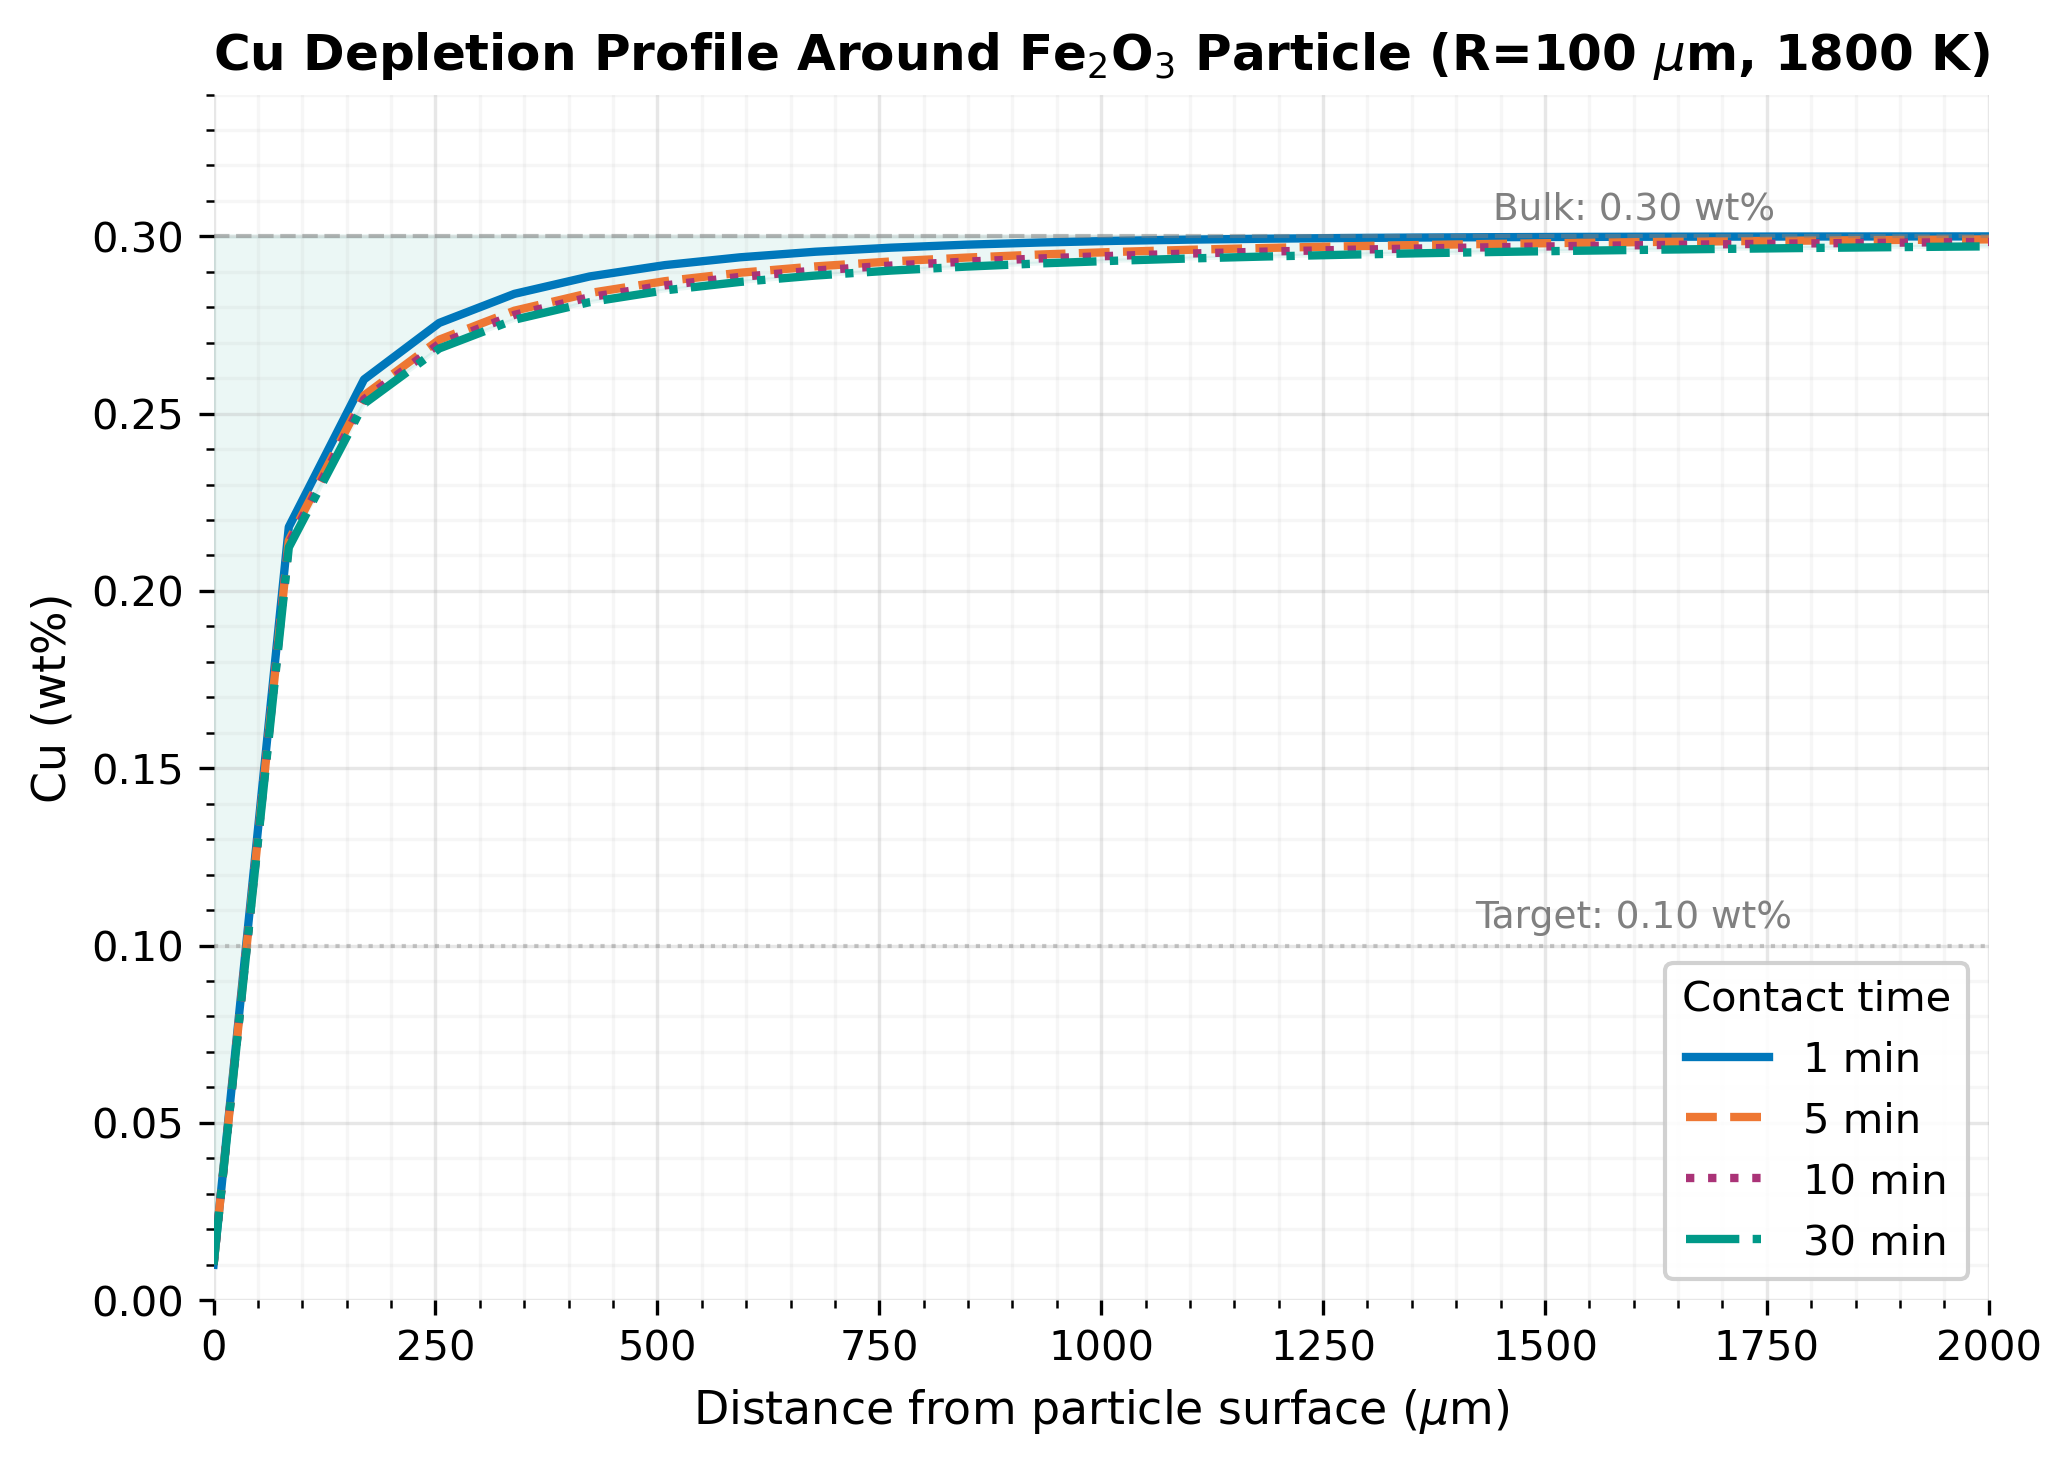
\includegraphics[width=0.75\textwidth]{cu_removal_profiles.png}
    \caption{Cu depletion profile around a \SI{100}{\micro\meter} Fe$_2$O$_3$ particle in liquid steel at \SI{1800}{\kelvin}. The oxide surface (left) maintains Cu $\approx$ 0.01\,wt\%, creating a concentration gradient that draws Cu from the bulk (0.30\,wt\%). Longer contact times widen the depleted zone. Generated by \texttt{plot\_cu\_removal\_rate.py}.}
    \label{fig:cu_removal_profiles}
\end{figure}

\begin{figure}[H]
    \centering
    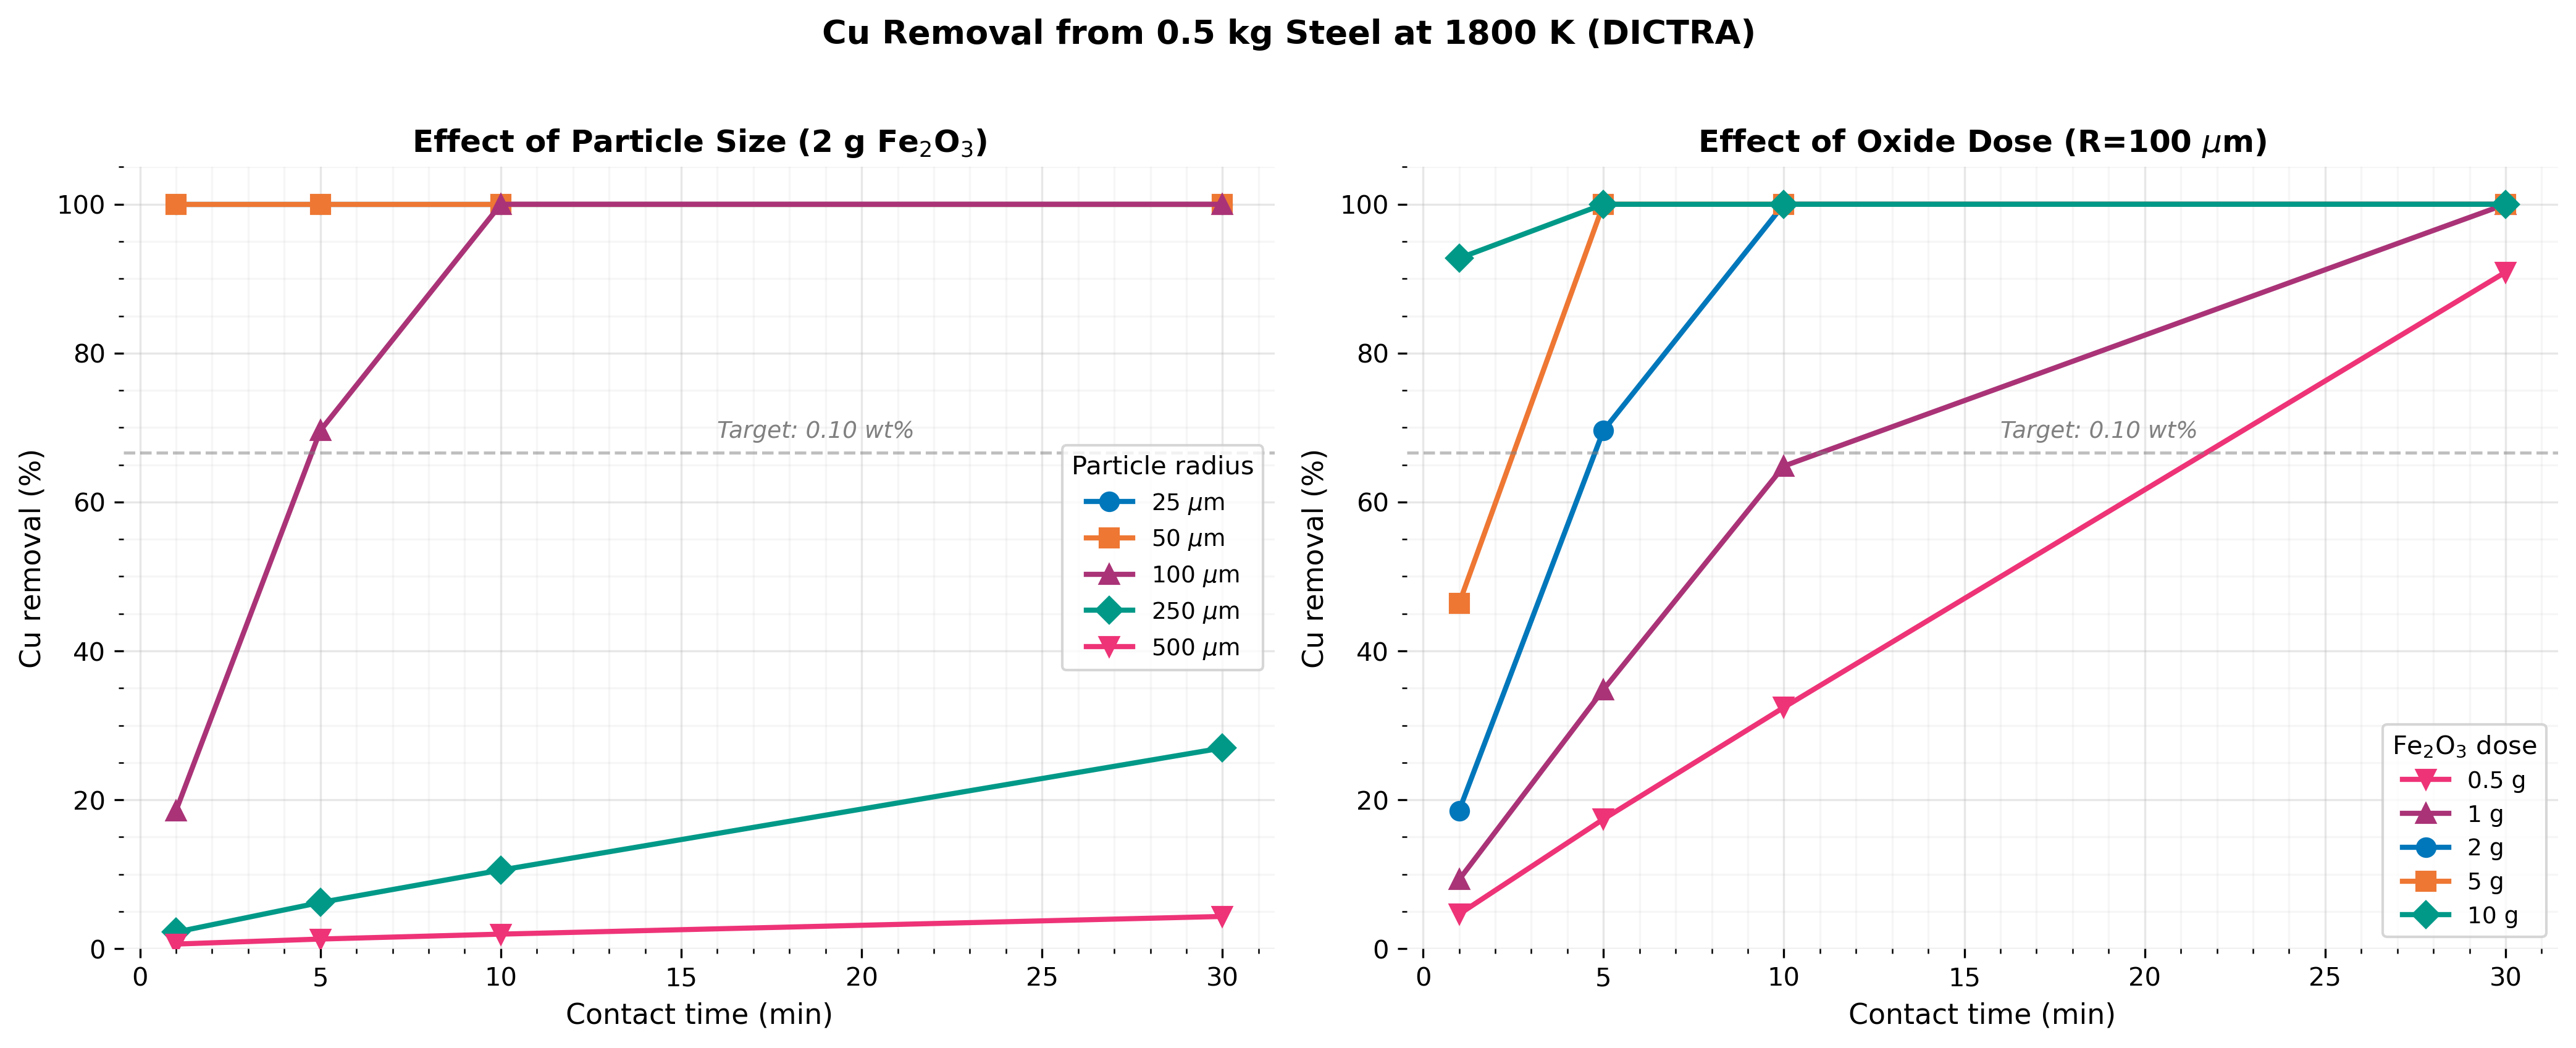
\includegraphics[width=\textwidth]{cu_removal_system_scale.png}
    \caption{System-scale Cu removal from \SI{0.5}{\kilogram} steel at \SI{1800}{\kelvin}. Left: effect of particle size at fixed 2\,g Fe$_2$O$_3$ dose. Right: effect of oxide dose at fixed $R = \SI{100}{\micro\meter}$. Dashed line marks the 0.10\,wt\% Cu target (67\% removal). Generated by \texttt{plot\_cu\_removal\_rate.py}.}
    \label{fig:cu_removal_system}
\end{figure}

\begin{insight}[Activity BC vs.\ Fixed Composition BC]
The original script used an activity boundary condition ($a_{\text{Cu}} = 0.001$) at the particle surface. This caused DICTRA to drive Cu \textit{toward} the surface (100\,wt\% Cu) instead of away from it. Root cause: the Fe-Cu liquid miscibility gap creates two compositions with the same activity. DICTRA picked the Cu-rich root ($\sim$100\% Cu) instead of the Fe-rich root ($\sim$0.01\% Cu). Switching to a fixed composition BC (Cu = 0.01\,wt\%) eliminated the ambiguity. Lesson: use activity BCs only when the activity-composition mapping is monotonic.
\end{insight}

\subsection{Experiment Plan}

Fontana Lab induction furnace with graphite crucible inside Al$_2$O$_3$ containment. Key variables:
\begin{itemize}[leftmargin=*]
    \item Steel: recycled scrap from Honda (XRF-characterized) or CDME
    \item Slag: 1--2 candidate oxides, possibly with Na$_2$S or CaF$_2$ flux
    \item Oxide dose: 1--2\,wt\% (from mass balance, Table~\ref{tab:mass_balance})
    \item Temperature: \SI{1500}{\celsius}--\SI{1600}{\celsius}
    \item Analysis: XRF (OES is currently down)
    \item Timeline: oxide ordering by April, experiments May--June
\end{itemize}


%%%%%%%%%%%%%%%%%%%%%%%%%%%%%%%%%%%%%%%%%%%%%%%%%%%%%%%%%%%%%%%%%%%%%%%%%%%%%%%
% 13. TECHNICAL PITFALLS AND LESSONS
%%%%%%%%%%%%%%%%%%%%%%%%%%%%%%%%%%%%%%%%%%%%%%%%%%%%%%%%%%%%%%%%%%%%%%%%%%%%%%%
\section{Technical Pitfalls and Lessons Learned}

\begin{enumerate}[leftmargin=*]
    \item \textbf{GM is per mole of atoms, not formula units.} Multiply by atoms/formula. Getting this wrong gives energies off by 5--7$\times$.

    \item \textbf{O$_2$ reference = $2 \times$ GM(pure O).} TC-Python treats O as atomic, not molecular.

    \item \textbf{Set $N-1$ mole fractions.} The last element fills the remainder. Setting all $N$ overconstrains the system.

    \item \textbf{Empty element list = file existence check only.} Does not verify the database can load or has the needed elements/phases.

    \item \textbf{Kinetic System API $\neq$ thermodynamic System API.} The object from the kinetic database selector has different methods (\texttt{get\_phases\_in\_system()} not \texttt{get\_phase\_names()}).

    \item \textbf{Citrix clipboard corrupts binary files.} Always transfer via ZIP download from GitHub, never copy-paste.

    \item \textbf{``Top $N$ by pure $\Delta G$'' is a bad filter for dilute systems.} Multi-Cu products rank high by pure $\Delta G$ but get crushed by the activity penalty. Must select candidates under actual conditions.

    \item \textbf{SSUB3 is unreliable for complex oxides.} B$_2$O$_3$ from SSUB3 was 145\% off literature values. Only use SSUB3 as a last resort, with verification.

    \item \textbf{Flat $a_{\text{Cu}}$ is not a bug, it's the Gibbs Phase Rule.} In a 2-phase field at fixed $T, P$, activity is invariant along the tie line. Sweeping overall composition changes phase amounts, not phase compositions.

    \item \textbf{Dr.\ Zhang's FeO skepticism was about the binary reaction.} He was correct that Cu cannot reduce FeO. The ternary spinel reaction (Cu $+$ 2FeO $+$ O$_2 \to$ CuFe$_2$O$_4$) is a different mechanism that he himself asked us to check.
\end{enumerate}


%%%%%%%%%%%%%%%%%%%%%%%%%%%%%%%%%%%%%%%%%%%%%%%%%%%%%%%%%%%%%%%%%%%%%%%%%%%%%%%
% 14. GLOSSARY
%%%%%%%%%%%%%%%%%%%%%%%%%%%%%%%%%%%%%%%%%%%%%%%%%%%%%%%%%%%%%%%%%%%%%%%%%%%%%%%
\section{Glossary}

\begin{description}[leftmargin=!, labelwidth=2.2cm]
    \item[CALPHAD] Calculation of Phase Diagrams --- computational thermodynamics method
    \item[DICTRA] Diffusion Controlled Transformations --- 1D multicomponent diffusion solver
    \item[TCOX14] Thermo-Calc oxide thermodynamic database (version 14)
    \item[TCFE13] Thermo-Calc steel thermodynamic database (version 13)
    \item[MOBFE8] Thermo-Calc steel mobility database (version 8)
    \item[GM] Gibbs energy per mole of atoms (TC-Python output)
    \item[IONIC\_LIQ] Two-sublattice ionic liquid model for oxide melts
    \item[$a_{\text{Cu}}$] Activity of Cu --- effective thermodynamic concentration
    \item[$\gamma_{\text{Cu}}$] Raoultian activity coefficient of Cu in liquid Fe
    \item[Hot shortness] Surface cracking during hot working caused by Cu grain boundary segregation
    \item[Basicity] Ratio of basic to acidic oxides in slag; controls activity coefficients
    \item[OLI] Software for aqueous electrolyte thermodynamics (uses MSE model)
    \item[MQM] Modified Quasichemical Model (FactSage's slag modeling approach)
    \item[SER] Stable Element Reference (enthalpy reference state in CALPHAD)
\end{description}


%%%%%%%%%%%%%%%%%%%%%%%%%%%%%%%%%%%%%%%%%%%%%%%%%%%%%%%%%%%%%%%%%%%%%%%%%%%%%%%
% APPENDIX A: CHRONOLOGICAL LAB ENTRIES
%%%%%%%%%%%%%%%%%%%%%%%%%%%%%%%%%%%%%%%%%%%%%%%%%%%%%%%%%%%%%%%%%%%%%%%%%%%%%%%
\newpage
\appendix
\section{Chronological Lab Entries}
\label{sec:lab_entries}

This section records work in chronological order, showing how the project evolved from initial scoping through thermodynamic screening to kinetics exploration.

\subsection{January 23--26, 2026: Project Kickoff}

\textbf{Jan 23}: Project selected (Honda CALPHAD Cu removal). Initial folder structure created.

\textbf{Jan 26}: Kickoff meeting with Prof.\ Luo and Dr.\ Zhang via Zoom (10:28--10:54 AM). Established project scope: use CALPHAD to screen oxide materials for Cu removal from recycled steel. HW1 Meeting Report written and formatted with OSU-branded LaTeX template.

\subsection{January 31 -- February 4, 2026: First Calculations}

\textbf{Jan 31}: Created pyCALPHAD simulation folder. Built Ellingham diagram analysis (\texttt{cu\_ceramic\_affinity.py}) using literature data. Key finding: Cu oxides are least stable, so direct oxide reduction will not work. Created GitHub repo: \texttt{dimascad/honda-calphad}.

\textbf{Feb 1}: Built interactive Marimo notebook (\texttt{cu\_ceramic\_thermodynamics.py}) with temperature slider and oxide selector. Deployed to Molab. Created \texttt{DOCUMENTATION.tex} and \texttt{THERMOCALC\_GUIDE.tex}.

\textbf{Feb 4}: \textbf{First VM run.} Ran \texttt{extract\_oxide\_gibbs.py} on OSU ETS VM using Thermo-Calc TCOX14 database. Fixed three critical bugs:
\begin{enumerate}[leftmargin=*]
    \item GM normalization: per-atom $\to$ per-formula (off by 5--7$\times$)
    \item O$_2$ reference: $G_{\text{O}_2} = 2 \times \texttt{GM}$ (was using $1\times$)
    \item Two-phase mixture: was reading mixture energy instead of single-phase
\end{enumerate}
Successfully extracted $\Delta G_f$ for 7 oxides $\times$ 31 temperatures. Created Ellingham diagram with real TCOX14 data.

\subsection{February 12, 2026: Dr.\ Zhang Meeting: Direction Shift}

\textbf{Advisor meeting} (2:00--2:40 PM, 2165 Fontana Lab) with Dr.\ Zhang:

\begin{quote}
``We want to use the oxide to capture the copper. Last time, [Al$_2$O$_3$] worked because of the spinel reaction.''
\end{quote}

Key outcomes:
\begin{itemize}[leftmargin=*]
    \item Dr.\ Zhang \textbf{confirmed} Ellingham results are correct: Cu$_2$O is least stable
    \item Al$_2$O$_3$ tested experimentally last year: some Cu reduction but Na$_2$S salt was better (95\%, per Zhang)
    \item \textbf{New direction}: Model ternary compound formation (Cu + MO$_x$ + O$_2 \to$ CuMO$_y$), not binary exchange
    \item Screening table required: oxide name, density, toxicity, reaction $\Delta G$, cost
    \item Timeline: 2 weeks for calculations $\to$ meet end of March $\to$ Honda call after
\end{itemize}

Also submitted HW2 Project Charter (Feb 11).

\subsection{March 12, 2026: Screening Pipeline Complete}

\textbf{Full-day session.} Expanded from 7 to 18 oxides. Completed the screening table with all 10 candidate oxides having computed $\Delta G_{\text{rxn}}$ values, then ran the 18-oxide TCOX14 extraction on the VM (15 direct, 2 from SSUB3 fallback for PbO and CeO$_2$, plus partial B$_2$O$_3$). Built \texttt{Oxide\_Screening\_Complete.xlsx} with 5 sheets and cell formulas tracing the full GM $\to$ kJ/mol\,O$_2$ normalization pipeline.

Swept the entire periodic table: 47 oxides evaluated, 7 ``moonshots'' selected (NiO, CoO, PbO, B$_2$O$_3$, V$_2$O$_5$, La$_2$O$_3$, CeO$_2$). PbO turned out to be an interesting edge case: $\Delta G_{\text{rxn}} = -34.7$ kJ at \SI{727}{\celsius} (Cu CAN reduce it at low $T$) but $+136.2$ kJ at \SI{1527}{\celsius}. SSUB3 reliability was mixed: B$_2$O$_3$ was 145\% off literature values (rejected), CeO$_2$ was 19\% off (accepted with caveat).

\subsection{March 13, 2026: Ternary Breakthrough}

\textbf{Dr.\ Zhang meeting (11 AM):} presented 18-oxide screening. Dr.\ Zhang said ``good work'' and directed the ternary modeling effort.

\textbf{Morning:} Created \texttt{extract\_ternary\_reactions.py} and \texttt{compute\_ternary\_dG.py}. Pushed to GitHub.

\textbf{Evening, VM extraction:} Ran ternary extraction on OSU VM. \textbf{ALL 16 REACTIONS FAVORABLE.} Every Cu + MO$_x$ + O$_2 \to$ CuMO$_y$ reaction has $\Delta G < 0$ at \SI{1800}{\kelvin}. Top 3: CuFe$_2$O$_4$ ($-112$ kJ), Cu$_3$V$_2$O$_8$ ($-109$ kJ), CuMn$_2$O$_4$ ($-64$ kJ).

\textbf{Late evening, validation suite:} Ran all 5 VM scripts (CuFe$_2$O$_4$ decomposition, Cu activity, $\Delta G$ vs.\ $T$, slag basicity, phase maps) and all 6 local post-processing scripts. Verification: 136 overlapping $\Delta G$ points matched to 0.00 kJ.

Key discoveries:
\begin{itemize}[leftmargin=*]
    \item No crystalline ternary phase survives at \SI{1800}{\kelvin}; Cu capture = slag dissolution
    \item CuFe$_2$O$_4$: 41\% Cu-capture, 59\% Fe-oxidation. Cu-capture alone is favorable.
    \item Cu activity is flat in 2-phase fields (Gibbs Phase Rule, not a code bug)
    \item V$_2$O$_5$ has \textbf{two} products: Cu$_3$V$_2$O$_8$ (unfavorable dilute) and CuV$_2$O$_6$ (marginal)
\end{itemize}

\subsection{March 14, 2026: DICTRA Kinetics Testing}

Pivoted from thermodynamics (``does it react?'') to kinetics (``how fast?'').

\textbf{DICTRA test script} (\texttt{test\_dictra\_diffusion.py}): 6-phase script probing the TC-Python diffusion API on the OSU VM:
\begin{enumerate}[leftmargin=*]
    \item Database compatibility matrix: 312 combinations (4 thermo $\times$ 13 mobility $\times$ 6 element sets)
    \item System API exploration: discovered \texttt{get\_phases\_in\_system()} (not \texttt{get\_phase\_names()})
    \item Single-region diffusion: Cu gradient in FCC austenite
    \item $D_{\text{Cu}}$ vs.\ $T$: diffusion coefficients at 8 temperatures
    \item Two-region interface: steel $|$ slag boundary
    \item Boundary conditions: activity-based, cylindrical, spherical geometry
\end{enumerate}

Results ($\sim$1 hour runtime, 150 KB log):
\begin{itemize}[leftmargin=*]
    \item \textbf{Phase 1--2 SUCCEEDED:} 232/312 combos loaded; 40 unique thermo+mobility pairs support diffusion. Correct API method discovered: \texttt{get\_phases\_in\_system()}.
    \item \textbf{Phase 3--6 FAILED:} Script bugs (wrong phase enumeration methods, empty phases list, undefined variable). All three fixed.
    \item MOBFE9, MOBOX1/2: not found on VM. MOBFE8/7/6/5 all work.
    \item \texttt{PhaseComposition} class not in \texttt{tc\_python} namespace.
    \item Log archived: \texttt{data/tcpython/logs/2026-03-14\_dictra\_capability\_test.rtf}
\end{itemize}

Script fixed and ready for re-run. Added LIQUID phase support at \SI{1800}{\kelvin}.

\textbf{Run 3 results} (6:42 PM, 30 min runtime):
\begin{itemize}[leftmargin=*]
    \item \textbf{Phase 3 confirmed:} Cu diffusion in FCC\_A1 at 1200\,K, 50-point profile.
    \item \textbf{Phase 4:} $D_{\text{Cu}} = 9.63 \times 10^{-10}$\,m$^2$/s in LIQUID at 1773--1873\,K. Independently confirms Hino \& Ito (2010) literature value ($\sim 10^{-9}$). Solid-state values below grid resolution at 1\,s sim time.
    \item \textbf{Phase 5 Test B:} Steel/slag interface (FCC\_A1 $|$ IONIC\_LIQ\#2) at 1800\,K ran successfully. Cu partitions across the boundary. Test A failed due to incomplete composition profile (script bug, not API).
    \item \textbf{Phase 6:} All 4 tests passed: fixed-composition BC, activity BC ($a_{\text{Cu}} = 0.001$), cylindrical (50\,$\mu$m radius), spherical (center depleted to 0.04\,wt\% from 0.30\,wt\% surface).
    \item Log archived: \texttt{data/tcpython/logs/2026-03-14\_dictra\_run3\_642pm.rtf}
\end{itemize}

\begin{insight}[DICTRA Validates Literature and Enables Kinetic Modeling]
The computed $D_{\text{Cu}} = 9.63 \times 10^{-10}$\,m$^2$/s at 1800\,K matches the Hino \& Ito (2010) reference value of $\sim 10^{-9}$\,m$^2$/s for impurity diffusion in liquid iron. With steel/slag interface modeling, activity-based BCs, and spherical geometry all confirmed working, the DICTRA API can now model Cu transport from liquid steel into oxide particles: the core kinetic question for the Honda project.
\end{insight}

\subsection{March 14, 2026: Unified Workbook}

Compiled all screening and validation data into \texttt{Cu\_Removal\_Unified.xlsx} (15 tabs). Analysis tabs use Excel cell formulas that reference the raw data tabs, so every number is traceable: click any cell to see where it came from. Tabs are color-coded: blue for analysis, green for derived results, gray for raw TC-Python output.

\textbf{Excel charts added} (live, update with data changes):
\begin{itemize}[leftmargin=*]
    \item CuFe$_2$O$_4$ DeepDive: 3-series line chart (total $\Delta G$, alternative, Fe-oxidation contribution)
    \item Activity\_and\_Slag: 7-product sensitivity chart ($\Delta G_{\text{eff}}$ vs.\ $\gamma_{\text{Cu}}$), colors matched to matplotlib figures
    \item Normalization: horizontal bar chart showing $\Delta G^\circ$ per mol O$_2$ at \SI{1800}{\kelvin} for all 17 binary oxides
\end{itemize}

\textbf{Data provenance table} on Dashboard enhanced with ``Generating Script'' column containing clickable GitHub hyperlinks to each script's source code.

\begin{insight}[Activity Coefficient Verification]
$\gamma_{\text{Cu}} = 8.5$ confirmed from Hino \& Ito (2010), \textit{Thermodynamic Data for Steelmaking}, Tohoku University Press. Alternative: Sigworth \& Elliott (1974, \textit{Metal Science}, 755+ citations) give $\sim$10. Literature range 5--13. Both citations verified via web search.
\end{insight}


\subsection{March 14, 2026: Experiment Design Tools}

Built two tools connecting thermodynamic screening to experiment design:

\textbf{Mass balance calculator} (\texttt{screening/mass\_balance\_calculator.py}): computes stoichiometric oxide requirements for all 5 top candidates. For \SI{0.5}{\kilogram} steel going 0.30\% $\to$ 0.10\% Cu, Fe$_2$O$_3$ needs only \SI{7.5}{\gram} at 3$\times$ excess (1.5\,wt\%). V$_2$O$_5$ is most efficient at \SI{2.9}{\gram} (0.57\,wt\%) because each mol captures 3 Cu. Particle size sweep shows $R = 50$--\SI{100}{\micro\meter} is optimal: diffusion time $r^2/2D \approx 1$--5\,s (liquid-phase transport is essentially instantaneous vs.\ experiment hold times of 10--30\,min).

\textbf{Cu removal rate script} (\texttt{simulations/tcpython/cu\_removal\_rate.py}): DICTRA spherical particle model. A \SI{5}{\milli\meter} steel shell surrounds the particle with Cu = 0.01\,wt\% at the surface (fixed composition BC) and closed far-field BC. Sweeps 5 radii $\times$ 4 contact times = 20 calculations. Successfully executed on VM (see lab entry below).

\textbf{Accuracy audit} of all project numbers: 25 claims checked across thermodynamic values, literature references, and internal consistency. Zero substantive errors found. Fixed one broken URL in \texttt{capstone.bib} (911Metallurgist page had moved).

\textbf{CLAUDE.md pruned:} 472 $\to$ 323 lines. Session log history (Jan 23 -- Mar 12) archived to \texttt{SESSION\_LOG.md}. Stale action items removed.


\subsection{March 14, 2026: DICTRA Cu Removal Rate --- 20/20 Success}

Ran \texttt{cu\_removal\_rate.py} on the OSU VM. Four iterations to get it right:

\textbf{Run 1:} \texttt{TCPython()} returns a wrapper, not the session. Fixed by using \texttt{TCPython().\_\_enter\_\_()} to get the actual API object.

\textbf{Run 2:} Script selected FCC\_A1 as diffusion phase at \SI{1800}{\kelvin}. Steel is liquid above $\sim$\SI{1723}{\kelvin}. Phase selection logic had a bug: after finding LIQUID, a fallback check \texttt{if diff\_phase == "LIQUID"} was always true, overwriting with FCC\_A1. Fixed by using \texttt{None} as sentinel.

\textbf{Run 3:} Activity BC ($a_{\text{Cu}} = 0.001$) drove Cu to 100\,wt\% at the particle surface instead of depleting it. All 20 calculations returned negative \texttt{cu\_captured\_mg}. Root cause: Fe-Cu liquid miscibility gap. At \SI{1800}{\kelvin}, two liquid compositions satisfy any given $a_{\text{Cu}}$: one Fe-rich ($\sim$0.01\% Cu) and one Cu-rich ($\sim$100\% Cu). DICTRA picked the wrong root.

\textbf{Run 4 (success):} Replaced activity BC with fixed composition BC (Cu = 0.01\,wt\% at surface). All 20/20 calculations completed in 35 seconds. Cu at surface = 0.01\,wt\% (depleted from 0.30\%), positive capture values, depletion zones extending 250--\SI{500}{\micro\meter} into the steel. Output CSVs: \texttt{cu\_removal\_rate\_profiles.csv} (1200 rows) and \texttt{cu\_removal\_rate\_summary.csv} (20 rows).

\textbf{Figures generated:} Cu depletion profiles (Fig.~\ref{fig:cu_removal_profiles}), system-scale removal predictions (Fig.~\ref{fig:cu_removal_system}), and Cu captured per particle vs.\ time.

\textbf{File organization:} 9 loose RTF terminal logs archived from capstone root into \texttt{data/tcpython/logs/} with consistent \texttt{YYYY-MM-DD\_description.rtf} naming.

\begin{insight}[Miscibility Gap Traps in Boundary Conditions]
The Fe-Cu binary has a well-known liquid miscibility gap. Activity is not monotonic across it: the same $a_{\text{Cu}}$ maps to two compositions. DICTRA's root-finder has no way to know which one you want. Fixed composition BCs are always unambiguous. This is a general lesson: use activity BCs only when the activity-composition curve is monotonic in the phase of interest.
\end{insight}


%%%%%%%%%%%%%%%%%%%%%%%%%%%%%%%%%%%%%%%%%%%%%%%%%%%%%%%%%%%%%%%%%%%%%%%%%%%%%%%
% APPENDIX B: SCRIPT INDEX
%%%%%%%%%%%%%%%%%%%%%%%%%%%%%%%%%%%%%%%%%%%%%%%%%%%%%%%%%%%%%%%%%%%%%%%%%%%%%%%
\newpage
\section{Script Index}
\label{sec:script_index}

All scripts in the \texttt{honda-calphad} repository, organized by location and purpose.

\subsection{VM Scripts (\texttt{simulations/tcpython/})}

These run on the OSU ETS virtual machine where Thermo-Calc and TC-Python are installed.

\begin{table}[H]
\caption{TC-Python Scripts for OSU VM Execution}
\label{tab:vm_scripts}
\centering
\renewcommand{\arraystretch}{1.15}
\footnotesize
\begin{tabular}{|p{2.6in}|p{3.4in}|}
\hline
\rowcolor{headercolor}
\textcolor{white}{\textbf{Script}} & \textcolor{white}{\textbf{Purpose}} \\
\hline
\texttt{extract\_oxide\_gibbs.py} & Extract $\Delta G_f$ for 18 oxides from TCOX14 (Ellingham data). 500--2000K, 50K steps. \\
\hline
\rowcolor{altrow}
\texttt{extract\_ssub3\_fallback.py} & SSUB3 fallback for PbO, CeO$_2$, B$_2$O$_3$ (not in TCOX14). \\
\hline
\texttt{extract\_ternary\_reactions.py} & Ternary reaction GM extraction: Cu + MO$_x$ + O$_2 \to$ CuMO$_y$. 15 systems, 18 products. \\
\hline
\rowcolor{altrow}
\texttt{cufe2o4\_alternative\_reaction.py} & Decompose CuFe$_2$O$_4$ $\Delta G$ into Cu-capture vs.\ Fe-oxidation components. \\
\hline
\texttt{cu\_activity\_vs\_oxide.py} & Sweep $a_{\text{Cu}}$ vs.\ composition at \SI{1800}{\kelvin} for 4 ternary systems. \\
\hline
\rowcolor{altrow}
\texttt{dG\_vs\_T\_top6.py} & Fine $\Delta G$ vs.\ $T$ curves (25K steps) for top 6 candidates with phase tracking. \\
\hline
\texttt{slag\_composition\_effects.py} & Quaternary slag basicity effects on $a_{\text{Cu}}$ (Cu-Mn-Si-O, Cu-Al-Si-O). \\
\hline
\rowcolor{altrow}
\texttt{ternary\_phase\_map\_1800K.py} & 20$\times$20 composition grid phase mapping at \SI{1800}{\kelvin}. \\
\hline
\texttt{test\_dictra\_diffusion.py} & DICTRA capability test: database matrix, diffusion API, boundary conditions. \\
\hline
\rowcolor{altrow}
\texttt{check\_databases.py} & Probe which TC databases are installed on the VM. \\
\hline
\texttt{check\_mobox\_tcox.py} & Test MOBOX/TCOX mobility database availability. \\
\hline
\rowcolor{altrow}
\texttt{check\_vm\_capabilities.py} & General VM environment probe (Python version, packages). \\
\hline
\texttt{verify\_oxide\_data.py} & Cross-check extracted oxide data against literature values. \\
\hline
\rowcolor{altrow}
\texttt{test\_tcox\_api.py} & Early API exploration script for TCOX14 capabilities. \\
\hline
\texttt{cu\_al\_o\_phase\_stability.py} & Cu-Al-O phase stability exploration. \\
\hline
\rowcolor{altrow}
\texttt{cu\_activity\_combined\_db.py} & Attempt Cu activity with combined TCFE+TCOX database. \\
\hline
\rowcolor{altrow}
\texttt{cu\_removal\_rate.py} & DICTRA spherical particle model: Cu depletion around oxide particle in liquid steel. 5 radii $\times$ 4 times. \\
\hline
\end{tabular}
\end{table}

\subsection{Local Post-Processing Scripts (\texttt{screening/})}

These run locally on the Mac after copying CSVs from the VM.

\begin{table}[H]
\caption{Local Post-Processing and Analysis Scripts}
\label{tab:local_scripts}
\centering
\renewcommand{\arraystretch}{1.15}
\footnotesize
\begin{tabular}{|p{2.8in}|p{3.2in}|}
\hline
\rowcolor{headercolor}
\textcolor{white}{\textbf{Script}} & \textcolor{white}{\textbf{Purpose}} \\
\hline
\texttt{compute\_ternary\_dG.py} & Compute $\Delta G$ for all ternary reactions from raw GM data. \\
\hline
\rowcolor{altrow}
\texttt{compute\_reaction\_dG.py} & Compute binary reaction $\Delta G$ (Ellingham analysis). \\
\hline
\texttt{compute\_activity\_corrected\_dG.py} & Apply dilute Cu activity correction ($\gamma_{\text{Cu}} \cdot x_{\text{Cu}}$). \\
\hline
\rowcolor{altrow}
\texttt{analyze\_cufe2o4\_decomposition.py} & Split CuFe$_2$O$_4$ driving force into Cu-capture vs.\ Fe-oxidation. \\
\hline
\texttt{plot\_cu\_activity.py} & Figure: $a_{\text{Cu}}$ vs.\ oxide fraction for 4 systems. \\
\hline
\rowcolor{altrow}
\texttt{plot\_dG\_vs\_T.py} & Figure: $\Delta G$ vs.\ $T$ for top 6 candidates + verification. \\
\hline
\texttt{plot\_ternary\_phase.py} & Figures: ternary composition diagrams colored by dominant phase. \\
\hline
\rowcolor{altrow}
\texttt{plot\_slag\_effects.py} & Figure: $a_{\text{Cu}}$ vs.\ slag basicity ratio. \\
\hline
\texttt{update\_screening\_table.py} & Update screening CSV with computed values. \\
\hline
\rowcolor{altrow}
\texttt{compute\_activity\_corrected\_dG.py} & Activity-corrected $\Delta G$ for dilute Cu ($X_{\text{Cu}}=0.003$, $\gamma_{\text{Cu}}=8.5$). \\
\hline
\rowcolor{altrow}
\texttt{mass\_balance\_calculator.py} & Stoichiometric oxide requirements, particle counts, surface area, diffusion time estimates. \\
\hline
\texttt{plot\_cu\_removal\_rate.py} & Figures: Cu depletion profiles, per-particle capture, and system-scale removal from DICTRA data. \\
\hline
\rowcolor{altrow}
\texttt{build\_unified\_xlsx.py} & Build \texttt{Cu\_Removal\_Unified.xlsx}: 16-tab workbook with formula-driven analysis tabs and raw data tabs. \\
\hline
\end{tabular}
\end{table}

\subsection{Marimo Notebooks (\texttt{simulations/notebooks/})}

Interactive Python notebooks deployed to Molab for visualization.

\begin{table}[H]
\caption{Marimo Interactive Notebooks}
\label{tab:notebooks}
\centering
\renewcommand{\arraystretch}{1.15}
\footnotesize
\begin{tabular}{|p{2.5in}|p{3.5in}|}
\hline
\rowcolor{headercolor}
\textcolor{white}{\textbf{Script}} & \textcolor{white}{\textbf{Purpose}} \\
\hline
\texttt{ellingham\_diagram.py} & Interactive Ellingham diagram with oxide selector. Deployed at Molab. \\
\hline
\rowcolor{altrow}
\texttt{cu\_ceramic\_affinity.py} & Oxide stability comparison using literature data. \\
\hline
\texttt{cu\_o\_visualization.py} & Cu-O system visualization. \\
\hline
\rowcolor{altrow}
\texttt{cu\_o\_pycalphad.py} & pyCALPHAD-based Cu-O computation. \\
\hline
\texttt{compute\_cu\_o\_data.py} & Data generation for Cu-O plots. \\
\hline
\rowcolor{altrow}
\texttt{pycalphad\_cu\_fe\_example.py} & pyCALPHAD demonstration with Cu-Fe binary system. \\
\hline
\end{tabular}
\end{table}


%%%%%%%%%%%%%%%%%%%%%%%%%%%%%%%%%%%%%%%%%%%%%%%%%%%%%%%%%%%%%%%%%%%%%%%%%%%%%%%
% APPENDIX C: DATA FILES
%%%%%%%%%%%%%%%%%%%%%%%%%%%%%%%%%%%%%%%%%%%%%%%%%%%%%%%%%%%%%%%%%%%%%%%%%%%%%%%
\newpage
\section{Data Files}
\label{sec:data_files}

All raw data is stored in \texttt{data/tcpython/raw/}. Each CSV is produced by one VM script and consumed by one or more local post-processing scripts.

\begin{table}[H]
\caption{Raw Data Files from TC-Python VM Runs}
\label{tab:data_files}
\centering
\renewcommand{\arraystretch}{1.15}
\footnotesize
\begin{tabular}{|p{2.8in}|c|p{2.2in}|}
\hline
\rowcolor{headercolor}
\textcolor{white}{\textbf{File}} & \textcolor{white}{\textbf{Size}} & \textcolor{white}{\textbf{Source Script}} \\
\hline
\texttt{oxide\_gibbs\_energies.csv} & 54 kB & \texttt{extract\_oxide\_gibbs.py} \\
\hline
\rowcolor{altrow}
\texttt{ternary\_reaction\_energies.csv} & 92 kB & \texttt{extract\_ternary\_reactions.py} \\
\hline
\texttt{dG\_vs\_T\_top6.csv} & 57 kB & \texttt{dG\_vs\_T\_top6.py} \\
\hline
\rowcolor{altrow}
\texttt{cufe2o4\_alternative\_reaction.csv} & 5 kB & \texttt{cufe2o4\_alternative\_reaction.py} \\
\hline
\texttt{cu\_activity\_vs\_oxide.csv} & 7 kB & \texttt{cu\_activity\_vs\_oxide.py} \\
\hline
\rowcolor{altrow}
\texttt{slag\_composition\_effects.csv} & 4 kB & \texttt{slag\_composition\_effects.py} \\
\hline
\texttt{ternary\_phase\_map\_1800K.csv} & 106 kB & \texttt{ternary\_phase\_map\_1800K.py} \\
\hline
\rowcolor{altrow}
\texttt{cu\_removal\_rate\_summary.csv} & 2 kB & \texttt{cu\_removal\_rate.py} \\
\hline
\texttt{cu\_removal\_rate\_profiles.csv} & 85 kB & \texttt{cu\_removal\_rate.py} \\
\hline
\end{tabular}
\end{table}

All figures are stored in \texttt{figures/} as both PNG (for this document) and PDF (for vector-quality printing). Every figure has a corresponding script in the ``Source Script'' column of Table~\ref{tab:local_scripts}.


%%%%%%%%%%%%%%%%%%%%%%%%%%%%%%%%%%%%%%%%%%%%%%%%%%%%%%%%%%%%%%%%%%%%%%%%%%%%%%%
% APPENDIX D: SELECTED SCRIPTS
%%%%%%%%%%%%%%%%%%%%%%%%%%%%%%%%%%%%%%%%%%%%%%%%%%%%%%%%%%%%%%%%%%%%%%%%%%%%%%%
\newpage
\section{Selected Scripts}
\label{sec:scripts}

This appendix includes the scripts needed to reproduce the key results in this notebook. Only scripts that generate primary data or perform critical analysis are included; plotting scripts and Excel builders are omitted (they are in the GitHub repository). Scripts are printed in order of the analysis pipeline: data extraction first, then post-processing.

Each script has a brief introduction explaining what it does, what database it uses, where it runs, and which section of the notebook uses its output.

% Smaller font for code to keep page count reasonable
% literate handles Unicode chars that appear in our Python scripts
\lstset{
    basicstyle=\ttfamily\scriptsize,
    numbers=left,
    numberstyle=\tiny\color{darkgray},
    numbersep=5pt,
    extendedchars=true,
    literate={°}{{$^\circ$}}1 {→}{{$\rightarrow$}}1 {—}{{---}}1 {₂}{{$_2$}}1 {₃}{{$_3$}}1 {₄}{{$_4$}}1
}

% ---- Script 1 ----
\subsection{extract\_oxide\_gibbs.py}
\label{script:extract_oxide_gibbs}

\textbf{Runs on:} OSU ETS VM (requires TC-Python + TCOX14~\cite{TCOX14})\\
\textbf{Runtime:} $\sim$5 minutes\\
\textbf{Output:} \texttt{data/tcpython/raw/oxide\_gibbs\_energies.csv}\\
\textbf{Used in:} Section~\ref{fig:ellingham} (Ellingham diagram), Normalization tab of unified workbook

Extracts Gibbs energy of formation ($\Delta G_f$) for 18 binary oxides from TCOX14 over 500--2000\,K in 50\,K steps. For each oxide, it computes: (1) $G$ of the oxide phase at its stoichiometric composition, (2) $G$ of the pure metal reference, and (3) $G$ of O$_2$ gas. The formation energy is $\Delta G_f = G_{\text{oxide}} - n\,G_{\text{metal}} - m\,G_{\text{O}_2}$, normalized per mole O$_2$ for the Ellingham diagram. This is the foundation of the entire screening pipeline.

\lstinputlisting[language=Python]{../simulations/tcpython/extract_oxide_gibbs.py}

% ---- Script 2 ----
\cleardoublepage
\subsection{extract\_ternary\_reactions.py}
\label{script:extract_ternary}

\textbf{Runs on:} OSU ETS VM (requires TC-Python + TCOX14~\cite{TCOX14})\\
\textbf{Runtime:} $\sim$10 minutes\\
\textbf{Output:} \texttt{data/tcpython/raw/ternary\_reaction\_energies.csv} (414 rows)\\
\textbf{Used in:} Section~4 (Ternary Reaction Modeling), Table~\ref{tab:ternary_ranking}

The most important script in the project. For each of 15 Cu-M-O ternary systems, it sets the composition to the known ternary compound stoichiometry (e.g., $x_{\text{Cu}}=1/7$, $x_{\text{Fe}}=2/7$, $x_{\text{O}}=4/7$ for CuFe$_2$O$_4$) and computes the system Gibbs energy via TC-Python equilibrium. The reaction $\Delta G$ is the difference between product and reactant system energies. A negative value means the oxide captures copper.

\lstinputlisting[language=Python]{../simulations/tcpython/extract_ternary_reactions.py}

% ---- Script 3 ----
\cleardoublepage
\subsection{cufe2o4\_alternative\_reaction.py}
\label{script:cufe2o4_alt}

\textbf{Runs on:} OSU ETS VM (requires TC-Python + TCOX14~\cite{TCOX14})\\
\textbf{Runtime:} $\sim$3 minutes\\
\textbf{Output:} \texttt{data/tcpython/raw/cufe2o4\_alternative\_reaction.csv}\\
\textbf{Used in:} Section~10 (CuFe$_2$O$_4$ Deep Dive)

CuFe$_2$O$_4$ has the strongest driving force ($-112$ kJ), but how much of that comes from Cu capture vs.\ Fe$^{2+} \to$ Fe$^{3+}$ oxidation? This script computes the alternative reaction using Fe$_2$O$_3$ (Fe already at $+3$) instead of FeO. The difference isolates the Fe-oxidation bonus. Result: Cu capture alone contributes $-46$ kJ (41\%), confirming the reaction is not just riding on iron oxidation.

\lstinputlisting[language=Python]{../simulations/tcpython/cufe2o4_alternative_reaction.py}

% ---- Script 4 ----
\cleardoublepage
\subsection{cu\_activity\_vs\_oxide.py}
\label{script:cu_activity}

\textbf{Runs on:} OSU ETS VM (requires TC-Python + TCOX14~\cite{TCOX14})\\
\textbf{Runtime:} $\sim$5 minutes\\
\textbf{Output:} \texttt{data/tcpython/raw/cu\_activity\_vs\_oxide.csv}\\
\textbf{Used in:} Section~7 (Cu Activity and the Gibbs Phase Rule), Fig.~\ref{fig:cu_activity}

Sweeps Cu mole fraction from 0.90 to 0.05 in four Cu-M-O systems at 1800\,K, recording $a_{\text{Cu}}$ via \texttt{AC(CU)}. The result was initially puzzling: activity is flat across the entire sweep. This turned out to be a textbook Gibbs Phase Rule consequence (Section~7), not a bug.

\lstinputlisting[language=Python]{../simulations/tcpython/cu_activity_vs_oxide.py}

% ---- Script 5 ----
\cleardoublepage
\subsection{slag\_composition\_effects.py}
\label{script:slag_effects}

\textbf{Runs on:} OSU ETS VM (requires TC-Python + TCOX14~\cite{TCOX14})\\
\textbf{Runtime:} $\sim$5 minutes\\
\textbf{Output:} \texttt{data/tcpython/raw/slag\_composition\_effects.csv}\\
\textbf{Used in:} Section~6.4 (Slag Basicity Results), Fig.~\ref{fig:slag_basicity}

Tests whether slag basicity affects Cu capture. Fixes $x_{\text{Cu}} = 0.003$ (steelmaking level) and varies the basic-to-acidic oxide ratio in two quaternary systems: Cu-Mn-Si-O and Cu-Al-Si-O. If $a_{\text{Cu}}$ decreases with increasing basicity, a more basic slag promotes Cu capture. Result: MnO:SiO$_2$ ratio is a tunable knob ($-17$\% $a_{\text{Cu}}$); Al$_2$O$_3$:SiO$_2$ has no effect.

\lstinputlisting[language=Python]{../simulations/tcpython/slag_composition_effects.py}

% ---- Script 6 ----
\cleardoublepage
\subsection{compute\_ternary\_dG.py}
\label{script:compute_ternary}

\textbf{Runs on:} Local (post-processing, no TC-Python needed)\\
\textbf{Runtime:} $<$1 second\\
\textbf{Input:} \texttt{data/tcpython/raw/ternary\_reaction\_energies.csv}\\
\textbf{Output:} \texttt{screening/ternary\_screening\_results.csv}\\
\textbf{Used in:} Section~4, Ternary\_Verdicts tab of unified workbook

Reads the raw ternary reaction energies from Script~2 and produces the ranked summary table: product name, parent oxide, $\Delta G$ at three key temperatures (727, 1227, 1527\,$^\circ$C), stable phases, and a FAVORABLE/UNFAVORABLE verdict. This is the script that confirmed all 16 reactions are favorable.

\lstinputlisting[language=Python]{../screening/compute_ternary_dG.py}

% ---- Script 7 ----
\cleardoublepage
\subsection{compute\_activity\_corrected\_dG.py}
\label{script:activity_corrected}

\textbf{Runs on:} Local (post-processing, no TC-Python needed)\\
\textbf{Runtime:} $\sim$2 seconds\\
\textbf{Input:} \texttt{data/tcpython/raw/ternary\_reaction\_energies.csv}\\
\textbf{Output:} \texttt{data/tcpython/processed/activity\_corrected\_dG.csv}, sensitivity figures\\
\textbf{Used in:} Section~\ref{sec:activity_correction} (Activity Correction), Figs.~\ref{fig:dG_corrected},~\ref{fig:gamma_sensitivity}

The script that reshuffled everything. Takes the pure-Cu $\Delta G$ values and applies the dilute-Cu activity penalty: $\Delta G_{\text{eff}} = \Delta G_{\text{pure}} + n_{\text{Cu}} \cdot RT\ln(a_{\text{Cu}})$. Uses $\gamma_{\text{Cu}} = 8.5$~\cite{Hino2010} and $x_{\text{Cu}} = 0.003$. Also runs a sensitivity sweep over $\gamma_{\text{Cu}} = 3$--15 to test sensitivity. This is where Cu$_3$V$_2$O$_8$ (ranked \#2 by pure $\Delta G$) gets eliminated and CuFe$_2$O$_4$ emerges as the clear winner.

\lstinputlisting[language=Python]{../screening/compute_activity_corrected_dG.py}


\vfill
\begin{center}
\textit{Last updated: \today}
\end{center}

%%%%%%%%%%%%%%%%%%%%%%%%%%%%%%%%%%%%%%%%%%%%%%%%%%%%%%%%%%%%%%%%%%%%%%%%%%%%%%%
% REFERENCES
%%%%%%%%%%%%%%%%%%%%%%%%%%%%%%%%%%%%%%%%%%%%%%%%%%%%%%%%%%%%%%%%%%%%%%%%%%%%%%%
\newpage
\begin{thebibliography}{99}

\bibitem{Daehn2019}
K.~E. Daehn, A.~Cabrera Serrenho, and J.~M. Allwood,
``Finding the most efficient way to remove residual copper from steel scrap,''
\textit{Metall.\ Mater.\ Trans.\ B}, vol.~50, pp.~1225--1240, 2019.
doi:~10.1007/s11663-019-01537-9

\bibitem{Lukas2007}
H.~L. Lukas, S.~G. Fries, and B.~Sundman,
\textit{Computational Thermodynamics: The Calphad Method}.
Cambridge University Press, 2007.

\bibitem{Andersson2002}
J.-O. Andersson, T.~Helander, L.~H\"{o}glund, P.~Shi, and B.~Sundman,
``Thermo-Calc \& DICTRA, computational tools for materials science,''
\textit{Calphad}, vol.~26, no.~2, pp.~273--312, 2002.
doi:~10.1016/S0364-5916(02)00037-8

\bibitem{TCOX14}
Thermo-Calc Software,
``TCS Metal Oxide Solutions Database (TCOX14),''
\url{https://thermocalc.com/products/databases/metal-oxide-solutions/}, accessed Mar.\ 2026.

\bibitem{SSUB3}
Thermo-Calc Software,
``SGTE Substances Database (SSUB3),''
\url{https://thermocalc.com/products/databases/}, accessed Mar.\ 2026.

\bibitem{Gaskell2024}
D.~R. Gaskell and D.~E. Laughlin,
\textit{Introduction to the Thermodynamics of Materials}, 7th~ed.
CRC Press, 2024.

\bibitem{Hillert2007}
M.~Hillert,
\textit{Phase Equilibria, Phase Diagrams and Phase Transformations: Their Thermodynamic Basis}, 2nd~ed.
Cambridge University Press, 2007.

\bibitem{Porter2021}
D.~A. Porter, K.~E. Easterling, and M.~Y. Sherif,
\textit{Phase Transformations in Metals and Alloys}, 4th~ed.
CRC Press, 2021.

\bibitem{Hino2010}
M.~Hino and K.~Ito, Eds.,
\textit{Thermodynamic Data for Steelmaking}.
Tohoku University Press, 2010.

\bibitem{Sigworth1974}
G.~K. Sigworth and J.~F. Elliott,
``The thermodynamics of liquid dilute iron alloys,''
\textit{Metal Science}, vol.~8, pp.~298--310, 1974.
doi:~10.1179/msc.1974.8.1.298

\bibitem{Seetharaman2005}
S.~Seetharaman, Ed.,
\textit{Fundamentals of Metallurgy}.
Woodhead Publishing, 2005.

\bibitem{911metallurgist}
911~Metallurgist,
``Removing copper from molten steel scrap,''
\url{https://www.911metallurgist.com/blog/removing-copper-molten-steel-scrap}, 2017.
Summarizes Bureau of Mines oxide injection experiments.

\bibitem{Brown2026CALPHAD}
J.~Brown,
``CALPHAD introduction,''
MSE 3321 Lecture, The Ohio State University, 2026.

\bibitem{Brown2026TC1}
J.~Brown and Y.~Ji,
``Equilibrium calculations (TC1),''
MSE 3321 Lab Handout, The Ohio State University, 2026.

\bibitem{Sundman1985}
B.~Sundman, B.~Jansson, and J.-O. Andersson,
``The Thermo-Calc databank system,''
\textit{Calphad}, vol.~9, no.~2, pp.~153--190, 1985.
doi:~10.1016/0364-5916(85)90021-5

\end{thebibliography}

\end{document}
